% Vorlage für eine Bachelorarbeit
% Siehe auch LaTeX-Kurs von Mathematik-Online
% www.mathematik-online.org/kurse
% Anpassungen für die Fakultät für Mathematik
% am KIT durch Klaus Spitzmüller und Roland Schnaubelt Dezember 2011

\documentclass[12pt,a4paper]{scrartcl}
% scrartcl ist eine abgeleitete Artikel-Klasse im Koma-Skript
% zur Kontrolle des Umbruchs Klassenoption draft verwenden


% die folgenden Packete erlauben den Gebrauch von Umlauten und ß
% in der Latex Datei
\usepackage[utf8]{inputenc}
% \usepackage[latin1]{inputenc} %  Alternativ unter Windows
\usepackage[T1]{fontenc}
\usepackage[ngerman]{babel}


\usepackage[pdftex]{graphicx}
\usepackage{latexsym}
\usepackage{amsmath,amssymb,amsthm}
\usepackage{setspace}
\usepackage{url}
\usepackage{mathtools}
\usepackage{enumitem}
\usepackage{float}
\usepackage{dsfont}
\usepackage{subfigure}
\usepackage[ruled,vlined,linesnumbered]{algorithm2e}
\usepackage{longtable}
\usepackage{tabularx}
\usepackage{pdfpages}


% Abstand obere Blattkante zur Kopfzeile ist 2.54cm - 15mm
\setlength{\topmargin}{-15mm}


% Umgebungen für Definitionen, Sätze, usw.
% Es werden Sätze, Definitionen etc innerhalb einer Section mit
% 1.1, 1.2 etc durchnummeriert, ebenso die Gleichungen mit (1.1), (1.2) ..
\theoremstyle{definition}
\newtheorem{Satz}{Satz}[section]
\newtheorem{Folgerung}[Satz]{Folgerung} 
\newtheorem{Definition}[Satz]{Definition} 
\newtheorem{Lemma}[Satz]{Lemma}	
\newtheorem{Beispiel}[Satz]{Beispiel}
\newtheorem{Annahme}[Satz]{Annahme}	   
\newtheorem{Bemerkung2}[Satz]{Bemerkung}
                  
\numberwithin{equation}{section} 

\newtheorem*{Bemerkung}{Bemerkung}

% einige Abkuerzungen
\newcommand{\C}{\mathbb{C}} % komplexe
\newcommand{\K}{\mathbb{K}} % komplexe
\newcommand{\R}{\mathbb{R}} % reelle
\newcommand{\Q}{\mathbb{Q}} % rationale
\newcommand{\Z}{\mathbb{Z}} % ganze
\newcommand{\N}{\mathbb{N}} % natuerliche

% eigene Definitionen
\newcommand{\dx}{\, \mathrm{d} x}
\newcommand{\da}{\, \mathrm{d} a}
\newcommand{\dt}{\, \mathrm{d} t}
\newcommand{\ds}{\, \mathrm{d} s}
\newcommand{\du}{\, \mathrm{d} u}
\newcommand{\dlam}{\, \mathrm{d} \lambda}
\newcommand{\dP}{\, \mathrm{d} \mathbb{P}}

\newcommand{\icol}[1]{%inline row vector
		\left(	\begin{smallmatrix}#1\end{smallmatrix} \right) %
	}
\newcommand{\abs}[1]{| #1 |}
\newcommand{\ubar}[1]{\underline{#1}{}}
\DeclareMathOperator{\dive}{div}
\DeclareMathOperator{\spann}{span}
\DeclareMathOperator{\conv}{conv}
\DeclareMathOperator{\supp}{supp}

\begin{document}
  % Keine Seitenzahlen im Vorspann
  \pagestyle{empty}
  
  
  % Titelblatt der Arbeit
  \begin{titlepage}

    
\includegraphics[scale=0.45]{kit-logo.jpg} 
    \vspace*{2cm} 

 \begin{center} \large 
    
    Bachelorarbeit
    \vspace*{2cm}

    {\huge Die Multilevel Monte Carlo Methode \vspace{2mm}\\ und deren Anwendung am Beispiel der \vspace{2mm} linearen\- Transportgleichung}
    \vspace*{2.5cm}

    Tim Buchholz
    \vspace*{1.5cm}

    20.04.20
    \vspace*{4.5cm}


    {Betreuung: Prof.Dr. Christian Wieners und M.Sc. Niklas Baumgarten \\[1cm]
    Fakultät für Mathematik \\
    Karlsruher Institut für Technologie}
  \end{center}
\end{titlepage}



  % Inhaltsverzeichnis
  \tableofcontents

\newpage
 


  % Ab sofort Seitenzahlen in der Kopfzeile anzeigen
  \pagestyle{headings}


% !TeX root = bachelorarbeit.tex

\section{Einleitung}

Monte Carlo Methoden sind weit verbreitet, um in unterschiedlichsten Situationen Erwartungswerte stochastischer Modelle zu schätzen.
So werden bei der Monte Carlo Quadratur, der wohl bekanntesten Anwendungen der Monte Carlo Methode, zufällig gleichverteilte Stützstellen dafür genutzt, den Erwartungswert der Funktionsauswertung an einer zufälligen Stützstelle zu bestimmen. Daraus lässt sich anschließend der approximierte Integralwert auf einer gegebenen Grundmenge bestimmen. 
Wir wollen Monte Carlo Methoden dazu nutzen, eine stochastische partielle Differentialgleichung zu lösen. 
Genauer betrachten wir eine stochastisch beeinflusste Zielgröße $ Q $ der Lösung der Differentialgleichung und fragen uns, welchen Wert $ \mathbb{E}[Q] $ nimmt $ Q $ im Mittel an? Wir suchen also nach einem Erwartungswert, was die Verwendung von Monte Carlo Methoden zumindest einmal nahelegt. 
Außerdem wollen wir uns dabei die Vorteile der sogenannten Multilevel Monte Carlo (MLMC) Methode zunutze machen. Diese wurde zunächst von Heinrich für Approximation von parameterabhängigen Integralen in hohen Dimensionen entwickelt (vgl. \cite{heinrich2001multilevel}) und anschließend unter anderem von  Giles auf stochastisch modellierte partielle Differentialgleichungen übertragen. Folgendes Zitat bringt die Vorteile auf den Punkt, welche die Multilevel Monte Carlo Methode in diesem Zusammenhang bietet:
\begin{quote}
	\textit{Monte Carlo methods are a very general and useful approach for the estimation of expectations arising from stochastic simulation. However, they can be computationally expensive, particularly when the cost of generating individual stochastic samples is very high, as in the case of stochastic PDEs. \\ Multilevel Monte Carlo is a recently developed approach which greatly reduces the computational cost by performing most simulations with low accuracy at a correspondingly low cost, with relatively few simulations being performed at high accuracy and a high cost.}  \\
	\rightline{Michael B. Giles in \cite{giles_2015}. \, \qquad \qquad }
\end{quote}
Das Lösen, bzw. in unserem Fall das Bestimmen eines Erwartungswert, von stochastisch modellierten partiellen Differentialgleichungen fallen in das Gebiet der Uncertainty Quantification. Dieses noch recht 'junge' Feld der Mathematik wird von Sullivan in \cite{sullivan2015introduction} als ein 'Zusammentreffen der Wahrscheinlichkeitstheorie, Numerik, Statistik und der echten Welt' beschrieben. \\
Die Thesis lässt sich aktuellen Arbeiten am Institut für Angewandte und Numerische Mathematik, wie etwa \cite{BAUMGARTEN2020}, zuordnen und soll daher zwar zum einen den theoretischen Hintergrund darlegen, aber auch einige Ergebnisse präsentieren, die im parallelen Finite Elemente System M++ \cite{siteM++} erzielt werden konnten, welches am Institut für Angewandte und Numerische Mathematik unter anderem von Herrn Prof. Dr. C. Wieners entwickelt wurde. \\
Konkret wollen wir vor allem die zeitabhängige lineare Transportgleichung betrachten. Dabei handelt es sich um ein weit verbreitetes Modellproblem, welches unter Anderem auch in \cite{di2011mathematical}, einem Standardwerk für Discontinuous Galerkin Methoden, zu finden ist. 
Dabei nutzen wir wie in \cite{di2011mathematical} die sogenannte 'method of lines': Zur numerischen Lösung der Differentialgleichung nutzen wir ein Discontinuous Galerkin Verfahren (DGV) im Ort und kombinieren diese zunächst semidiskrete Lösung mit einem geeigneten Zeitschrittverfahren. Aufgrund der Wahl eines Runge-Kutta Verfahrens erhalten wir somit ein Runge-Kutta Discontinuos Galerkin Verfahren. Einen Überblick über diese Verfahrensart findet man zum Beispiel auch in \cite{cockburn2001runge}.
Ebenfalls mit der Anwendung von Multilevel Monte Carlo Methoden auf eine Variante des Transportproblems mit Diffusion haben sich zum Beispiel auch Barth und Stein in \cite{barth2013multilevel} bzw. \cite{barth2019multilevel} oder Kumar et al. in \cite{kumar2018multigrid} beschäftigt. Mit Multilevel Monte Carlo Methoden im Allgemeinen haben sich neben den bereits erwähnten Giles und Barth auch Cliffe in \cite{cliffe2011multilevel}, Charrier in \cite{charrier2012strong} oder Teckentrup in \cite{teckentrup2013further}, um nur Einige zu nennen, befasst.
Um die eigentliche Idee der Multilevel Monte Carlo Methode in den Vordergrund zu rücken, wollen wir diese aber auch wie in \cite{heinrich2001multilevel} am Beispiel der numerischen Integration betrachten.
Dabei wollen wir insbesondere die Unterschiede zu und Vorteile gegenüber der Standard Monte Carlo Methode hervorheben, welche im Kern bereits durch obiges Zitat zusammengefasst sind.

%Monte Carlo Methoden sind weit verbreitet und finden in verschiedenen Bereichen der Mathematik ihre Anwendung.
%Sie dienen dabei als statistische Schätzer für Erwartungswerte. 
%Eine der bekanntesten Anwendungen ist wohl die Monte Carlo Quadratur, welche zur numerischen Integration genutzt werden kann.
% 
%Nachdem Giles (cite ...) ... gewöhnliche DGL ... kam ... für SPDE's zu nutzen ...cite .
%
%
%Allerdings besitzt die Monte Carlo Methode einen entscheidenden Nachteil, will man sie im Zusammenhang unsicherer Ausgangsdaten für die Lösung von partiellen Differentialgleichungen nutzen, sie konvergiert im Normalfall relativ langsam und das numerische Lösen von PDE's ist oft sehr aufwendig.
%Es werden also unter Umständen sehr viele, sehr teure Zufallssamples benötigt, um ein vernünftiges Ergebnis zu erhalten. \newline
%Diese Thesis soll sich daher mit der Multilevel Monte Carlo Methode (im Folgenden MLMC Methode genannt) beschäftigen, welche an die Monte Carlo Methode angelehnt ist, aber durch die geschickte Auswertung der (Zufalls-Samples) deutliche Effizienzvorteile gegenüber der Standard Monte Carlo Methode besitzt.
%Die MLMC Methode soll nach einer ausführlichen theoretischen Analyse auch praktisch auf das Transportproblem angewandt werden.
%Genauer soll für
%\begin{itemize}
%	\item ein beschränktes Gebiet $\mathbb{D} \subseteq \R^d$
%	\item  ein Zeitintervall $\mathbb{T} = [0,T]$
%	\item  ein Wahrscheinlichkeitsraum $(\Omega,\mathcal{A},\mathbb{P})$
%	\item  ein zufälliges Flussvektorfeld $q: \Omega \times \overline{\mathbb{D}} \rightarrow \R^d$
%	\item  eine Anfangskonzentration eines (zu transportierenden) Stoffes $\rho_0: \overline{\mathbb{D}} \rightarrow \R^d$
%	\item einen Einfluss $\rho_{\text{in}} : \Gamma_{\text{in}} \times \mathbb{T} \rightarrow \R$ über den Einflussrand $\Gamma_{\text{in}} \coloneqq  \{ z \in \partial \mathbb{D}: q(z)\cdot n(z) \leq 0 \} \subset  \partial \mathbb{D}$ mit $n(z)$ als äußeren Normalenvektor im (Rand-)Punkt $z$
%\end{itemize}
%der Erwartungswert eines Funktionals der  Konzentration des Stoffes $\rho: \overline{\mathbb{D}} \times \mathbb{T}  \rightarrow \R_{\geq0}$ bestimmt werden. Dabei erhält man $\rho$ als Lösung der folgenden partiellen Differentialgleichung:
%\begin{gather*}
%\text{Bestimme } \rho: \overline{\mathbb{D}} \times \mathbb{T} \to \R_{\geq 0} \text{, sodass}\\
%(\text{TP})
%\begin{cases}
%\partial_t \rho + \dive(\rho q) = 0 &\text{ in } \mathbb{D} \times (0,T)\\
%\rho(x,t) = \rho_{\text{in}}(x,t) &\text{ auf } \Gamma_{\text{in}} \times (0,T)\\
%\rho(x,0) = \rho_0(x) &\text{ auf } \mathbb{D}.
%\end{cases}
%\end{gather*}
%Außerdem muss zunächst ein zwar zufälliges, aber dennoch sinnvolles Vektorfeld $q$ erzeugt werden. Wir nutzen hierbei das Darcy-Gesetz, welches als Modellierung von Fluiden in porösen Bodenschichten bereits oft genutzt wurde (vgl. z.B. \cite{de1986quantitative}).
%Dabei soll später, bevor wir das eigentliche Transportproblem lösen, stets zunächst für einen zufälligen Permeabilitätstensor, welcher die unbekannte Bodenbeschaffenheit modellieren soll, ein entsprechendes Flussvektorfeld $q$ über das sogenannte Potentialströmungsproblem, welches sich aus dem Darcy-Gesetz ableitet, berechnet werden. 
%Die genauere Modellierung des so entstehenden Gesamtproblems soll aber an späterer Stelle erfolgen. \newline
Die Thesis ist dazu folgendermaßen unterteilt:\newline 
Abschnitt 2 sammelt verschiedene Grundlagen aus den Bereichen der Stochastik, der Analysis und der Numerik partieller Differentialgleichungen. Besonders werden wir hierbei auf einige zentrale Aussagen der Wahrscheinlichkeitstheorie eingehen, welche für die Konvergenzanalyse von Monte Carlo Methoden im Allgemeinen eine wichtige Rolle spielen. \newline
In Abschnitt 3 betrachten wir einige Aspekte der (standard) Monte Carlo Methode, welche auch der MLMC Methode als theoretischer Unterbau dienen sollen. Dabei erklären wir die Monte Carlo Methoden zunächst anhand des Beispiels der numerischen Integration, gehen dann aber auch abstrakter auf Konvergenz und Genauigkeit der Methode ein.\newline
Anschließend werden wir in Abschnitt 4 die Multilevel Monte Carlo Methode an sich erklären.
Dazu greifen wir das Beispiel der numerischen Integration aus Abschnitt 3 in einer etwas abgewandelten Form wieder auf. Auch hier wollen wir dann aber etwas abstrakter Eigenschaften der Methode betrachten, welche uns auch später bei der Anwendung auf das Transportproblem wieder beschäftigen werden. \newline
In Abschnitt 5 werden wir dann das Transportproblem einführen und dabei auch das Potentialströmungsproblem beschreiben, welches wir lösen müssen, um an die entsprechenden Ausgangsdaten zu kommen. Anschließend wird die numerische Lösung der beiden Probleme mit Finite Elemente Methoden behandelt, bevor schließlich in Abschnitt 6 auf die Anwendung der Multilevel Monte Carlo Methode auf das Transportproblem mit unsicheren Ausgangsdaten am Beispiel der Permeabilität $\kappa$ eingegangen wird. 
Der siebte und letzte Abschnitt befasst sich mit den konkreten Ergebnissen der Durchführung und Implementierung des zuvor theoretisch beleuchteten Problems innerhalb der parallelen Finite Elemente Softwarebibliothek 'M++' \cite{siteM++}. Außerdem wird auf einige zusätzliche neue Features eingegangen, welche während des praktischen Teils der Thesis erarbeitet wurden. So wurde unter anderem Tools zum Lesen, Verarbeiten und Darstellung von '.vtk'-Dateien, welche in von M++ als Speicherformat genutzt werden, in der Programmiersprache Python implementiert. Neben dem automatisierten Erstellen von Schaubildern auf Grundlage dieser '.vtk'-Dateien, ist es uns außerdem damit möglich, auf Grundlage des durchgeführten Experiments auch eine konkrete MLMC-Lösung zu berechnen. Diese kombiniert die Lösungen, in unserem Fall die Konzentrations\-verläufe, der einzelnen Differentialgleichungen auf die gleiche Weise, wie die Erwartungswerte innerhalb der MLMC Methode verrechnet wurden. Wir erhalten so letztendlich nicht nur den gesuchten Erwartungswert, sondern auch eine auf die Berechnung dieses Erwartungswertes zugeschnittene erwartete Lösung der stochastischen Differentialgleichung. 
Der Thesis ist außerdem ein entsprechendes Notebook beigefügt, mit welchem die Ergebnisse reproduziert werden können.
%% !TeX root = bachelorarbeit.tex
\subsection{Rückfragen}
\begin{itemize}
	\item Unterkapitel 5.5 Eigenschaften des DGV - genügt das an dieser Stelle, wie viel mehr ist tatsächlich machbar?
	\item Notationsseite am Anfang oder Ende?
	\item Appendix 1 - Zusammenhang multivariate NV - NV drinlassen?
	\item Appendix 2 - Hybridiserung und Referenzzelle drinlassen?
	\item Beispiele in MC und MLMC Kapitel okay oder zu lang?
	\item Stil okay? zum Teil unterschiedlich, je nachdem, was mir bei welchem Abschnitt passender erschien.
\end{itemize}

%%%%%%%%%%%%%%%%%%%%%%%%%%%%%%%%%
 \newpage  % neuer Abschnitt auf neue Seite, kann auch entfallen
%%%%%%%%%%%%%%%%%%%%%%%%%%%%%%%%%
 
\section{Grundlagen}
\subsection{Analytische/numerische Grundlagen}
% !TeX root = bachelorarbeit.tex
Sei $\mathcal{D} \subseteq \R^d$ offen für $d\in \N$ und $\lVert \cdot \rVert$ eine Norm auf $\R^d$.
Die folgenden Definitionen und Sätze sollen als Grundlagen für die weiteren Betrachtungen dieser Thesis dienen. Insbesondere wollen wir hierbei meist auf konkrete Beweise verzichten und verweisen dahingehend auf die Literatur. 
Die analytischen Grundlagen bauen zum Teil auf der Vorlesung Rand- und Eigenwertprobleme aus dem Sommersemester 2019 von Herrn Prof. Dr. Reichel auf, sind aber auch  z.B. in \cite{dobrowolski2010angewandte} oder \cite{evans10} zu finden.
\begin{Definition}(Einige Operatoren)
	\begin{enumerate}[label=(\alph*)]
		\item Für $F: \R^d \to \R^d$ ist die \underline{Divergenz} von F definiert durch
			\begin{align*}
				\dive F = \nabla \cdot F \coloneqq \sum_{i=1}^{d} \frac{\partial F_i}{ \partial x_i}
			\end{align*}
		\item Für $f: \R^d \to \R$ und $\alpha = (\alpha_1,\dots,\alpha_d) \in \N^d$ ist die partielle Ableitung von $f$ nach dem sogenannten Multiindex $\alpha$ definiert durch
			\begin{align*}
				\partial^{\alpha}f \coloneqq 
				\frac{\partial^{|\alpha|} f}{\partial x_1 ^{\alpha_1} \cdots  \partial x_d^{\alpha_d} } 
				=\frac{\partial^{\alpha_1+\dots +\alpha_d} f}{\partial x_1 ^{\alpha_1} \cdots  \partial x_d^{\alpha_d} } 
			\end{align*}
	\end{enumerate}
\end{Definition}

%\begin{Satz}
%	Sei $ \mathcal{D} \subset \R^d $ offen und beschränkt und $ 1 \leq p < \infty $, dann gilt: \\
%	$ C_c^{\infty} (\mathcal{D})$ liegt dicht in $ L^p(\mathcal{D}) $, d.h. $ C_c^{\infty}(\mathcal{D}) \subseteq L^p(\mathcal{D})$ und $ \overline{ C_c^{\infty}(\mathcal{D}) }^{\lVert \cdot \rVert_p}  = L^p(\mathcal{D})$
%\end{Satz}


%\begin{Definition}(Lipschitz-Gebiet TODO cite rwp) \newline 
%	\begin{enumerate}[label=(\alph*)]
%		\item Eine offene zusammenhängenden Menge $\mathcal{D} \subset \R^d$ heißt Lipschitz-Gebiet, falls für jedes $x_0 \in \partial \mathcal{D}$ ein Radius $r>0$ und eine Lipschitz-stetige Funktion $\phi : \R^{d-1} \to \R$ existiert, so dass (nach einer geeigneten Bewegung des Koordinatensystems) gilt: \\
%		Für $ x' = (x_1,\dots,x_{d-1})  \text{ und } B_r(x_0) \coloneqq \{ x\in \R^d : \lVert x-x_0 \rVert < r\}  \text{ ist }$
%			\begin{align*}
%				\mathcal{D} \cap B_r(x_0) = \{x = (x',x_d) \in B_r(x_0): x_d > \phi(x')\} 
%			\end{align*}
%		Es gilt dann notwendigerweise:
%			\begin{align*}
%				\partial \mathcal{D} \cap B_r(x_0) = \{x = (x',x_d) \in B_r(x_0): x_d = \phi(x')\}
%			\end{align*}
%		\item Ist $\mathcal{D}$ ein Lipschitz-Gebiet so existiert $x = (x',\phi(x')) \in \partial \mathcal{D} \cap B_r(x_0)$ der Vektor
%			\begin{align*}
%				n(x) = \frac{1}{\sqrt{1+|\nabla \phi(x')|^2}} \icol{\nabla \phi(x')\\-1}
%			\end{align*}
%		fast überall bezüglich des Oberflächenmaßes auf $\partial \mathcal{D}$ und heißt der äußere 
%		Einheitsnormalenvektor an $\partial \mathcal{D}$ im Punkt $x$. 
%	\end{enumerate}
%	
%\end{Definition}


\begin{Satz} (Gaußscher Integralsatz für Lipschitz-Gebiete) \newline
 	Sei $\mathcal{D}  \subset \R^d$ ein beschränktes Lipschitz-Gebiet und sei $n$ der äußere Einheitsnormalenvektor an $\partial \mathcal{D}$. Dann gilt:
 		\begin{align*}
	 		\int_{\mathcal{D}} \frac{\partial f}{\partial x_i} \dx  = \int_{\partial \mathcal{D}} f n_i \da
 		\end{align*}
 		für jede Funktion $f \in C^1(\overline{\mathcal{D}})$. \\ 
 		Oft erscheint der Gaußsche Integralsatz auch in folgender Form:
 		\begin{align*}
 		\int_{\mathcal{D}} \dive F \dx =  \int_{\partial \mathcal{D}} F \cdot n \da
 		\end{align*}
 		wobei $F:\mathcal{D} \to \R^d$ ein Vektorfeld ist. Die Komponentenfunktionen von $F = (F_1,\dots,F_d)$ sollen dann $F_i \in C^1(\overline{\mathcal{D}})$ für $i=1,\dots,n$ erfüllen.
\end{Satz}

\begin{Folgerung}(mehrdimensionale partielle Integration) \\
	\label{n_pI}
	Sei $ u \in C^1(\R^d, \R)$ und $ \vec v : \mathcal{D} \to \R^d $ ein stetig partiell differenzierbares Vektorfeld.
	Dann gilt:
	
	\begin{align*}
		\int_{\mathcal{D}} u \dive ( \vec v) \dx = \int_{\partial \mathcal{D}} u \vec v \cdot n \da
		- \int_{\mathcal{D}} \vec v \cdot \nabla \phi \dx
	\end{align*}
\end{Folgerung}


%\begin{Definition}($ L^1_{\text{loc}} $)\\
%	Todo
%\end{Definition}



\begin{Definition}(schwache Ableitung)\\
	Sei $u \in L_{\text{loc}}^1(\mathcal{D})$. Dabei bezeichne $  L_{\text{loc}}^1(\mathcal{D}) $ den Raum der lokal integrierbaren Funktionen auf $ \mathcal{D} $. Wir sagen v besitzt eine schwache Ableitung zum Multiindex $\alpha$, falls eine Funktion $v \in L_{\text{loc}}^1$ existiert, mit 
		\begin{align*}
			\int_{\mathcal{D}} u \partial^{\alpha} \Phi \dx = (-1)^{|\alpha|} \int_{\mathcal{D}} v \Phi \dx \qquad \forall \Phi \in C_0^{\infty}(\mathcal{D})
		\end{align*}
	In diesem Zusammenhang nennen wir $\Phi$ auch Testfunktion und wir definieren $D^{\alpha} u \coloneqq v$ als die schwache Ableitung von $u$ zum Multiindex $\alpha$. 
\end{Definition}
\begin{Bemerkung}
	Per Konvention ist für $ \alpha = (0,\dots, 0) \quad \partial^{\alpha}u = u $
\end{Bemerkung}
\begin{Definition}(Sobolevräume)\\
	Sei $\mathcal{D} \subseteq \R^d $ offen, $ k \in \N $ und $ 1 \leq p \leq \infty $.  Weiter sei $ L : C^1(\mathcal{D},\R^m) \to L^{\infty}(\mathcal{D},\R^k) $ ein linearer Differentialoperator erster Ordnung und $ L^{\star} : C^1(\mathcal{D},\R^k) \to L^{\infty}(\mathcal{D},\R^m) $ der zugehörige adjungierte Operator. Es gelte also
	\[
	\int_{\mathcal{D}} Lu \cdot \phi \dx = \int_{\mathcal{D}} u \cdot L^{\star} \phi \dx \text{ für } u \in C^1_c(\mathcal{D},\R^m) \text{ , } \phi \in C^1_c (\mathcal{D},\R^k)
	\]
	Dann sind:
	\begin{enumerate}[label=(\alph*)]
		\item $ W^{k,p} (\mathcal{D}) \coloneqq \{ u \in L^p(\mathcal{D})$ und die schwachen Ableitungen $ \partial^{\alpha}u $ existieren, mit $ \partial^{\alpha}u \in L^p(\mathcal{D}) $ für alle $ \alpha \in \N_0^d , |\alpha| \leq k \} $	
		\item $ \lVert u \rVert_{k,p} =  \lVert u \rVert_{W^{k,p}(\mathcal{D})} \coloneqq 
				\begin{cases}
					\begin{array}{lll}
						(\sum\limits_{|\alpha|\leq k} \int_{\mathcal{D}} |\partial^{\alpha} u |^p \dx)^{\frac{1}{p}} &, 1 \leq p < \infty \\
						\sum\limits_{|\alpha|\leq k}   \lVert \partial^{\alpha} u \rVert_{\infty}        &, p = \infty
					\end{array}
				\end{cases}  $
		\item $ W_0^{k,p}(\mathcal{D}) \coloneqq \overline{ C_c^{\infty}(\mathcal{D}) }^{\lVert \cdot \rVert_{k,p}} $. Über den sogenannten Spursatz erhält man eine äquivalente Charakterisierung durch: 
		$ W_0^{k,p}(\mathcal{D}) = \{ v \in W^{k,p}(\mathcal{D}) : v|_{\partial \mathcal{D}} = 0 \}$
		\item Im Falle $ p = 2 $ schreibt man aufgrund der Tatsache, dass es sich dann bei $ W^{k,p}(\mathcal{D}) $ um einen Hilbertraum handelt, oft auch $ H^k(\mathcal{D}) \coloneqq W^{k,p}(\mathcal{D}) $
		\item $ H(L,\mathcal{D}) \coloneqq \{ u \in L^2(\mathcal{D},\R^m) : \exists v \in L^2(\mathbb{D},R^k) \text{ mit } \int_{\mathcal{D}} v \cdot \phi \dx = \int_{\mathcal{D}} u \cdot L^{\star}\phi \dx \ \forall \phi \in C^1_c(\mathcal{D},\R^k) \}$
	\end{enumerate}
\end{Definition}

\begin{Satz}(Multiplikation mit Testfunktionen und Integration) \\ 
	\label{testfunktionen}
	Sei $\mathcal{D} \subset \R^d$ offen und $u \in L_{\text{loc}}^1(\mathcal{D})$ und $\int_{\mathcal{D}} u \psi \dx = 0 \; \forall \psi \in C_c^{\infty}(\mathcal{D})$ ,\\
	dann gilt $ u \equiv 0 $.
\end{Satz}
%\begin{Satz} (Rechnen mit Differentialoperatoren)
%	todo FEM
%\end{Satz}
%\begin{Definition}
%	Hdiv? todo
%\end{Definition}
%%%%%%%%%%%%%%%%%%%%%%%%%%%%%%%%%
\newpage  % neuer Abschnitt auf neue Seite, kann auch entfallen
%%%%%%%%%%%%%%%%%%%%%%%%%%%%%%%%%
\subsection{Stochastische Grundlagen}
% !TeX root = bachelorarbeit.tex
An dieser Stelle wollen wir an einige grundlegende Resultate der Wahrscheinlichkeitstheorie erinnern. Außerdem führen wir dabei auch Teile der Notation ein, die wir an späterer Stelle noch brauchen werden. Als Referenzen sind vor allem \cite{brokate2016grundwissen}, die Vorlesung Wahrscheinlichkeitstheorie von Herrn Prof. Dr. Henze (SS18) sowie \cite{klenke2006wahrscheinlichkeitstheorie}
%sowie die gleichnamige Vorlesung von Herrn Prof. Dr. Hug (SS19) 
zu nennen.\\ Sei $ \Omega \not = \emptyset $ eine beliebige nichtleere Teilmenge.
Einige grundlegende Begriffe der Maß- und Wahrscheinlichkeitstheorie wollen wir an dieser Stelle voraussetzen, sie sind aber ebenfalls in \cite{klenke2006wahrscheinlichkeitstheorie} zu finden. Dazu zählen:
\begin{itemize}
	\item eine $ \sigma $-Algebra $ \mathcal{A} \subset \mathcal{P}(\Omega) $
	\item die von einem Mengensystem $ \mathcal{M} \subset \mathcal{P}(\Omega)  $ erzeugte $ \sigma $-Algebra $ \sigma(\mathcal{M}) $
	\item ein Maß $ \mu $ auf einer $ \sigma $-Algebra $ \mathcal{A} $
	\item das Maß-Integral einer messbaren Funktion $ f:\Omega \to \overline{\R} $ über einem Maßraum $ (\Omega, \mathcal{A},\mu) $
	\item die Borel'sche $ \sigma $-Algebra $ \mathcal{B} $, sowie die Begriffe 'Borelmenge' und 'Borel-messbar'.
	\item ein Wahrscheinlichkeitsraum $ (\Omega,\mathcal{A},\mathbb{P}) $
	\item Zufallsvariablen und deren Verteilungen
	\item stochastische Unabhängigkeit 
\end{itemize}

%\begin{Definition}(Wahrscheinlichkeitsraum)\\
%	\label{Wraum}
%	Ein Wahrscheinlichkeitsraum ist ein Tripel $ (\Omega,\mathcal{A},\mathbb{P}) $. Dabei seien:
%	\begin{enumerate}[label=(\alph*)]
%		\item $ \Omega $ eine beliebige nichtleere Teilmenge
%		\item $ \mathcal{A} $ eine $ \sigma $-Algebra über $ \Omega $
%		\item $ \mathbb{P}:\mathcal{A} \to \R $ eine Funktion mit:
%		\begin{enumerate}[label=(\roman*)]
%			\item $ \mathbb{P}(A) \geq 0 $ für jedes $ A \in \mathcal{A} $
%			\item $ \mathbb{P}(\Omega) = 1 $
%			\item Sind $ A_1,A_2,\dots $ $\in  \mathcal{A} $ paarweise disjunkt , dann gilt $ \mathbb{P}(\sum\limits_{j=1}^{\infty}A_j) = \sum\limits_{j=1}^{\infty} \mathbb{P}(A_j)$
%		\end{enumerate}
%	\end{enumerate}
%Insbesondere erfüllt $ \mathbb{P} $ auch die Bedingungen eines Maßes. Somit sind Wahrscheinlichkeitsräume Spezialfälle eines Maßraumes.
%Jede Menge $ A \in \mathcal{A} $ heißt dann auch Ereignis, zu $ \mathbb{P} $ sagen wir Wahrscheinlichkeitsmaß und wir nennen $ \mathbb{P}(A) $ die Wahrscheinlichkeit des Ereignisses $ A $.  Ein Tupel $ (\Omega,\mathcal{A}) $ heißt Messraum oder auch messbarer Raum. 
%\end{Definition}
%\begin{Definition}(Zufallsvariable und deren Verteilung.)
%	\begin{enumerate}[label=(\alph*)]
%		\item Seien $ (\Omega,\mathcal{A}) $ und $ (\Omega',\mathcal{A}')  $ Messräume.
%		Eine ($ \Omega' $-wertige) Zufallsvariable ist ein eine $ (\mathcal{A},\mathcal{A}') $-messbare Funktion $ X:\Omega \to \Omega' $, d.h. es gilt: $ X^{-1}(A') \in \mathcal{A} \quad \forall A' \in \mathcal{A}' $.\\
%		Der Wert $ X(\omega) $ heißt auch Realisierung der Zufallsvariablen $ X $ zum Ausgang $ \omega\in\Omega $
%		\item Sei in obiger Situation zusätzlich $ (\Omega,\mathcal{A}) $ ausgerüstet mit Wahrscheinlichkeitsmaß $ \mathbb{P} $, also ein Wahrscheinlichkeitsraum. Dann ist durch 
%		\begin{align*}
%			\mathbb{P}^X : \mathcal{A}' &\to [0,1] \\
%			A' &\mapsto \mathbb{P}(X^{-1}(A')), \quad A'\in \mathcal{A}'
%		\end{align*}
%		ein Maß auf $ \mathcal{A}' $ definiert. $ \mathbb{P}^X $ heißt dann die Verteilung von $ X $.
%	\end{enumerate}
%\end{Definition}
%$ \newline $
Sei ab nun $ (\Omega,\mathcal{A},\mathbb{P}) $ stets ein Wahrscheinlichkeitsraum und $ \mathcal{B}^n $ die Borelsche $ \sigma $-Algebra über $ \R^n $.

\begin{Definition}(stetig verteilte Zufallsvariablen und Zufallsvektoren)\\
%	Eine Zufallsvariable $ X :\Omega  \to \R $ heißt stetig verteilt, wenn eine nichtnegative (Borel-)messbare Funktion $ f : \R \to \R $ mit $ \int_{\R} f(t) \dt =1  $ existiert, sodass 
%	In diesem Fall heißt $ f $ Dichte von $ X $ (bzw. von $ \mathbb{P}^X $).\\
	Ein Zufallsvektor $ X = (X_1,\dots,X_n) $ heißt stetig verteilt, wenn eine nichtnegative \\ (Borel-)messbare Funktion $ f : \R^n \to \R $ mit $ \int_{\R^n} f(x) \dx =1  $ existiert, sodass 
	\[
		\mathbb{P}^X(B) \coloneqq \mathbb{P}(X \in B) =  \int_{B} f(x) \dx, \quad B \in \mathcal{B}^n
	\]
	In diesem Fall heißt $ f $ Dichte von $ X $ (bzw. von $ \mathbb{P}^X $).\\
	Ist $ n=1 $ spricht man einfach von einer stetig verteilten Zufallsvariable mit Dichte $ f $.
	
\end{Definition}

%\begin{Definition}(Unabhängigkeit)\\
%	Sei $ \mathcal{J} $ eine Menge mit mindestens zwei Elementen.
%	\begin{enumerate}[label=(\alph*)]
%		\item Es seien $ A_j \in \mathcal{A}$ für $ j \in \mathcal{J} $ Ereignisse. Die Familie $ (A_j)_{j \in \mathcal{J}} $ heißt unabhängig, falls gilt:
%		\begin{align}
%			\label{unabh1}
%			\mathbb{P}\left( \bigcap_{j \in J} A_j \right) = \prod_{j \in J} \mathbb{P}(A_j) \; \forall J \subset\mathcal{J} \text{ mit } 2\leq|J|\leq\infty
%		\end{align}
%		\item Seien $ \mathcal{M}_j \subset \mathcal{A} $ für $ j \in \mathcal{J} $ Mengensysteme. Die Familie $ (\mathcal{M}_j)_{j \in \mathcal{J}} $ von Mengensystemen heißt unabhängig, falls Bedingung (\ref{unabh1}) für jede endliche mindestens zweielementige Teilmenge $ J \subset \mathcal{J} $ und jede Wahl $ A_j \in \mathcal{M}_j, \; j \in J $ erfüllt ist.
%		\item Seien $ (\Omega_j,\mathcal{A}_j)_{j \in \mathcal{J}} $ messbare Räume und $ X_j : \Omega \to \Omega_j $ für $ j \in \mathcal{J} $ Zufallsvariablen.
%		Die Familie $ (X_j)_{j \in \mathcal{J}} $ heißt unabhängig, falls die Familie der erzeugten $ \sigma $-Algebren \[ (\sigma(X_j))_{j \in \mathcal{J}} \coloneqq \sigma \left(\bigcup_{j \in \mathcal{J}} X_j^{-1}(\mathcal{A}_j) \right) \] unabhängig ist.
%	\end{enumerate}	
%\end{Definition} 
\begin{Definition}(Erwartungswert)\\
	$ X:\Omega \to \overline{\R} $ sei eine Zufallsvariable.
	Der Erwartungswert von $ X $ existiert genau dann, wenn $ \int_{\Omega} |X| \dP < \infty $. In diesem Fall heißt
	\begin{align*}
	\mathbb{E}[X] \coloneqq \int_{\Omega} X \dP 
	\end{align*}
	der Erwartungswert von X. 
	Ist $ X $ eine stetig verteilte Zufallsvariable mit Dichte $ f $, so gilt:
	\[
		\int_{\Omega} X \dP = \int_{\R} x f(x) \dx
	\]
\end{Definition}

\begin{Definition}(Normalverteilung und multivariate Normalverteilung)
	\label{normalvert}
	\begin{enumerate}[label=(\alph*)]
		\item Eine Zufallsvariable $ X $ heißt normalverteilt mit Parametern $ \mu $ und $ \sigma^2 $, falls $ X $ die Dichte 
		\[
			f(x) = \frac{1}{\sigma \sqrt{2 \pi}} \exp\left(-\frac{(x-\mu)^2}{2\sigma^2}\right), \quad x \in \R 
		\]
		besitzt. In diesem Fall schreiben wir oft auch $ X \sim \mathcal{N}(\mu,\sigma^2) $. Ist spezieller $ \mu = 0 $ und $ \sigma^2 =1$, so heißt $ X $ standardnormalverteilt.
		\item Sei nun $ X = (X_1,\dots,X_n) $ ein Zufallsvektor, $ \mu =(\mu_1,\dots,\mu_n) \in \R^n $ und $ C = (\sigma_{ij})_{1 \leq i,j \leq n} \in \R^{n \times n} $ eine symmetrische positiv-definite Matrix.
		$ X $ bestitzt eine (nicht ausgeartete) multivariate Normalverteilung mit Parametern $ \mu $ und $ C $, falls die Dichte von $ X $ durch 
		\[
			f(x) = \frac{1}{\sqrt{(2\pi)^k \det C}}\exp\left(-\frac{1}{2}(x-\mu)^{\top}C^{-1}(x-\mu)  \right), \quad x\in \R^n
		\]
		gegeben ist. Wir schreiben auch $ X \sim \mathcal{N}_n(\mu,C)  $.
		Insbesondere kann man mit recht elementaren Methoden einsehen, dass dann auch für jedes $ j \in \{ 1,\dots,n\} $ $ X_j \sim \mathcal{N}(\mu_j,\sigma_{jj}) $ gilt und außerdem die Einträge $ \sigma_{ij} $ der Matrix $ C $ gerade die Kovarianzen $ \text{Cov}(X_i,X_j) $ darstellen. Ein Beweis hierfür findet sich im Appendix. Dieser fasst mehrere Resultate aus \cite{brokate2016grundwissen} zusammen.
		
	\end{enumerate}
\end{Definition}
%\begin{Satz}(schwaches Gesetz großer Zahlen - wird eventuell gekürzt) \\
%	\label{schwacheGgZ}
%	Sei $ (X_n)_{n \in \N } $ eine Folge unabhängiger reellwertiger Zufallsvariablen auf $ (\Omega,\mathcal{A},\mathbb{P}) $ mit identischer Verteilung $ \mathbb{P}^{X_1} = \mathbb{P}^{X_n} \; \forall n \in \N$. Wir nennen $ (X_n) $ dann auch eine u.i.v-Folge, dabei steht u.i.v. für 'unabhängig identisch verteilt'.
%	Ist zudem $ \mathbb{E}[X_1^2] < \infty $ so gilt:
%	\[
%		\frac{1}{n} \sum_{j=1}^n X_j \stackrel{\mathbb{P}}{\to} \mathbb{E}[X_1]
%	\]
%	Mit $ \stackrel{\mathbb{P}}{\to} $ bezeichnen wir dabei die Konvergenz bezüglich des Wahrscheinlichkeitsmaßes $ \mathbb{P} $. Es gilt also 
%	$ \lim\limits_{n \to \infty} \mathbb{P}(|\frac{1}{n} \sum\limits_{j=1}^n X_j - \mathbb{E}[X_1]|>\epsilon) = 0 $. Wir sagen auch $ \frac{1}{n} \sum\limits_{j=1}^n X_j $ konvergiert stochastisch gegen $ \mathbb{E}[X_1] $. Im Falle eines Zufallsvektors (einer $ \R^d $-wertigen Zufallsvariable) kann der Betrag gegen eine beliebige Norm auf $ \R^d $ ersetzt werden.
%\end{Satz}

\begin{Satz}(starkes Gesetz großer Zahlen)\\
	\label{starkesGgZ}
	Es sei $ (X_n)_{n \in \N} $ eine u.i.v.-Folge und es gelte $ \mathbb{E}[|X_1|] < \infty$. Dann gilt für fast alle $ \omega  \in \Omega$ 
	\[
		\mathbb{E}[X_1] = \lim_{n \to \infty} \sum_{i=1}^n X_i(\omega) \quad ,
	\]
	das heißt es existiert eine Menge $ \mathfrak{N} \subset \Omega $ mit $ \mathbb{P}(\mathfrak{N})=0 $ und obige Aussage gilt für alle $ \omega \not \in \mathfrak{N} $. Eine solche Menge $ \mathfrak{N} $ heißt auch Nullmenge. In der Literatur findet man diese Art der Konvergenz oft auch unter dem Namen der ($\mathbb{P}$)-fast sicheren Konvergenz.
\end{Satz} 
%\begin{Bemerkung}(wird gekürzt wenn schwaches Gesetz großer Zahlen gekürzt)\\
%	Aus Konvergenz für fast alle $ \omega \in \Omega $ folgt insbesondere Konvergenz bezüglich des Wahrscheinlichkeitsmaßes $ \mathbb{P} $.\\
%	 Denn falls $ \mathbb{E}[X] = \lim\limits_{n \to \infty} \sum_{i=1}^n X_i(\omega) $ für fast alle $ \omega \in \Omega $, dann ist das gleichbedeutend mit $ \mathbb{P}(\{ \omega \in \Omega:  \lim\limits_{n \to \infty} \sum_{i=1}^n X_i(\omega) \not = \mathbb{E}[X] \}) = 0 $ und somit insbesondere $ \frac{1}{n} \sum_{j=1}^n X_j \stackrel{\mathbb{P}}{\to} \mathbb{E}[X_1] $.
%\end{Bemerkung}
\begin{Satz}(Chebyshev Ungleichung)\\
	\label{ChebCheb}
	Sei $ X  $ eine Zufallsvariable mit $ \mathbb{E}[X^2] < \infty $, dann gilt für jedes $ \epsilon > 0 $:
	\[
	\mathbb{P}\left( \abs{X-\mathbb{E}[X]} \geq \epsilon \right) \leq \frac{\mathbb{V}[X]}{\epsilon^2}
	\]
\end{Satz}
\begin{Satz}(Zentraler Grenzwertsatz)\\
	\label{ZGWS}
	Sei $ (X_n)_{n \in \N} $ eine u.i.v.-Folge und es gelte $ \mathbb{E}[X_1^2] < \infty $.
	Mit $ \mathbb{V}[X_1] $ bezeichnen wir die Varianz der Zufallsvariable $ X_1 $:
	\[
		\mathbb{V}[X_1] = \mathbb{E}[X_1^2]-\mathbb{E}[X_1]^2 = \mathbb{E}[(X_1-\mathbb{E}[X_1])^2]
	\]
	Dann gilt für eine standardnormalverteilte Zufallsvariable $\widetilde{\mathcal{N}}$:
	\[
		\hat{S}_n \coloneqq\frac{\sum_{j=1}^{n}X_j-n\mathbb{E}[X_1]}{\sqrt{n\mathbb{V}[X_1]}} \stackrel{\mathcal{D}}{\to} \widetilde{\mathcal{N}}
	\]
	Dabei bezeichnet $ \stackrel{\mathcal{D}}{\to} $ die Konvergenz in Verteilung und ist genau dann erfüllt, wenn 
	\[ \lim\limits_{n \to \infty} \mathbb{P}^{\hat{S}_n}((-\infty,x]) = \mathbb{P}^{\widetilde{\mathcal{N}}}((-\infty,x])
	\]
	für alle Stetigkeitsstellen der Verteilungsfunktion $ \mathbb{P}^{\widetilde{\mathcal{N}}}((-\infty,\cdot]) $ von $ \widetilde{\mathcal{N}} $ erfüllt ist.
\end{Satz}


\begin{Definition}(Zufallsfelder) 
	\label{randomFields}
	\begin{enumerate}[label=(\alph*)]
		\item Sei $ \mathcal{D} \subset \R^d  $ eine nichtleere Menge und $ d \geq 1$. Wir nennen $ X : \Omega \times \mathcal{D} \to \R$ ein Zufallsfeld, wenn für jedes feste $ x \in \mathcal{D} $ die Funktion $ X(x) \coloneqq X(\cdot,x) $ eine Zufallsvariable ist. \\
		Ist spezieller $ d=1 $ so wird die Parametermenge auch oft mit $ T $ bezeichnet und man spricht von einem stochastischen Prozess.
		In der Literatur findet man Zufallsfelder vor allem unter der englischen Bezeichnung 'random fields'. \\
		Außerdem definieren wir die Erwartung eines Zufallsfeldes durch
		\[
			\mu(x) \coloneqq \mathbb{E}[X(x)] = \int_{\Omega} X(w,x) \dP(\omega)  \quad \text{für } x \in \mathcal{D}
		\]
		und die zu einem Zufallsfeld gehörige Kovarianzfunktion $ C: \mathcal{D} \times \mathcal{D} \to \R $ durch 
		\[
			C(x,y) \coloneqq \text{Cov}[X(x),X(y)] = \mathbb{E}\left[ \left(X(x)-\mathbb{E}[X(x)] \right) \left(X(y)-\mathbb{E}[X(y)]\right) \right]
		\]
		\item Ein Zufallsfeld $ X $ heißt weiter Gauß'sches Zufallsfeld, falls für jede Wahl $ n \in \N $ und $ x = (x_1,\dots,x_n) \in \mathcal{D}$
		der Zufallsvektor $ \hat{X} = (\hat{X}_1,\dots,\hat{X}_n)^{\top} = (X(x_1),\dots,X(x_n)) $ eine (nicht ausgeartete) multivariate Normalverteilung mit Parametern $ \mu(x) $ und $ C(x,y) $ besitzt.
		Wir haben in \ref{normalvert} bereits gesehen, dass wir so gerade den Erwartungswertvektor $ \mu $ und die Kovarianzmatrix $ C $ festlegen.
		\item Ein Zufallsfeld $ Y: \Omega \times \mathcal{D} \to \R $ heißt hingegen log-normal verteilt oder kurz lognormal-Feld,
		falls das durch 
		\begin{align*}
			X: \Omega \times \mathcal{D} &\to \R  \\ (\omega,x) &\mapsto \log(Y(\omega,x)) 
		\end{align*}
		 definierte Feld ein Gauß'sches Zufallsfeld ist.
		 Umgekehrt lässt sich jedes lognormal-Feld also durch ein Gauß'sches Zufallsfeld $ X  $ erzeugen. So ist dann $ \tilde{Y}:\Omega \times \mathcal{D} \to \R $, $  (\omega,x) \mapsto \exp(X(\omega,x)) $ auch ein lognormal-Feld.	
	\end{enumerate}
\end{Definition}



%%%%%%%%%%%%%%%%%%%%%%%%%%%%%%%%%
\newpage  % neuer Abschnitt auf neue Seite, kann auch entfallen
%%%%%%%%%%%%%%%%%%%%%%%%%%%%%%%%%
\section{Die Monte Carlo Methode}
\label{MC}
% !TeX root = bachelorarbeit.tex
\cite{lapeyre2003introduction} \cite{sullivan2015introduction}
%%%%%%%%%%%%%%%%%%%%%%%%%%%%%%%%%
\newpage  % neuer Abschnitt auf neue Seite, kann auch entfallen
%%%%%%%%%%%%%%%%%%%%%%%%%%%%%%%%%
\section{Die Multilevel Monte Carlo Methode}
\label{MLMC}
\subsection{Motivation und Beispiel}

% !TeX root = bachelorarbeit.tex

Nachdem wir im dritten Abschnitt die Monte Carlo Methode betrachtet haben, wollen wir uns nun einer Weiterentwicklung der Monte Carlo Methode, der sogenannten Multi Level Monte Carlo Methode zuwenden. Grundsätzlich liegt dieselbe Situation vor wie bei der Monte Carlo Methode:
Wir wollen wieder eine Größe bestimmen, welche sich nach geeigneter Modellierung in der Form eines Erwartungswertes $ \mathbb{E}[X] $ einer Zufallsvariablen $ X $ schreiben lässt. Besonders, wenn diese Größe mit der Lösung von gewöhnlichen oder partiellen Differentialgleichungen zusammenhängen, wie wir sie später betrachten wollen, hat man nun jedoch die Wahl, mit welcher Genauigkeit die numerische Lösung des zugrunde liegenden Problems, z.B. der Differentialgleichung, erfolgen soll. Beispielsweise können wir im Falle der numerischen Lösung von Differentialgleichung Zeitschrittweiten und/oder Gitterweiten der Ortsdiskretisierung festlegen. Wir werden dann in diesem Zusammenhang auch von verschiedenen (Genauigkeits-)Leveln sprechen. An dieser Stelle tritt stets ein typischer Zwiespalt auf:
\begin{itemize}
	\item Zum Einen wollen wir möglichst genau rechnen. Dies legt die Wahl von besonders kleinen Zeitschrittweiten bzw. feinen Gittern zur Ortsdiskretisierung nahe.
	\item Zum Anderen wollen wir die Anzahl der Rechenschritte bzw. die Rechenzeit möglichst gering halten. Dies spricht hingegen für große Zeitschritte bzw. grobe Gitter.
\end{itemize}
Zusätzlich zu der oft bereits alleine anspruchsvollen Aufgabe, solche Probleme numerisch zu lösen, müssen wir also stets einen für unsere Bedürfnisse passenden Kompromiss aus möglichst genauer numerischer Approximation und geringem (oder zumindest machbarem) Rechenaufwand eingehen. Obwohl dies zunächst wie eine zusätzliche Hürde erscheint und Mehraufwand vermuten lässt, stellt sich heraus, dass eine solche Wahl der Genauigkeit im Kontext von Monte Carlo Methode sich durchaus als nützlich erweisen kann. 
Die Multi Level Monte Carlo Methode, wir werden im Folgenden auch oft vom sogenannten Multi Level Monte Carlo Schätzer sprechen, ist der Prototyp einer Familie sogenannter Varianz-reduzierender Methoden, welche das Ziel haben, die naive Monte Carlo Methode in Sachen Konvergenzrate und Effizienz zu schlagen. Bevor wir erklären wie genau die Multilevel Monte Carlo Methode im Allgemeinen dabei vorgeht, möchten wir die Funktionsweise wieder anhand eines Beispiels erklären, welches in \cite{heinrich2001multilevel} ausführlich beleuchtet wird.

\begin{Beispiel}(Wieder ein Integral über $[0,1]^d$)\\
	\label{mlmcbeispiel}
	Seien nun $ d_1,d_2  \in \N $.
	Wie bereits im letzten Abschnitt setzen wir uns die Aufgabe das Integral einer Funktion $ f $ zunächst über $ [0,1]^{d_1} $ zu bestimmen. Damit wir aber überhaupt in oben erklärte Situation kommen und von verschiedenen 'Leveln' sprechen können, sei $ f $ nun zusätzlich abhängig von einem Parameter $ \lambda \in \Lambda \subseteq \R^{d_2}$, also $f : \Lambda \times [0,1]^{d_1} \to \R $. Um bei den folgenden Überlegungen die Notation so schlank wie möglich zu halten, betrachten wir an dieser Stelle nur einen konkreten Spezialfall: \\
	Sei $ d_1 = d_2 = 1 $ und $ f \in C([0,1]\times[0,1],\R) $, d.h. wir wollen das Integral 
	\[
		I(\lambda) = \int_{0}^{1} f(\lambda,u) \du
	\]
	für alle $ \lambda \in \Lambda = [0,1] $ bestimmen, wir suchen also nach einer Funktion in Abhängigkeit von $ \lambda $.\\
	\newline
	\textbf{Monte Carlo Schätzer für $I(\lambda)$}\\
	Wollen wir an dieser Stelle einen normalen Monte Carlo Schätzer nutzen, stellt sich die Frage, wie wir mit dem zusätzlichen Parameter umgehen sollen. Die wohl naheliegendste und einfachste Idee ist, zunächst für ein festes $ m \in \N $ ein Gitter $ \{ \lambda_i = \frac{i}{m}, i=0,\dots,m\} $ festzulegen und für jedes $ \lambda_i $ wie im letzten Abschnitt vorzugehen und für ein $ n \in \N $
	\[
		I(\lambda_i) \approx \hat{I}(\lambda_i) \coloneqq \frac{1}{n} \sum_{k=1}^{n} f(\lambda_i,x_k)
	\]
	zu schätzen. Dabei seien wieder $ (x_k)_{k=1,\dots,n} $ Realisierungen von unabhängigen auf $ [0,1] $ gleichverteilten Zufallsvariablen $ (X_k)_{k=1,\dots,n} $.
	Anschließend lässt sich aus den so ermittelten Werten durch Interpolation einen Schätzer für die gesamte Funktion $ I(\lambda) $ bestimmen. Grundsätzlich sind verschiedene Interpolationsansätze möglich. Für dieses grundlegende Beispiel wählen wir stückweise lineare Interpolation. Wir erhalten so für alle $ \lambda \in \Lambda $:
	\[
		I(\lambda) \approx (PI)(\lambda) = \sum_{i=0}^{m} \hat{I}(\lambda_i) \varphi_i(\lambda)
	\]
	mit $ \varphi_i \coloneqq \mathds{1}_{ \{\abs{\lambda - \lambda_i} \leq m \} }(1-m\abs{\lambda-\lambda_i})$. Ein solcher Interpolationsansatz lässt sich insbesondere auf mehrdimensionale Gitter übertragen.
%	Alternativ $ \alpha_i \coloneqq \frac{I(\lambda_{i+1}) - I(\lambda_i)}{\lambda_{i+1}-\lambda_i} $ und $ \varphi_i(\lambda) \coloneqq \mathds{1}_{\lambda \in [\lambda_i,\lambda_{i+1}]} \left(  \alpha_i\lambda + (I(\lambda_i) - \alpha_i \lambda_i) \right)$.
	Somit erhalten wir für $ I(\lambda) $:
	\[
		I(\lambda) \approx \mathcal{I}_{MC}(\lambda) \coloneqq \sum_{i=0}^{m} \left( \frac{1}{n}\sum_{k=1}^{n} f(\lambda_i, x_k)\right) \varphi_i (\lambda) = \frac{1}{n} \sum_{k=1}^{n} (Pf(\cdot,x_k))(\lambda)
	\]
	Als Fehler dieser Methode können wir die mittlere quadratische Abweichung, verbunden mit einer beliebigen Norm, betrachten; wir wählen hierbei die $ L^2 $-Norm.
	Wir erhalten so 
	\[ 
	\epsilon(\mathcal{I}_{MC})  = \left( \mathbb{E} [\lVert I -  \mathcal{I}_{MC} \rVert_{L^2([0,1])}^2] \right)^{\frac{1}{2}} = \left( \mathbb{E} \left[ \int\limits_{0}^{1} \abs{I(\lambda) - \mathcal{I}_{MC}(\lambda)}^2 \dlam \right] \right)^{\frac{1}{2}}
	\]
	Ist $ f $ zusätzlich stetig differenzierbar im Parameter $ \lambda $, kann gezeigt werden, dass 
	\[
		\epsilon(\mathcal{I}_{MC}) = \mathcal{O}(n^{-\frac{1}{2}}+m^{-1}) \ .
	\]
	Gleichzeitig ist die Anzahl der arithmetischen Operationen, Funktionsaufrufe und generierter Zufallszahlen in $ \mathcal{O}(mn) $.
	Wir sehen also, dass wir an dieser Stelle genau diesen Zwiespalt antreffen, welchen wir zuvor abstrakt beschrieben haben. Aus diesem Grund wollen wir nun einen Multilevel Monte Carlo Schätzer für $ I(\lambda) $ einführen.\\	
	\newline
	\textbf{Multilevel Monte Carlo Schätzer für $ I(\lambda) $}\\
	Wir betrachten nun eine Familie von Gittern $ \{ \lambda_{li} = \frac{i}{m_l} : m_l = 2^l \ , i=0,1,\dots m_l \} $ für $ l = 0,\dots,L $.
	Analog zu oben führen wir zugehörige Interpolationsoperatoren 
	\[
	 (P_l I)(\lambda) = \sum_{i=0}^{m_l} \hat{I}(\lambda_{li}) \varphi_{li} \quad (l = 0,\dots,m)
	 \]
	 ein. Wir können nun also insbesondere $ P \coloneqq P_L $ also Teleskopsumme darstellen. Es gilt nämlich:
	 \[
	 	P = P_L = P_0 + \sum_{l=1}^{L} (P_l-P_{l-1}) \ .
	 \]
	 Der Monte Carlo Schätzer von oben lässt sich (mit $ P_{-1} \coloneqq 0 $)dann durch 
	 \[	
	 \mathcal{I}_{MC} = \sum\limits_{l=0}^{L} \frac{1}{n} \sum\limits_{k=1}^{n} (P_l-P_{l-1})f(\cdot,x_k)	
	 \]
	  umschreiben. Um nun tatsächlich einen Nutzen aus der Aufteilung in verschiedene Level zu ziehen und einen guten Kompromiss zwischen Kosten und Fehler herzustellen, erlauben wir nun zusätzlich die Anzahl der Zufallsauswertungen $ n $ von Level zu Level zu variieren. 
	  Wir wählen also $ (n_l)_{l=0,\dots,L} \in \N^{L+1}  $.  Außerdem seien $ \{ X_{lj} , l=0,\dots,L \ , j= 0,\dots,n_l\} $ unabhängige auf $ [0,1] $ gleichverteilte Zufallsvariablen und $ (x_{lj})_{l=0,\dots,L \ ,j=0,\dots,n_l} $ zugehörige Realisierungen.
	  Dann erhalten wir den Multilevel Monte Carlo Schätzer 
	  \[
	   I(\lambda) \approx \mathcal{I}_{MLMC}(\lambda) = \sum_{l=0}^{L} \frac{1}{n_l} \sum_{k=1}^{n_l} ((P_l - P_{l-1}) f(\cdot,x_{lj}))(\lambda) \ .
	  \]
	  Der bedeutendste Schritt ist an dieser Stelle eine passende Wahl der $ n_l $. Bei diesem Beispiel wollen wir uns darauf beschränken, eine passende Wahl anzugeben und den Nutzen hervorzuheben, welchen wir durch diese Wahl erlangen. So zeigt sich, dass eine passende Wahl beispielsweise durch $ n_l = \Theta(2^{-\frac{3l}{2}n})$ für ein $ n \in \N $ groß genug gegeben ist. 
	  Dann kann für den analog wie für den MC-Schätzer definierten (RMSE-)Fehler gezeigt werden, dass 
	  \[
	  	\epsilon(\mathcal{I}_{MLMC}) = \mathcal{O}(n^{-\frac{1}{2}} + n^{-\frac{1}{2}}) = \mathcal{O}(n^{-\frac{1}{2}}) \ .
	  \]
	  Zugleich ist die Anzahl der benötigten Rechenoperationen inklusive Funktions- und Zufallszahlauswertungen diesmal in $ \mathcal{O}(n) $.
	  Verglichen mit der Standard (Ein-Level) Monte Carlo Methode können wir nun also eine Approximation für die gesamte Familie von Integralen $ I(\lambda) $ mit einem Fehler von $ \mathcal{O}(n^{-\frac{1}{2}}) $, aber den Kosten von $ \mathcal{O}(n) $  berechnen. Das ist durchaus erstaunlich, denn bereits die Kosten der Auswertung eines einzigen Integrals $ I(\lambda) $ für ein festes $ \lambda \in \Lambda $ liegen in $ \mathcal{O}(n) $. Die MLMC Methode ist so gesehen also von optimaler Ordnung.
\end{Beispiel}

Wir sehen also, dass die Multilevel Monte Carlo Methode in Situationen, in denen wir bei der Wahl von Zeitschrittweiten und/oder feinen Gittern zur Ortsdiskretisierung zwischen Anzahl an Rechenoperationen und Genauigkeit einen Kompromiss finden müssen, einen Ein-Level Ansatz, wie die Standard Monte Carlo Methode, durchaus übertreffen kann.
Der Kern dieser Methode bildet dabei eine geschickte Wahl der Anzahl $ n_l $ der Zufallssamples, welche wir auf je einem Level auswerten. Wie wir in unserem Fall diese Wahl durchführen, soll an anderer Stelle in Abschnitt \ref{MLMCTP} ausführlich erläutert werden, in welchem wir die bisher zunächst beispielhaft anhand der Integration eingeführte Multilevel Monte Carlo Methode auf das probabilistische Transportproblem, welches wir in Abschnitt \ref{TP} bereits näher beleuchtet haben, übertragen werden.
Mehr zu Monte Carlo und Multilevel Monte Carlo Methoden für Parameterintegrale findet sich neben \cite{heinrich2001multilevel} auch in \cite{heinrich1992random}.

\subsection{Konvergenz und Genauigkeit}
Da wir in Abschnitt \ref{MLMCTP} noch einmal ausführlich auf die Eigenschaften des Verfahrens für unsere konkrete Anwendung eingehen werden, soll dieser Unterabschnitt eher noch einmal etwas allgemeiner auf die stochastischen Hintergründe eingehen. Als Referenz ist hierbei das Kapitel 9.5 über Monte-Carlo Funktionen in \cite{sullivan2015introduction} zu nennen. 
Betrachten wir also wieder etwas allgemeiner eine Folge unabhängiger Zufallsvariablen $ Y_{1},Y_{2}\dots$ mit zugehörigen Realisierungen $ y_{1}, y_{2},\dots $. Diese sollen dabei alle die identische Verteilung wie eine weitere Zufallsvariable $ Y $ mit zugehöriger Dichte $ g_Y $ besitzen.
Wir wollen diesmal den Erwartungswert einer Zufallsvariablen $ X $ berechnen, wobei $ X $ mithilfe einer messbaren Funktion $ f $, die alle (unten aufgeführten) Voraussetzungen des Transformationssatzes erfülle, folgendermaßen ausgedrückt werden kann:
\[
	X = f(Y)
\]
Wir fordern nun wieder, dass der Erwartungswert $ \mathbb{E}[|X|] < \infty $ existiert, und diese Forderung ist für die Konvergenz der Methode ebenso wichtig wie scharf. Wollen wir uns überlegen, was das maßtheoretisch bedeutet, erhalten wir:
Ist für  $  \{ g_Y > 0 \} \subseteq O $ die Menge $ O $ offen und $ f:\R \to \R $ eine Borel-messbare Abbildung, deren Restriktion auf $ O $ stetig differenzierbar ist, eine nirgends verschwindende Funktionaldeterminante besitze und $ O $ bijektiv auf eine Menge $ V \subset \R $ abbilde.
Dann muss die Dichte $ g_X $ der Zufallsvariable $ X $ auf $ V $ integrierbar sein. Dabei gilt für die Dichte von $ X $ nach dem Transformationssatz:
\[
 	g_X(t) \coloneqq 
 	\begin{cases}
 	\frac{g_y(f^-1(t))}{\abs{\det f'(f^-1(t))}} \ \quad ,\text{falls }t\in V\\
 	0 \qquad \qquad \qquad, \text{sonst} 	
 	\end{cases}
\]
Wir nehmen nun außerdem an, dass wir über eine Hierarchie 
$ (f_l)_{l \in \{ 0,\dots,L \} } $ verfügen. Dabei sei $ f = f_L $ und wir bezeichnen $ l $ als Level-Parameter.
Aufgrund der Linearität des Erwartungswertes kann der Erwartungswert von $ X $ dann folgendermaßen ausgedrückt werden:
\[
	\mathbb{E}[X] = \mathbb{E}[f(Y)] = \mathbb{E}[f_0[Y]] + \sum_{l=1}^{L} \mathbb{E}[f_l(Y) - f_{l-1}(Y)]
\]
Wir können nun jeden Summanden einzeln durch einen Monte Carlo Ansatz schätzen. Dazu seien $ (Y_{l,i})_{l\in\{0,\dots,L\},i \in \{1,\dots,n_l \} }  $ unabhängige Zufallsvariablen aus der Folge $ (Y_i)_{i \in \N} $. Dann gilt:
\[
 \mathbb{E}[X] \approx \frac{1}{n_0} \sum_{i=1}^{n_0}f_0(Y_{0,i}) + \sum_{l=1}^{L} \frac{1}{n_l}\sum_{i=1}^{n_l} \left( f_l(Y_{l,i}) - f_{l-1}(Y_{l,i})\right)
\]
An dieser Stelle scheint obige Darstellung keinen wirklichen Vorteil gegenüber dem Standard Monte Carlo Schätzer zu besitzen, wir müssen aber nun beachten, dass zum Einen die Anzahl der benötigten Rechenoperation zur Berechnung von $ f_l(Y_{l,i}) $ unter Umständen für niedrige Werte $ l $ deutlich geringer ausfällt, als dies für größere $ l $ der Fall ist.
Zum Anderen gilt für den Fehler der Monte Carlo Schätzung (vgl. Abschnitt \ref{MC}), dass der Fehler des $l$-ten Summanden wie $ \sqrt{\frac{\mathbb{V}[f_l(Y) - f_{l-1}(Y)]}{n_l}} $ konvergiert. Das heißt insbesondere, dass falls $ \mathbb{V}[f_l(Y)-f_{l-1}(Y)] $ klein ausfällt, auch kleinere $ n_l $ gewählt werden können, als bei der Standard Monte Carlo Methode, für welche bei einer großen Varianz $ \mathbb{V}[f(Y)] = \mathbb{V}[f_L(Y)] $ ein sehr großes $ n=n_L $ für eine gute Approximation benötigt werden. Andererseits müssen wir aber auch beachten, dass wir uns damit zusätzlich zum Schätzfehler, durch die Approximation von $ f $, auch einen Approximationsfehler einhandeln. In der Praxis, wie z.B. bei partiellen Differentialgleichungen, verfügen wir aber auch oft nicht über $ f $ selbst, sondern nur über verschieden gute Approximationen. Wir müssen also in der späteren Anwendung ganz genau prüfen, wie und ob wir aus der Multilevel Monte Carlo Methode tatsächlich einen Nutzen ziehen können. Diese Grundidee, die Varianz klein zu halten, damit die benötigte Anzahl der auszuwertenden Zufallssamples gering gehalten werden kann, ist namensgebend für die sogenannten 'Varianz reduzierenden Methoden' zur Verbesserung der Monte Carlo Methode. Weitere Details der Konvergenzanalyse finden sich in für unser Problem angepasster Form in Abschnitt \ref{MLMCTP}.
Bevor wir dazu kommen können, müssen wir aber im folgenden Abschnitt zunächst das zu betrachtende Problem sowie zugehörige Löser einführen, welche später die Rolle der Approximationen $ f_l $ übernehmen werden.
%%%%%%%%%%%%%%%%%%%%%%%%%%%%%%%%%
\newpage  % neuer Abschnitt auf neue Seite, kann auch entfallen
%%%%%%%%%%%%%%%%%%%%%%%%%%%%%%%%%

\section{Das lineare Transportproblem}
\label{TP}
\subsection{Problemstellung}
 % !TeX root = bachelorarbeit.tex
\subsubsection{Deterministisches Problem}
\label{det_prob}
Sei $\mathbb{T} = [0,T]$ ein Zeitintervall für $T>0$ und $\mathcal{D} \subset \R^d , d \in \N$ ein beschränktes, offenes und konvexes Lipschitz-Gebiet mit Rand $ \partial \mathcal{D} = \Gamma_{\text{D}}  \dot{\cup} \Gamma_{\text{N}} $. 
Wie bereits in der Einleitung beschrieben, wollen wir den Transport eines Stoffes in einer porösen Bodenschicht auf Grundlage eines vorhandenen Flusses beschreiben. 
Als modellhaftes Problem soll uns hierfür die Versickerung eines Stoffes unter Hinzunahme der Regenwasserversickerung dienen: In einer porösen Bodenschicht befindet sich zum Zeitpunkt $t=0$ ein Stoff (beispielsweise Öl) in einer gegebenen Anfangskonzentration und -verteilung. Nun sickert Regenwasser in diese poröse Bodenschicht ein. Zusätzlich wollen wir weitere Zuflüsse des Fremdstoffes über den Einflussrand $\Gamma_{\text{in}} \subset \partial \mathcal{D}$ zulassen.
Wir sind letztendlich an der Konzentration dieser Substanz an einer Stelle $x \in \overline{\mathcal{D}}$ zu einem Zeitpunkt $t \in \mathbb{T}$ interessiert. \newline
Bevor allerdings die Konzentration als Lösung des Transportproblems bestimmt werden kann, muss zunächst das Flussvektorfeld $q: \overline{\mathcal{D}} \rightarrow \R^d$ berechnet werden. \newline
Sei hierfür $p: D \rightarrow \R$ der hydrostatische Druck, $\kappa: D \rightarrow (\R_{\text{sym}})^{d \times d}$ der Permeabilitätstensor und $G=(0,0,p_0 g_0)^{\top}$. 
Wie bereits in der Einleitung angedeutet, kann der Fluss des Regenwassers durch das Darcy-Gesetz $q=-\kappa(\nabla p + G)$ modelliert werden.
Durch $u(x) := p(x) + p_0 g_0 x_3$ vereinfacht sich das Darcy-Gesetz zu $q=-\kappa \nabla u$.\newline
Nehmen wir die physikalische Annahme hinzu, dass der Fluss $q$ 'quellfrei' sein soll, also an keiner Stelle Masse verschwinden oder erscheinen kann, erhalten wir das Potentialströmungsproblem:
\[ \text{Bestimme } u:\overline{\mathcal{D}} \to \R \text{ und } q: \overline{\mathcal{D}} \to \R^2 \text{ mit } \newline \]
\[\setlength\arraycolsep{1pt}
\text{(PS)}\begin{cases} 
\begin{array}{rll}
\dive q     &= 0                 &\text{ , } \text{in } \mathcal{D}\\
q           &= - \kappa \nabla u &\text{ , } \text{in }\mathcal{D}\\
u           &= u_D               &\text{ , } \text{auf } \Gamma_D \\
-q \cdot \nu  &= g_N               &\text{ , } \text{auf } \Gamma_N 
\end{array}
\end{cases} \\
\]
\begin{Bemerkung}
	Wir wollen aus verschiedenen Gründen direkt die sogenannte gemischte Formulierung des Potentialströmungsproblem nutzen. Näheres dazu findet sich im nächsten Abschnitt.
\end{Bemerkung}
Anschließend suchen wir die Dichteverteilung $\rho: \mathcal{D} \times \mathbb{T} \rightarrow \R_{\geq0} $ einer transportierten Substanz (in unserem Modell das Öl).  \newline
Gegeben sei dazu die Anfangsverteilung $\rho_0: \mathcal{D} \rightarrow \R_{\geq0}$ und der Einfluss der Substanz über die Zeit
$
\rho_{\text{in}} : \Gamma_{\text{in}} \times \mathbb{T} \rightarrow \R_{\geq0} \text{ mit }  \Gamma_{\text{in}} \coloneqq  \{ z \in \partial \mathcal{D}: q(z)\cdot \nu(z) \leq 0 \} \subset  \partial \mathcal{D}
$.
Dabei ist $\nu(z)$ der äußere Normalenvektor im (Rand-)Punkt $z$.
Wir bedienen uns wieder der Physik und fordern die Erfüllung der Bilanzgleichung
\begin{align*}
\forall K \subseteq \mathcal{D} , t\in \mathbb{T} : \frac{d}{dt} \int_K \rho(x,t) \, \mathrm{d}x + \int_{\partial K} \rho(x,t)q(x)\cdot \nu(x) \, \mathrm{d}a = 0.
\end{align*}
Wenden wir für ein zulässiges $K \subseteq \mathcal{D}$ und $\rho,q \in C^1(\mathcal{D})$ den Satz von Gauß an, erhalten wir
\begin{align*}
\int_K \partial_t \rho(x,t) + \dive (\rho q)(x,t) \, \mathrm{d}x = 0
\end{align*}
und können so die lineare Transportgleichung ableiten:
\begin{align*}
\partial_t \rho + \dive (\rho q) = 0 \text{ in } \mathcal{D} \times (0,T]
\end{align*}
Mit den entsprechenden Rand- und Anfangswerten erhalten wir so:

\[ 
\text{Bestimme } \rho: \overline{\mathcal{D}} \times \mathbb{T} \to \R_{\geq 0} \text{, sodass} \newline \]
\[\setlength\arraycolsep{1pt}
\text{(TP)}\begin{cases} 
\begin{array}{rlll}
\partial_t \rho + \dive(\rho q) &= 0 &\text{ , in } &\mathcal{D} \times (0,T)\\
\rho(x,t) &= \rho_{\text{in}}(x,t) &\text{ , auf } &\Gamma_{\text{in}} \times (0,T)\\
\rho(x,0) &= \rho_0(x) &\text{ , auf } &\mathcal{D} \\
\end{array}
\end{cases} \\
\]

\subsubsection{Probabilistisches Problem}
\label{Probabilistisches Problem}
In dem letzten Unterabschnitt sind wir bereits bei der Lösung des Potentialströmungsproblems davon ausgegangen, sämtliche benötigten Randwerte sowie den Permeabilitätstensor $\kappa$ exakt für das gesamte Gebiet $\mathcal{D}$ zu kennen.
Wir wollen uns von dieser durchaus starken Annahme lösen und deshalb zusätzlich die Permeabilität $\kappa$ mit Mitteln der Stochastik modellieren.
Sei dazu $(\Omega, \mathcal{A},\mathbb{P})$ ein Wahrscheinlichkeitsraum und ab nun $d=2$, also $\mathcal{D} \subseteq \R^2$.
\begin{Bemerkung}
	Grundsätzlich funktionieren die vorgestellten Verfahren auch für $d=3$, wir wollen uns aber der Anschaulichkeit halber auf zwei Dimensionen beschränken. Das so betrachtete Gebiet $\mathcal{D}$ lässt sich so z.B. als Querschnitt einer Bodenschicht interpretieren.
\end{Bemerkung} 
Weiter sei nun $\kappa (\cdot,x): \Omega \rightarrow \R_{\geq0}$ die (vom Zufall abhängige) Permeabilität.
Wie schon an anderer Stelle (z.B. in \cite{kumar2018multigrid}) wollen wir die Permeabilität als lognormal-Feld modellieren.
Unser so entstehendes Problem fällt somit in den Bereich der Uncertainty Quantification und ist gegeben durch: 


\begin{align*}
\setlength\arraycolsep{1pt}
&\text{Für jedes benötigte } \omega \in \Omega \text{, bestimme } u(\omega,\cdot):\overline{\mathcal{D}} \to \R \text{ und } q(\omega, \cdot): \overline{\mathcal{D}} \to \R^2 \text{ mit } \\
&\text{(PS)}
	\begin{cases}
		\begin{array}{rlll}
		\dive (q(\omega,x)) &= 0  &\text{, für } x \in \mathbb{ D}\\  
		q(\omega,x) &= - \kappa(\omega) \nabla u(\omega,x)  &\text{, für } x \in \mathcal{D}\\
		-q(\omega,x) \cdot \nu(x) &= g_N(x)  &\text{, für } x \in \Gamma_N \\
		u(\omega,x) &= u_D(x)  &\text{, für } x \in \Gamma_D \\
		\end{array}
	\end{cases} \\
&\text{Für } q: \Omega \times \overline{\mathcal{D}} \to \R^2 \text{, bestimme }\rho: \Omega \times \overline{\mathcal{D}} \times \mathbb{T} \to \R_{\geq 0} \text{ mit} \\
&\text{(TP)} 
	\begin{cases}
		\begin{array}{rlll}
			\partial_t \rho (\omega, x, t) + \dive(\rho(\omega,x,t)q(\omega,x)) &= 0 &\text{, für } (x,t) \in \mathcal{D} \times (0,T] \\
			\rho(\omega,x,t) &= \rho_{\text{in}}(x,t) &\text{, für } (x,t) \in \Gamma_{\text{in}} \times \mathbb{T} \\
			\rho(\omega,x,0)  &= \rho_0(x) &\text{, für } x \in  \mathcal{D}
		\end{array}
	\end{cases} \\
&\text{ für die Anfangs- und Randwerte: } \\ 
	&\begin{array}{llr}
		g_N&: \Gamma_{\text{N}} \to \R \\
		u_D&: \Gamma_{\text{D}} \to \R \\
	    \rho_{\text{in}}&: \Gamma_{\text{in}} \times \mathbb{T} \to \R_{\geq0} \\
		\rho_0&: \mathcal{D} \to \R_{\geq0} \\
	\end{array} \newline \\
&\text{ wobei } \partial \mathcal{D} = \Gamma_{\text{D}} \dot{\cup} \Gamma_{\text{N}}  \text{ und }  \Gamma_{\text{in}} \coloneqq  \{ z \in \partial \mathcal{D}: q(z)\cdot \nu(z) \leq 0 \} \subset  \partial \mathcal{D}
\end{align*}
Dabei stellen wir uns die Aufgabe, den Erwartungswert eines gegebenen Zielfunktionals $Q(\rho(\omega))$ zu berechnen, etwa dem Ausfluss der transportierten Substanz über den Rand. An dieser Stelle können wir dann, nachdem wir uns in den nächsten zwei Unterabschnitten damit beschäftigt haben, wie wir obige Probleme numerisch lösen, die MLMC Methode nutzen, um diesen Erwartungswert zu berechnen. 

 %%%%%%%%%%%%%%%%%%%%%%%%%%%%%%%%%
 \newpage  % neuer Abschnitt auf neue Seite, kann auch entfallen
 %%%%%%%%%%%%%%%%%%%%%%%%%%%%%%%%%
\subsection{Numerische Lösung des Potentialströmungsproblems}
% !TeX root = bachelorarbeit.tex
\label{num_pot}
\begin{Bemerkung}
	Die beiden folgenden Abschnitte bauen im Wesentlichen auf den beiden Vorlesungen 'Einführung in das Wissenschaftliche Rechnen' (SS 2019) und 'Finite Elemente Methoden' (WS 2019/2020) von Herrn Prof. Dr. Wieners auf. Dem entsprechend sind als Quellen neben \cite{brenner2007mathematical},
	\cite{braess2013finite} und \cite{hanke2002grundlagen} vor allem die Mitschriebe zu den oben genannten Vorlesungen, sowie die Berichte zum Rechnerpraktikum mit M++ \cite{siteM++} zu nennen.
\end{Bemerkung}
Wie bereits in obigem Abschnitt erwähnt, sollen sich die nächsten beiden Abschnitte damit beschäftigen, wie wir die oben beschriebenen Probleme für ein festes $\omega \in \Omega$ numerisch lösen können. 
Wir wollen dabei im Folgenden auf eine Möglichkeit eingehen, diese Berechnung numerisch durchzuführen. Insbesondere werden dabei jene Verfahren beschrieben, welche wir auch später innerhalb der MLMC Methode in M++ nutzen wollen.
Da wir in diesen beiden Abschnitten $\omega \in \Omega$ ohnehin festhalten, genügt es zudem das deterministische Problem zu betrachten. \newline
Sowohl das hybride Finite Elemente Verfahren, welches wir zur Lösung des Potentialströmungsproblem nutzen wollen, als auch das Discontinuous Galerkin Vefahren, mit dessen Hilfe wir das Transportproblem lösen wollen, bauen auf der Finite Elemente Theorie auf. 
Diese ist im Wesentlichen in der zweiten Hälfte des 20. Jahrhunderts entstanden, ist aber bis heute in praktischer wie auch in theoretischer Sicht aktuell.
Die Grundidee ist hierbei, die vorliegenden Rand-Anfangswertaufgaben in einem passenden endlichen Unterraum zu lösen. Dabei löst man sich auf analytischer Seite zunächst oft von einzelnen Regularitäts- und Differenzierbarkeitsbedingungen und führt einen sogenannten schwachen Lösungsbegriff ein (vergleiche Abschnitt 2.1). Statt nun aber solch eine schwache Lösung in einem unendlich dimensionalen Funktionenraum, wie beispielsweise in den Sobolevräumen $H^1(\mathcal{D})$ oder $H_0^1(\mathcal{D})$ zu bestimmen, zieht man sich auf endlich dimensionale Unterräume zurück. \newline
Die folgende Definition entstammt \cite{brenner2007mathematical} und geht ursprünglich (1978) auf Ciarlet zurück.
\begin{Definition}\
	Sei
	\begin{itemize}
		\item $K \subseteq \R^d$ eine beschränkte abgeschlossene Menge mit einem nichtleeren Inneren und stückweise stetig differenzierbarem Rand 
		\item $\mathcal{P}$ ein endlich dimensionaler Funktionenraum auf K
		\item $\Xi = \{\eta_1,\eta_2,\dots,\eta_k \}$ eine Basis für $\mathcal{P}^{'}$
	\end{itemize}
	Dann heißt $(K,\mathcal{P},\Xi)$ ein finites Element.
\end{Definition}

Wir wollen im Folgenden diese theoretische Definition zwar im Hinterkopf behalten, aber wie in \cite{braess2013finite} meist nur mit den sogenannten Finite-Elemente-Räumen arbeiten. 
Dabei wird eine geeignete Zerlegung $\mathcal{T} = \{K_1,K_2,\dots, K_M \}$ von $\mathcal{D}$ in endlich viele Teilgebiete gewählt. 
Anschließend betrachten wir einen endlichen Raum von Funktionen, die eingeschränkt auf diese Teilgebiete von einfacher Gestalt sind, beispielsweise bieten sich oft polynomielle Darstellungen niedrigen Grades an. 
Ein solches Teilgebiet $K \in \mathcal{T}$ nennen wir Finites Element oder auch Zelle und fordern implizit, verbunden mit dem betrachteten Funktionenraum, die Erfüllung der obigen Definition. \newline
Im Falle $\mathcal{D} \subseteq \R^2$ kommen so z.B. Dreiecke oder Vierecke in Frage, in $\mathcal{D} \subseteq \R^3$ können Tetraeder, Würfel, Quader und andere genutzt werden. \newline
Sei nun $\mathcal{D} \subseteq \R ^2$ zudem ein polygonales Gebiet, um eine einfache Zerlegung in Dreiecke oder Vierecke zu gewährleisten.

\begin{Definition}
	\label{FEMDISC}
	\begin{enumerate}
		\item Eine Zerlegung $\mathcal{T} = \{ K_1,K_2,\dots,K_M\}$ von $\mathcal{D}$ in Dreiecks- oder Viereckselemente heißt zulässig, wenn folgende Eigenschaften erfüllt sind:
		\begin{itemize}
			\item $\overline{\mathcal{D}} = \bigcup_{i=1}^M K_i$
			\item Für $i \neq j$ ist $K_i\cap K_j$
			\begin{enumerate}
				\item ein gemeinsamer Eckpunkt von $K_i$ und $K_j$
				\item eine gemeinsame Kante von $K_i$ als auch von $K_j$
				\item oder $K_i\cap K_j= \emptyset$
			\end{enumerate}
			
		\end{itemize}
		\item Wir schreiben oft $\mathcal{T}_h$ anstatt $\mathcal{T}$, wenn jedes Element einen Durchmesser von höchstens $h$ besitzt .
		\item Eine Familie von Zerlegungen $ \{ \mathcal{T}_h \} $ heißt uniform, wenn ein $ \delta > 0  $ existiert, sodass jedes $ K \in \mathcal{T}_h $ einen Kreis mit Radius $ r_K $ enthält mit $ r_K \geq \frac{h}{\delta} $ .
	\end{enumerate}
\end{Definition}

\begin{figure}[H]
	\centering
	\captionabove{Zulässige Zerlegung und unzulässige Zerlegung mit hängendem Knoten}
	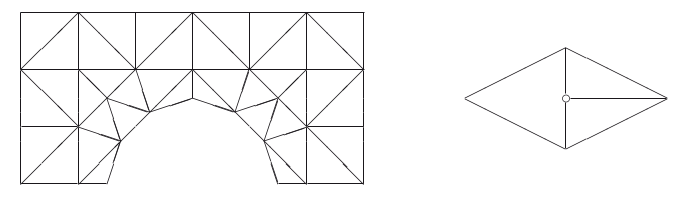
\includegraphics[width=0.8\textwidth]{triangulierung.png} \\
	Abbildung aus \cite{braess2013finite} Seite 58
\end{figure}
Wir werden außerdem im Laufe der Thesis dazu übergehen, ähnlich wie bereits im Abschnitt über die Multilevel Monte Carlo Methode auch bei Zerlegungen von 'Leveln' zu sprechen. Dabei betrachten wir stets eine uniforme Familie zulässiger Zerlegungen $ \{\mathcal{T}_h\}_{h \in \mathcal{H}} $ und fordern dabei, dass die Indexmenge $ \mathcal{H} $ eine ganz bestimmte Form hat. Genauer soll \[ \mathcal{H} = \{ h_0 , h_1 \coloneqq \frac{h_0}{2},h_2 \coloneqq \frac{h_1}{2} = \frac{h_0}{4}, \dots \}  \text{ für ein }  h_0 > 0  \] gelten. Insbesondere gelte also $ \overline{\mathcal{H}} \ni 0 $. Sprechen wir dann von Level $ i $ meinen wir damit die Zerlegung $\mathcal{T}_{h_i} \in \{\mathcal{T}_h\}$.
Zudem führen wir für alle Zerlegungen folgende Bezeichnungen ein:
\begin{itemize}
	\item ein $ K \in \mathcal{T} $ nennen wir Zelle
%	\item $ \mathcal{D}_h \coloneqq \bigcup_{K \in \mathcal{T}} K $ sei die Menge der Zellen
	\item ein $ z \in \mathcal{V}_K \coloneqq \{ z_{K,0} , z_{K,1} , z_{K,2}, z_{K,3}\} \subset \R^2 $ nennen wir Knoten und $\mathcal{V}_K$ die Menge der Knoten von K
	\item $ \mathcal{V}_{\mathcal{T}} \coloneqq \bigcup_{K \in \mathcal{T}} \mathcal{V}_K $ sei die Menge aller Knoten
	\item $\mathcal{F}  \coloneqq (\{ \partial K_1 \cap \partial K_2 : K_1,K_2 \in \mathcal{T} \} \cup \{ \partial K_1 \cap \partial \mathcal{D} : K_1 \in \mathcal{T} \}) \setminus \{\emptyset\} $ sei die Menge aller Seiten
	\item $ \mathcal{F}_K \coloneqq (\{ \partial K \cap \partial K' : K' \in \mathcal{T} \} \cup \{ \partial K \cap \partial \mathcal{D} \}) \setminus \{ \emptyset \} $ sei die Menge aller Seiten von K 
	\item $ \partial \mathcal{D}_h \coloneqq \bigcup_{F \in \mathcal{F}} F $ sei der Rand von $ \mathcal{D}_h $.
\end{itemize}

\subsubsection{Schwache Formulierung}
Betrachten wir also die deterministische Version des Potentialströmungsproblem:
\[ \text{Bestimme } u:\overline{\mathcal{D}} \to \R \text{ und } q: \overline{\mathcal{D}} \to \R^2 \text{ mit } \newline \]
\[\setlength\arraycolsep{1pt}
\text{(PS)}\begin{cases} 
\begin{array}{rlcr}
\dive q     &= 0                 &\text{ ,} \text{in } \mathcal{D} &(1)\\
q           &= - \kappa \nabla u &\text{ ,} \text{in }\mathcal{D} &(2)\\
u           &= u_D               &\text{ ,} \text{auf } \Gamma_D \\
-q \cdot n  &= g_N               &\text{ ,} \text{auf } \Gamma_N 
\end{array}
\end{cases} 
\]
Satz \ref{testfunktionen} sagt uns , dass wir in obiger Formulierung Gleichung (1) mit Testfunktionen $\phi \in H^1(\mathcal{D})$ und Gleichung (2) mit Testfunktionen $\psi \in H^1(\dive,\mathcal{D})$ multiplizieren und anschließend über $\mathcal{D}$ integrieren können und so eine äquivalente schwache Formulierung herleiten:
\begin{align*}
	\int_{\mathcal{D}} \dive(q) \phi \dx &= 0 \text{ für alle Testfunktionen } \phi : \mathcal{D} \to \R \\
	\int_{\mathcal{D}} (q + \kappa \nabla u) \cdot \psi \dx &= 0 \text{ für alle Testfunktionen } \psi : \mathcal{D} \to \R^2
\end{align*}
Da $\kappa$ weiter symmetrisch positiv definit ist, lässt sich letztere Gleichung zu 
\begin{align*}
	&\int_{\mathcal{D}} \kappa^{-1} (q + \kappa \nabla u) \cdot \psi \dx = 0 \\
	\Leftrightarrow \qquad &\int_{\mathcal{D}} \nabla u \cdot \psi \dx = - \int_{\mathcal{D}} (\kappa^{-1}q)\cdot \psi \dx \qquad (\star) 
\end{align*}
umformen. Außerdem wollen wir nun noch die Dirichlet-Randbedingungen $u = u_D \text{ auf } \Gamma_{\text{D}}$ einfließen lassen. Dazu verwenden wir den Satz von Gauß:


\[ \int_{\partial\Omega} (u\psi) \cdot n \da \stackrel{\text{Gauß}}{=} 
 \int_{\Omega} \dive(u\psi) \dx = \int_{\Omega} \nabla u \cdot \psi \dx + \int_{\Omega} u \dive(\psi) \dx \quad (\psi:\Omega \to \R^2) \]
Wählen wir nun unseren Ansatzraum so, dass  für die Funktion $ \psi$ gilt $ \psi \cdot n = 0 \text{ auf } \Gamma_N $. Damit folgt
\begin{align*}
\int_{\Gamma_D} (u_D\psi) \cdot n \da \overset{\psi \cdot n|_{\Gamma_N} = 0}{\underset{u |_{\Gamma_D} = u_D} {=}} \int_{\partial\Omega} (u\psi) \cdot n \da = \underbrace{\int_{\Omega} \nabla u \cdot \psi \dx}_{\stackrel{(\star)}{=}- \int_{\Omega} (\kappa^{-1} q) \cdot \psi \dx } + \int_{\Omega} u \dive(\psi) \dx.
\end{align*}
Die Neumann-Randbedingung $ (\kappa\nabla u) \cdot n = g_N \text{ auf } \Gamma_N $ wird durch die Wahl des Lösungsraumes erfüllt.


Wir erhalten so folgende schwache Formulierung:
\label{sPS}
\begin{align*}
&\text{Bestimme } (q,u) \text{ mit } q\cdot n = -g_N \text{ auf } \Gamma_N \text{ und}\\
&\text{(sPS)}\begin{cases}
\begin{array}{llll}
\int_{\mathcal{D}} \kappa^{-1} q \cdot \psi \dx \, - \mkern-15mu &\int_{\mathcal{D}} u \, \dive(\psi) \dx &= - \int_{\Gamma_D} (u_D \psi) \cdot n \da\\
&\int_{\mathcal{D}} \dive(q) \, \phi \dx &= 0
\end{array}
\end{cases}	\\
&\text{ für alle } (\psi, \phi) \text{ in einem geeigneten Testraum mit } \psi \cdot n = 0 \text{ auf } \Gamma_N 
\end{align*}

\subsubsection{Diskretisierung}
Sei $\mathcal{T}  $ eine zulässige Zerlegung von $ \mathcal{D} $ und alle Bezeichnungen wie oben.
Dabei sei im Weiteren $ N \coloneqq \abs{\mathcal{F}} $ die Anzahl der Seiten und $M = \abs{\mathcal{T}}$ die Anzahl der Zellen.
Wir nummerieren zunächst die Zellen und die Seiten durch:
\begin{align*}
	\mathcal{F} &= \{ F_1,\dots,F_{N}\} \qquad \text{globale Seitennummerierung} \\
	\mathcal{T} &=  \{ K_1,\dots,K_{M}\} \qquad \text{globale Zellennummerierung}
\end{align*}
Als Nächstes soll es nun Ziel sein, eine Lösung der im letzten Abschnitt erklärten schwachen Formulierung in einem endlich dimensionalen Finite Elemente Ansatzraum zu bestimmen. Um aber hierfür genau diese Räume definieren zu können, benötigen wir zuerst sogenannte Basisfunktionen, genauer die Seiten- und die Zellenbasis.\\

 \begin{Definition}(Seiten- und Zellenbasis) 
	\begin{enumerate}[label=(\alph*)]
		\item $ \{ \psi_i \}_{i=1}^{N} $ heißt Seitenbasis und ist definiert durch
			\begin{align*}
					\forall i,j \in \{1, \dots , N \} : \int_{F_j} \psi_i \cdot n^K \da = \pm \delta_{i,j} \text{ und }  \psi_i|_K \in \mathbb{P}_1(K,\R^2) \cap C(\overline{\mathcal{D}}) \ (K \in \mathcal{T}) 
			\end{align*} 
		\item $ \{ \mu_i \}_{i=1}^{M} $ heißt Zellenbasis und ist gegeben durch
			\begin{align*}
				\forall i \in \{1, \dots , M \} : \mu_i \coloneqq  \mathds{1}_{K_i}.
			\end{align*}
	\end{enumerate}
\end{Definition} 

Anschließend können wir mithilfe dieser Basisfunktionen die Testräume bzw. Finite Elemente Räume definieren:
\begin{Definition}(Ansatzräume)
	\begin{enumerate}[label=(\alph*)]
		\item $ W_h \coloneqq \spann \{ \psi_1,\dots,\psi_{N}\}$ (Seitenansatzraum/ Raum für $ \psi $ und $ q_h $)
		\item $ W_h(g) \coloneqq \{ \psi_h \in W_h:  \int_F \psi_h \cdot n \da = \int_F g \da \; \text{ für alle } F \subseteq \Gamma_{\text{N}})  \}$
		\item $ \mathcal{Q}_h \coloneqq \spann \{ \mu_1, \dots, \mu_{M} \} $ (Zellenansatzraum/ Raum für $\phi $ und $ u_h $)
	\end{enumerate}
\end{Definition}

%\begin{Bemerkung}
%	
%	\[	\forall K \in \mathcal{K}:\psi_i|_K \in \mathbb{P}_1(K,\R^2) \text{ und } \mu_m|_K \in \mathbb{P}_0(K,\R) \]
%	Also
%	\begin{align*}	
%	W_h &\subseteq \prod_{K \in \mathcal{K}} \mathbb{P}_1(K,\R^2) &&\text{(Menge der zellenweisen linearen Funktionen) und }\\
%	Q_h &\subseteq \prod_{K \in \mathcal{K}} \mathbb{P}_0(K,\R) &&\text{(Menge der zellenweisen konstanten Funktionen)}. 
%	\end{align*}	
%\end{Bemerkung}

Zusammen mit der schwachen Formulierung \eqref{sPS} erhalten wir so das nun diskretisierte Problem:
\begin{align*}
&\text{Bestimme } (q_h,u_h) \in W_h(-g_N) \times \mathcal{Q}_h \text{ mit}\\
&\begin{cases}
\begin{array}{llll}
\int_{\Omega} \kappa^{-1} q_h \cdot \psi_h \dx \, - \mkern-15mu &\int_{\Omega} u_h \, \dive(\psi_h) \dx &= - \int_{\Gamma_D} (u_D \psi_h) \cdot n \da\\
&\int_{\Omega} \dive(q_h) \, \phi_h \dx &= 0
\end{array}
\end{cases}	\\
&\text{ für alle } (\psi_h, \phi_h) \in W_h(0) \times \mathcal{Q}_h
\end{align*} 




\subsection{Formulierung als LGS}
%Es seien wie bisher Seiten, Seitenbasis, Zellen und Zellenbasis global nummeriert 
%\begin{align*}
%&N \coloneqq \abs{\mathcal{F}} &&\mathcal{F} = \{F_1, \dots , F_{N} \}  \\
%&&&W_h =\{\psi_1, \dots , \psi_N\}\\
%&M \coloneqq \abs{\mathcal{K}} &&\mathcal{K} = \{K_1, \dots , K_{M} \}  \\
%&&&Q_h = \{\mu_1 , \dots , \mu_M  \}.
%\end{align*}

Wir können nun damit beginnen, das so entstandene endlich dimensionale Problem in ein Lineares Gleichungs System umzuformulieren. Dazu definieren wir:
	\begin{align*}
	&\underline{A} \in \R^{N \times N} \text{ mit } \underline{A}[n,k] \coloneqq \int_{\Omega} \kappa^{-1} \psi_n \cdot \psi_k \dx \\
	&\underline{B} \in \R^{M \times N} \text{ mit } \underline{B}[m,k] \coloneqq - \int_{\Omega} \mu_m \dive(\psi_k) \dx \\
	&\underline{b} \in \R^N \text{ mit } \underline{b}[k] \coloneqq - \int_{\Gamma_D} u_D \psi_k \cdot n \da
	\end{align*}
	und (für die Randbedingungen)
	\begin{align*}
	\underline{W}(g) \coloneqq \left\{ \underline{q} \in \R^N : \underline{q}[k] = \int_{F_k} g  \da \ (\text{für } k \text{ mit } F_k \subseteq \Gamma_N) \right\} 
	\end{align*}


Unser zu lösendes Problem lässt sich so mit $ q_h = \sum_{n=1}^{N} \underline{q}[n] \psi_n $ und $ u_h = \sum_{m=1}^{M} \underline{u}[m] \mu_m $ umformen zu 
\begin{align*}
\text{Bestimme} (\underline{q},\underline{u}) \in \underline{W}(-g_N)\times \R^{M} \text{ mit }\\
\begin{cases}
\underline{A} \underline{q} + \underline{B}^T \underline{u} &= \underline{b} \\
\underline{B} \underline{q} &= 0
\end{cases}
\end{align*}
oder anders geschrieben 
\begin{align*}
\text{Bestimme} (\underline{q},\underline{u}) \in \underline{W}(-g_N)\times \R^{M} \text{ mit }\\
\begin{cases}
\begin{pmatrix}
\underline{A} &\underline{B}^T\\
\underline{B} &0
\end{pmatrix}
\begin{pmatrix}
\underline{q} \\
\underline{u} 
\end{pmatrix}
=
\begin{pmatrix}
\underline{b}\\
0
\end{pmatrix}.
\end{cases}
\end{align*}

Wir haben so eine diskrete gemischte Formulierung des Potentialströmungsproblems hergeleitet und können mit dieser aus gegebenen Rand- und Anfangswerten ein Flussvektorfeld $q$ erzeugen, welches der obigen Differentialgleichung genügt.
Es handelt sich hierbei um das gemischte Finite Elemente Verfahren. In M++ selbst lösen wir das Potentialströmungsproblem durch eine Abwandlung dieses Verfahrens. Wir diskretisieren dazu eine äquivalente Formulierung von (sPS) und erhalten so mit dem hybriden Finite Elemente Verfahren die gleichen Ergebnisse, die auch der vorgestellte gemischte Ansatz liefern würde, bei besserer Effizienz und guter Parallelisierbarkeit. Da das Potentialströumgsproblem in dieser Thesis primär dazu genutzt werden soll, das Vektorfeld $q$ zu bestimmen, soll uns aus theoretischer Sicht aber obige Formulierung genügen und wir verweisen hinsichtlich der Lösung mit hybriden gemischten Finiten Elementen, neben einem kleinen, Überblick verschaffendem Abschnitt im Appendix \ref{Referenzzelle&Hyb}, auf die Literatur, wie etwa \cite{brezzi2012mixed} oder  \cite{roberts1991mixed}.












%%%%%%%%%%%%%%%%%%%%%%%%%%%%%%%%%
\newpage  % neuer Abschnitt auf neue Seite, kann auch entfallen
%%%%%%%%%%%%%%%%%%%%%%%%%%%%%%%%%
\subsection{Numerische Lösung des Transportproblems}
% !TeX root = bachelorarbeit.tex
 \label{DG}
In diesem Abchnitt soll nun, nachdem wir $q(\omega,\cdot)$ als Finite-Elemente-Lösung des Potentialströmungsproblems erhalten haben, die numerische Lösung des linearen Transportproblems behandelt werden:
\begin{align*}
	&\text{Für } \omega \in \Omega \text{ und }q(\omega,\cdot): \overline{\mathcal{D}} \to \R^2 \text{, bestimme }\rho(\omega,\cdot): \overline{\mathcal{D}} \times \mathbb{T} \to \R_{\geq 0} \text{ mit} \\
	&\text{(pTP)} 
	\begin{cases}
	\begin{array}{rlll}
	\partial_t \rho (\omega, x, t) + \dive(\rho(\omega,x,t)q(\omega,x)) &= 0 &\text{, für } (x,t) \in \mathcal{D} \times (0,T] \\
	\rho(\omega,x,t) &= \rho_{\text{in}}(x,t) &\text{, für } (x,t) \in \Gamma_{\text{in}} \times \mathbb{T} \\
	\rho(\omega,x,0)  &= \rho_0(x) &\text{, für } x \in  \mathcal{D}
	\end{array}
	\end{cases} \\
\end{align*}
Insbesondere wollen wir an dieser Stelle wieder $\omega \in \Omega$ festhalten und betrachten deshalb zunächst nur das deterministische Problem wie in \ref{det_prob}:
\[ 
\text{Bestimme } \rho: \overline{\mathcal{D}} \times \mathbb{T} \to \R_{\geq 0} \text{, sodass} \newline \]
\[\setlength\arraycolsep{1pt}
\text{(dTP)}\begin{cases} 
\begin{array}{rlll}
\partial_t \rho(x,t) + \dive(\rho(x,t) q(x)) &= 0 &\text{ ,in } &\mathcal{D} \times (0,T)\\
\rho(x,t) &= \rho_{\text{in}}(x,t) &\text{ ,auf } &\Gamma_{\text{in}} \times (0,T)\\
\rho(x,0) &= \rho_0(x) &\text{ ,auf } &\mathcal{D} \\
\end{array}
\end{cases} \\
\]
 Wir greifen dabei auf ein sogenanntes discontinuous Galerkin Verfahren zurück, welches für diese Problemklasse bereits an anderen Stellen (z.B. in \cite{cockburn1998runge}) erprobt wurde. Ursprünglich geht das Discontinuous Galerkin Verfahren auf Reed und Hill \cite{reed1973triangular} zurück. Einen guten (wenn auch mittlerweile etwas in die Jahre gekommenen) Überblick über die Anwendung von discontinuous Galerkin Verfahren bietet \cite{cockburn2000development}.
Grundätzlich handelt es sich beim discontinuous Galerkin Verfahren ebenfalls um einen FEM Ansatz, der zwar Ähnlichkeiten zum Finite Elemente Verfahren aufweist, welches wir im letzten Abschnitt gesehen hatten, aber auch einige bedeutende Unterschiede besitzt, auf welche wir im Folgenden besonders eingehen wollen. 
%So werden wir wieder eine schwache Formulierung des analytischen Problems herleiten und uns dann im Rahmen des diskretisierung erneut auf endlich dimensionale Räume zurückziehen.
Anders als zuvor das Potentialströmungsproblem ist die lineare Transportgleichung  nämlich sowohl orts- als auch zeitabhängig. Daher werden wir
%, nachdem wieder zuerst eine schwache Formulierung eingeführt wird,
  die lineare Transportgleichung zunächst im Ort diskretisieren. Wir erhalten so eine Semidiskretisierung, welche wir anschließend mit einem Zeitintegrator, wie beispielsweise der impliziten Mittelpunktsregel, in eine Volldiskretisierung überführen.
 

%\subsubsection{Schwache Formulierung}
%Wie im letzten Abschnitt führen wir nun einen schwachen Lösungsbegriff ein. Sei dazu $ \phi : \mathcal{D} \times \mathbb{T} \to \R $ eine beliebige Testfunktion, etwa aus  $W_0^{1,2}(\mathcal{D} \times \mathbb{T}) $, für die $ \phi(\cdot,T) = 0 $ gelte. 
%Wir beginnen mit der differentialgleichung $ \partial_t \rho(x,t) + \dive(\rho(x,t) q(x)) = 0  $, multiplizieren zunächst mit der Testfunktion $ \phi $ und integrieren anschließend über den Raum-Zeitzylinder $ \mathcal{D} \times \mathbb{T} $:
%\begin{align*}
%	\int_{\mathcal{D} \times \mathbb{T}} \big(\partial_t \rho(x,t) &+ \dive(\rho(x,t) q(x) ) \big) \phi(x,t) \; \mathrm{d} (x,t) =  \\
%	&\underbrace{\int_{\mathcal{D} \times \mathbb{T}}  \partial_t \rho(x,t) \phi(x,t) \; \mathrm{d} (x,t)}_{(1)} +\underbrace{\int_{\mathcal{D} \times \mathbb{T}}  
%    \dive(\rho(x,t) q(x) ) \phi(x,t)\; \mathrm{d} (x,t)}_{(2)}
%\end{align*}
%Betrachten wir nun zunächst Integral (1), so folgt mit partieller Integration:
%\begin{align*}
%	\int_{\mathcal{D} \times \mathbb{T}}  \partial_t \rho(x,t) &\phi(x,t) \; \mathrm{d} (x,t) = \int_{\mathcal{D}} \int_{\mathbb{T}} \partial_t \rho(x,t) \phi(x,t) \dt \dx \\&= \int_{\mathcal{D}} \big( - \int_{\mathbb{T}} \rho(x,t) \partial_t \phi(x,t) \dt + \big[ \rho(x,t) \phi(x,t) \big]_0^T  \big) \dx \\
%	&= - \int_{\mathcal{D} \times \mathbb{T}} \rho(x,t) \partial_t \phi(x,t) \; \mathrm{d} (x,t) + \int_{\mathcal{D}} \underbrace{\rho(x,T) \phi(x,T)}_{ = 0 } - \underbrace{\rho(x,0)}_{ = \rho_0(x) \text{ auf } \mathcal{D}} \phi(x,0)  \dx\\
%	&= - \int_{\mathcal{D} \times \mathbb{T}} \rho(x,t) \partial_t \phi(x,t) \; \mathrm{d} (x,t) - \int_{\mathcal{D}} \rho_0(x) \phi(x,0) \dx 
%\end{align*}
%Außerdem können wir Integral (2) mit  \ref{n_pI} wie folgt ausdrücken:
%\begin{align*}
%	\int_{\mathcal{D} \times \mathbb{T}}  
%	\dive(\rho(x,t) &q(x) ) \phi(x,t)\; \mathrm{d} (x,t) = \int_{\mathbb{T}} \int_{\mathcal{D}} \dive(\rho(x,t) q(x) ) \phi(x,t) \dx \dt \\
%	&= \int_{\mathbb{T}} \big( - \int_{\mathcal{D}} \rho(x,t) q(x) \nabla \phi(x,t) \dx + \int_{\partial \mathcal{D}} \rho(x,t) q(x) \cdot n \ \phi(x,t) \da \big)  \dt \\
%	&= - \int_{\mathcal{D} \times \mathbb{T}} \rho(x,t) q(x) \nabla \phi(x,t)) \; \mathrm{d} (x,t) + \int_{\mathbb{T}} \int_{\partial \mathcal{D}} \rho(x,t) q(x) \cdot n \phi(x,t) \da \dt 
%\end{align*}
%Mit $ \partial \mathcal{D} = \Gamma_{\text{in}} \dot{\cup} \Gamma_{\text{out}} $ und 
%$\rho(x,t) = \rho_{\text{in}}(x,t) \text{ für } (x,t) \in \Gamma_{\text{in}} \times (0,T)$ erhalten wir so die folgende Formulierung:
%\begin{definition} 
%$ \rho \in L_1 (\mathcal{D} \times (0,T)) $ heißt schwache Lösung des linearen Transportproblems, falls es für ein gegebenes $ q : \overline{\mathcal{D}} \to \R^2 $ folgende Bedingungen erfüllt:
%\begin{align*}
%\text{(swTP)}
%\begin{cases}
%\begin{array}{rlll}
%\displaystyle
%\int_{\mathcal{D}} \rho_0 \phi(0) \dx = \mkern-16mu &- \displaystyle \int_{0}^{T} \int_{\mathcal{D}} \rho (\partial_t \phi + q \nabla \phi ) \dx \dt \\
%&+\displaystyle\int_{0}^{T}  \int_{\Gamma_{\text{in}}} \rho_{\text{in}} q \cdot n \phi \da  \dt \\
%&+\displaystyle\int_{0}^{T}  \int_{\Gamma_{\text{out}}} \rho q \cdot n \phi \da  \dt
%\end{array}
%\end{cases}	
%\end{align*}
%für alle Testfunktionen $ \phi: \mathcal{D} \times (0,T) \to \R $ mit $ \phi(\cdot,T) = 0 $ auf $ \mathcal{D}  $ und $ \phi|_{\Gamma_{\text{out}}} = 0 $.
%\end{definition}
%dabei ist $  \Gamma_{\text{out}} \coloneqq  \{ z \in \partial \mathcal{D}: q(z)\cdot n(z) > 0 \}$ 
%und $  \Gamma_{\text{in}} \coloneqq  \{ z \in \partial \mathcal{D}: q(z)\cdot n(z) \leq 0 \} $. \\
%Obige Herleitung zeigt zusammen mit \ref{testfunktionen} insbesondere die Gültigkeit des folgenden Zusammenhangs zwischen klassischen Lösungen der linearen Transportgleichung und schwachen Lösungen von (swTP):
%
%\begin{Lemma}(Zusammenhang der Lösungsbegriffe)
%	\begin{enumerate}
%		\item Ist $ \rho $ eine klassische Lösung, so ist $ \rho $ auch eine schwache Lösung.
%		\item Ist $ \rho \in C^2(\mathcal{D} \times \mathbb{T} , \R )$ und eine schwache Lösung, so ist $ \rho $ auch eine klassische Lösung. 
%	\end{enumerate}
%\end{Lemma}
\subsubsection{Diskretisierung}
\label{Diskretisierung}
Wie bereits weiter oben beschrieben, werden wir im Folgenden zunächst den Raum diskretisieren und anschließend die so entstandene Semidiskretisierung in eine Volldiskretisierung auflösen. Insgesamt wollen wir das discontinuous Galerkin Verfahren mit einem Zeitintegrator, wie der impliziten Mittelpunktsregel oder einem klassischen Runge-Kutta-Verfahren nutzen. Zunächst führen wir die analytische Flussfunktion ein. 
\begin{Definition}(Flussfunkion) \\
	\label{Flussfunktion}
	Zu einem gegebenen Flussvektorfeld $ q : \mathcal{D} \to \R^2 $ ist die Flussfunktion $ \Upsilon$ definiert als:\\
	\begin{align*}
		 \Upsilon : \text{Abb}(\mathcal{D}\times\mathbb{T},\R) &\to \text{Abb}(\mathcal{D}\times\mathbb{T},\R^2) \\
		 \rho &\mapsto \rho q
	\end{align*}
\end{Definition}
$\newline$
Für eine klassische Lösung $ \rho  $ von (dTP) gilt dann insbesondere $ \partial_t \rho = - \dive (\Upsilon(\rho)) $ auf $ \mathcal{D} \times (0,T] $.	\\
Halten wir also zunächst $ t \in \mathbb{T} $ und leiten so die Semidiskretisierung her.\\
Sei nun $ \mathcal{T} $ eine zulässige Triangulierung von $ \mathcal{D} $ aus Dreiecken wie in \ref{num_pot} und  $ (\cdot , \cdot)_A $ das $ L^2(A)-$Skalarprodukt.
Wir wählen als Lösungs-/Testraum $\mathcal{Q}_h = \prod_{K \in \mathcal{T}} \mathbb{P}_p(K,\R) $ für ein festes $p \geq 1 $. Anders als zuvor fordern wir für unsere Lösungs- und Testfunktionen diesmal aber \underline{nicht} die Stetigkeit auf $\mathcal{D}$. Da so $\mathcal{Q}_h$ nicht im betrachteten analytischen Lösungs- und Testraum liegt, etwa  $\mathcal{Q}_h \nsubseteq H^1(\mathcal{D})$, nennt man $\mathcal{Q}_h$ auch einen nicht-konformen Ansatzraum.
Außerdem lässt sich im Allgemeinen auch die später bestimmte Lösung $ \rho_h \in \mathcal{Q}_h $ (definiert auf $\mathcal{D}_h = \bigcup_{K \in \mathcal{T}} K$ ) nicht stetig auf $ \mathcal{D} $ fortsetzen, denn für eine beliebige innere Kante $ F $ kann der Grenzwert von $ \rho_h $ auf den anliegenden Zellen $ K,K' $ ($ \overline{F} = \partial K \cap \partial K' $) unterschiedlich sein. \\
Trotzdem müssen wir auch auf den inneren Kanten $ \mathcal{F}^0 \subset \mathcal{F} $ festlegen, welcher Grenzwert in einem solchen Falle gewählt wird. \\
Dazu führen wir als Pendant zur analytischen Flussfunktion (vgl. \ref{Flussfunktion})
auch eine numerische Flussfunktion ein. Grundsätzlich kommen mehrere solche Flussfunktionen in Frage, welche direkten Einfluss auf Eigenschaften des entstehenden Verfahrens besitzen. Wir entscheiden uns an dieser Stelle für den weit verbreiteten 
sogenannten upwind flux:
\begin{Definition}(upwind flux)\\
	Sei $K \in \mathcal{T}$ eine beliebige Zelle und $ F \in \mathcal{F}_K$ eine Kante von $K$. Dann ist
	\begin{align*}
		\Upsilon^{\star} : \text{Abb}(\mathcal{D}\times\mathbb{T},\R) &\to \text{Abb}(\mathcal{D}\times\mathbb{T},\R^2) \\
		\rho_h &\mapsto 
		\begin{cases}
			\Upsilon(\rho_h|_K) , \ \text{ für } q\cdot n_F^K \geq 0 \\  
			\Upsilon(\rho_h|_{K'}) ,\text{ für } q\cdot n_F^K < 0 \text{ und } \overline{F} = \partial K \cap \partial K'
		\end{cases}
	\end{align*}
\end{Definition}
Sei nun also $ \rho $ klassische Lösung von (dTP) mit $ \partial_t \rho = -\dive(\Upsilon(\rho)) $ auf $ \mathcal{D} $. Dann gilt nach Satz von Gauß:
\begin{align}
		\label{gaus1}
		\int_{\partial \mathcal{D}} \rho q \cdot n \phi \da  =\int_{\partial \mathcal{D}} \Upsilon(\rho) \cdot n \phi \da = \int_{\mathcal{D}} \dive (\Upsilon(\rho)\phi) \dx
\end{align}
Das Integral über den Rand von $ \mathcal{D} $ können wir nach der folgenden kleinen Vorüberlegung auch als Integral über alle Kanten der gewählten Zerlegung $ \mathcal{T} $ ausdrücken: \\
Es gilt nämlich für alle inneren Kanten, also solche Kanten $ F $, für die zwei Zellen $ K $ und $ K' $ existieren, sodass $ \overline{F} = K \cap K' $ ist, dass $ \int_F \Upsilon^{\star}(\rho) \cdot n^K \phi \da = - \int_F \Upsilon^{\star}(\rho) \cdot n^{K'} \phi \da $ stets erhalten ist. \\
Summieren wir also zunächst über alle Zellen, summieren anschließend die Integrale über alle Kanten und ersetzen dabei den analytischen durch den numerischen Fluss, erhalten wir gerade wieder obiges Randintegral. Es gilt also:
\begin{align*}
	\sum_{K\in \mathcal{T}} \sum_{F \in \mathcal{F}_K} \int_F \Upsilon^{\star}(\rho) \cdot n^K \phi \da = \int_{\partial \mathcal{D}} \Upsilon(\rho) \cdot n \phi \da \stackrel{\text{\ref{gaus1}}}{=} \int_{\mathcal{D}} \dive (\Upsilon(\rho)\phi) \dx
\end{align*}
Nach der Produktregel der Divergenz lässt sich das letzte Integral auswerten zu:
\begin{align*}
	 \int_{\mathcal{D}} \dive (\Upsilon(\rho)\phi) \dx = \int_{\mathcal{D}} \phi \dive(\Upsilon(\rho)) + \Upsilon(\rho) \cdot \nabla \phi \dx \stackrel{\text{ Vor.}}{=} - \int_{\mathcal{D}} \partial_t \rho \phi \dx + \int_{\mathcal{D}} \Upsilon(\rho) \cdot \nabla \phi \dx
\end{align*}
Durch Umstellen und das Zusammenfassen der obigen Resultate erhalten wir so: 
\begin{align*}
	\sum_{K \in \mathcal{T}} \int_K \partial_t \rho  \phi \dx = \sum_{K \in \mathcal{T}} \int_K \Upsilon(\rho ) \cdot \nabla \phi \dx - 	\sum_{K\in \mathcal{T}} \sum_{F \in \mathcal{F}_K} \int_F \Upsilon^{\star}(\rho) \cdot n^K \phi \da
\end{align*}
Dabei wurde zusätzlich ausgenutzt, dass es sich bei den Kanten um Nullmengen handelt und wir so das Integral über $ \mathcal{D} $ als Summe der Integrale über alle Zellen auffassen können. Nutzen wir nun noch aus, dass für den Fluss  $\rho(x,t) = \rho_{\text{in}}(x,t)$ für $ x \in \Gamma_{\text{in}} $ gilt, kommen wir so auf 
\begin{align}
	\label{fastfertigsemi}
	\sum_{K \in \mathcal{T}} \int_K \partial_t \rho  \phi \dx = \sum_{K \in \mathcal{T}} \int_K \Upsilon(\rho ) \cdot \nabla \phi \dx - 	\sum_{K\in \mathcal{T}} \left( \sum_{\substack{F \in \mathcal{F}_K \\ F \not\subseteq \Gamma_{\text{in}}}} \int_F \Upsilon^{\star}(\rho) \cdot n^K \phi \da - \sum_{\substack{F \in \mathcal{F}_K \\ F \subseteq \Gamma_{\text{in}}}} \rho_{\text{in}} q \cdot n^K \phi \da \right)
\end{align}
Sei nun $ \mathcal{T} = \{ K_1,\dots , K_N\} , N \coloneqq |\mathcal{T}| $. Die Semidiskretisierung ist motiviert durch (\ref{fastfertigsemi}) und lautet: Bestimme  $\rho_h \in \mathcal{Q}_h$, sodass für alle $ \phi_h \in \mathcal{Q}_h $ gilt:
\begin{align}
	\label{Semidiskretisierung}
	\sum_{i=1}^N (\partial_t \rho_h, \phi_h)_{K_i} &= \sum_{i=1}^{N} \big( (\Upsilon(\rho_h), \nabla \phi_h)_{K_i} - \sum_{\substack{F \in \mathcal{F}_K \\ F \not \subseteq \Gamma_{\text{in}}}}(\Upsilon^{\star}(\rho_h)\cdot n^K,\phi_h)_{F} - (\rho_{\text{in}}q \cdot n^K,\phi_h)_{\partial K_i \cap \Gamma_{\text{in}}} \big)
\end{align}


Durch Einsetzen der Zellenbasis $ \{\mu_i\}_{i=1}^N \subset \mathcal{Q}_h $  und mit $ \supp(\mu_i) \subseteq \overline{K_i} (\ i \in \{1, \dots , N\})$ ergibt sich für alle $\ i \in \{1, \dots , N\}$ : \\
TODOOOOOOOOOOOOOOOO überarbeiten
\begin{align*} 
\left(\partial_t \rho_h, \mu_i  \right)_{K_i}  &= \bigg( \underbrace{(\Upsilon(\rho_h), \nabla\mu_i)_{K_i}}_{=0 \text{, da } \nabla \mu_i = 0} - \sum_{\substack{F \in \mathcal{F}_{K_i} \\ F \not\subseteq \Gamma_{\text{in}}}} \left(\Upsilon^*(\rho_h) \cdot n^{K_i}, \mu_i \right)_{F} - \left(\rho_{\text{in}} q \cdot n^{K_i}, \mu_i \right)_{\partial K_i \cap \Gamma_{\text{in}}} \bigg) \\
\end{align*}
Wir erhalten so folgende Darstellung:
%\begin{align*}
%\left(\partial_t \rho_h, \mu_i  \right)_{K_i} = \bigg( - \sum_{\substack{F \in \mathcal{F}_{K_i}, F \not\subseteq \Gamma_{\text{in}}\\ F \text{ mit }q \cdot n^K_{|F} > 0} } \left(\underbrace{\Upsilon^*(\rho_h)}_{= \rho_{h|K}\, q} \cdot n^{K_i}, \mu_i \right)_{F} - \sum_{\substack{F \in \mathcal{F}_{K_i}, F \not\subseteq \Gamma_{\text{in}}\\ F \text{ mit }q \cdot n^K_{|F} < 0} } \left(\underbrace{\Upsilon^*(\rho_h)}_{= \rho_{h|K'} \, q} \cdot n^{K_i}, \mu_i \right)_{F}\\
% - \left(\rho_{\text{in}} q \cdot n^{K_i}, \mu_i \right)_{\partial K_i \cap \Gamma_{\text{in}}} \bigg)
%\end{align*} 

\begin{align}
\label{DarstellungvorLGS}
\underbrace{\left(\partial_t \rho_h, \mu_i  \right)_{K_i}}_{(\ref{DarstellungvorLGS}.1)} = 
\underbrace{-  \sum_{F \in \mathcal{F}_{K_i} , F \not \subseteq \Gamma_{\text{in}}}\left(\Upsilon^{\star}(\rho_h)\cdot n^{K_i},\mu_i\big)_F \right)}_{(\ref{DarstellungvorLGS}.2)} \underbrace{- \left(\rho_{\text{in}}q\cdot n^{K_i},\mu_i \right)_{\partial K_i \cap \Gamma_{\text{in}}}}_{(\ref{DarstellungvorLGS}.3)}
\end{align}

Zusammen mit der Basisdarstellung von $ \rho_h $ in $\{\mu_i  \}_{i=1}^N$, $ \rho_h = \sum_{i=1}^{N} 
\underline{\rho}[i] \; \mu_i$, und \\
$ \Upsilon^{\star}(\rho_h) = 
\begin{cases} 
\rho_h|_K \ ,\text{falls } q\cdot n^K|_F \geq 0\\
\rho_{h}|_{K'} \ , \text{falls } q\cdot n^K|_F < 0
\end{cases} $ können wir \ref{DarstellungvorLGS} in eine gewöhnliche Differentialgleichung erster Ordnung umformulieren. 
Dazu klammern wir jeweils $ \underline{\rho} $ aus und definieren 
\begin{align*}
&\text{mithilfe von (\ref{DarstellungvorLGS}.1) die Massenmatrix } \underline{M}\in \R^{N \times N} \\  &\qquad \qquad \underline{M}[K,K'] \coloneqq \begin{dcases}
\int_K \abs{\mu_K}^2 \dx & \text{, für } K = K' \\
0 &\text{, sonst}
\end{dcases} \\
&\text{mit (\ref{DarstellungvorLGS}.2) die Flussmatrix } \underline{A}\in \R^{N \times N} \\ &\qquad \qquad \underline{A}[K,K'] \coloneqq \begin{dcases}
- \sum_{\substack{F\in \mathcal{F}_K \\ F \text{ mit } q\cdot n^K_{|F} > 0}} \int_F \mu_K^2 q \cdot n^K \da& \text{, für } K = K' \\
- \int_F \mu_K \mu_{K'} q \cdot n^K \da &\text{, für } q \cdot n^K< 0 \text{ und } \overline{F} = \partial K \cap \partial K'\\
0 &\text{, sonst}
\end{dcases} \\
&\text{und mit (\ref{DarstellungvorLGS}.3) den Lastvektor } \underline{b}\in \R^{N} \\ &\qquad \qquad\underline{b}[K] \coloneqq \int_{\partial K \cap \Gamma_{\text{in}}} \rho_{\text{in}} q \cdot n \da
\end{align*}
So ergibt sich die Differentialgleichung
\begin{align*}
\begin{cases}
\underline{M} \partial_t \underline{\rho}(t) = \underline{A} \underline{\rho}(t) + \underline{b}(t) \\
\underline{\rho}(0) = \underline{\rho_0}
\end{cases}\\
\end{align*}
Da dies nun eine gewöhnliche Differentialgleichung ist, können wir die Lösung 
\begin{align}
 \label{semidisklsg}
 \underline{\rho}(t) = \exp(t \underline{M}^{-1} \underline{A}) \left( \underline{\rho_0} + \int_{0}^{t} \exp(-s\underline{M}^{-1} \underline{A}) \underline{b}(s) \ds \right)
\end{align}
explizit angeben.
Es handelt sich hierbei aber immer noch um eine semidiskrete Formulierung. 
Wir wollen deshalb zuletzt noch auf die Herleitung der Zeitintegratoren eingehen. Diese nutzen wir, um unter Verwendung der oben hergeleiteten Semidiskretisierung die numerische Lösung $ \underline{\rho} $ sowohl orts- al auch zeitdiskret zu berechnen. Der Ansatz leitet sich hierbei direkt aus dem Resultat (\ref{semidisklsg}) ab und besteht aus der 
Integration der Differentialgleichung $\underline{M} \partial_t \underline{\rho} = \underline{A} \underline{\rho} + \underline{b}$ über die Zeit $t$ im Intervall $[t_i, t_{i+1}]$.
Dabei ist $t_i = i \delta t$. Hiermit folgt:
\begin{align*}
\underline{M}\underline{\rho}(t_{i+1}) - \underline{M}\underline{\rho}(t_i) = \int_{t_i}^{t_{i+1}}
\underline{M} \partial_t \underline{\rho}(t) dt =\int_{t_i}^{t_{i+1}} \underline{A} \underline{\rho}(t) + \underline{b}(t) dt.
\end{align*}
Mithilfe der Anwendung verschiedener Quadraturformeln lässt sich daraus ein Runge-Kutta Verfahren herleiten. Über die Rechteckformel 
\begin{align*}
\int_{t_i}^{t_{i+1}}\underline{A} \underline{\rho}(t) + \underline{b} dt \approx (t_{i+1}-t_i)( 
\underline{A} \underline{\rho}(t_{i+1}) + \underline{b}(t_{i+1})) = \delta t (\underline{A} \underline{\rho}(t_{i+1}) + \underline{b}(t_{i+1}))
\end{align*}
ergibt sich z.B. das implizite Euler Verfahren
\begin{align*}
\underline{\rho}(t_{i+1}) = \underline{\rho}(t_{i}) + \delta t \underline{M}^{-1}(\underline{A} \underline{\rho}(t_{i+1}) + \underline{b}(t_{i+1})).
\end{align*}
%Weitere Verfahren, die wir verwenden werden, sind zum einen das
%klassische Runge-Kutta Verfahren (der Übersicht wegen für $\underline{b} \equiv 0$)
%\begin{align*}
%\underline{\rho}(t_{i+1}) = \underline{\rho}(t_{i}) +
%\delta t \underline{M}^{-1}\underline{A} (
%\underline{\rho}(t_{i}) +
%\frac{\delta t}{2} \underline{M}^{-1}\underline{A} (
%\underline{\rho}(t_{i}) +
%\frac{\delta t}{3} \underline{M}^{-1}\underline{A} (
%\underline{\rho}(t_{i}) +
%\frac{\delta t}{4} \underline{M}^{-1}\underline{A} 
%\underline{\rho}(t_{i}) )))
%\end{align*}
%und zum anderen die implizite Mittelpunktsregel 
Ein weiteres Verfahren dieser Art, welches wir an dieser Stelle verwenden werden, ist die implizite Mittelpunktsregel (der Übersicht wegen für $\underline{b} \equiv 0$):
\begin{align*}
\underline{\rho}(t_{i+1}) = \underline{\rho}(t_{i}) +
\delta t \underline{M}^{-1} (
\underline{A} 
\frac{1}{2}(\underline{\rho}(t_{i}) +
\underline{\rho}(t_{i+1}) )
+
\frac{1}{2} ( \underline{\rho}(t_{i}) +
\underline{\rho}(t_{i+1}) )).
\end{align*}

Das so entstehenden Gesamtverfahren ist aufgrund der Kombination von Discontinuous Galerkin Verfahren und Runge-Kutta-Zeitintegratoren in der Literatur oft auch unter dem Namen 'Runge–Kutta discontinuous Galerkin Methods' zu finden. Einen schönen Überblick über diese Verfahrensklasse bietet der Artikel \cite{cockburn2001runge}.
Nachdem wir nun das Discontinuous Galerkin Verfahren für die lineare Transportgleichung eingeführt und erklärt haben, sollen nun noch auf einige Eigenschaften des Verfahrens verwiesen werden. Dabei wollen wir uns aber beschränken, einige grundlegende Resultate zu nennen und so eher einen groben Überblick mit Referenzen zur Literatur zu geben. Mehr zur numerischen Analyse des Discontinuous Galerkin Verfahren findet sich zum einen in Standardwerken, wie \cite{ern2004theory}, eine schöne Zusammenstellung bietet aber auch
\cite{Har08b}. \\
Ebenfalls findet sich in \cite{Har08b} eine grundlegende numerische Analyse des Discontinuous Galerkin Verfahrens angewandt auf die stationäre lineare Transportgleichung. Dabei werden unter anderem die Konsistenz, die sogenannte Galerkin-Orthogonalität, sowie die Stabilität und Konvergenz des Verfahrens behandelt.
Mit der numerischen Analyse des Discontinuous Galerkin Verfahrens an sich befassten sich unter anderem LeSaint und Raviart \cite{lesaint1974finite}, Peterson \cite{peterson1991note} und Richter \cite{richter1988optimal}.
Runge-Kutta DG Verfahren für der linearen Transportgleichung ähnliche Problemstellungen betrachteten Cockburn und Shu in einer 5-teiligen Serie von Arbeiten. Besonders zu nennen sind dabei in unserem Kontext \cite{cockburn1989tvb} und \cite{cockburn1990runge}.


\subsection{Eigenschaften des Discontinuous Galerkin Verfahren}
Nachdem wir nun das Discontinuous Galerkin Verfahren für die lineare Transportgleichung eingeführt und erklärt haben, sollen noch einige Eigenschaften des Verfahrens beleuchtet werden. Dabei wollen wir uns aber darauf beschränken, einige grundlegende Resultate zu nennen, und so eher einen groben Überblick mit Referenzen zur Literatur zu geben. Mehr zur numerischen Analyse des Discontinuous Galerkin Verfahren findet sich zum einen in Standardwerken, wie \cite{ern2004theory}, eine schöne Zusammenstellung bietet aber auch \cite{Har08b}.
Ebenfalls findet sich in \cite{Har08b} eine grundlegende numerische Analyse des Discontinuous Galerkin Verfahrens auf die stationäre lineare Transportgleichung.
\subsubsection{Lösungsbegriffe}
	Wie zuvor bereits beim Potentialströmungsproblem können wir auch für das Transportproblem eine sogenannte schwache Formulierung bestimmen. Diese hängt im Fall des Transportproblems eng mit der Semidiskretisierung zusammen und lautet mit $ \partial \mathcal{D} = \Gamma_{\text{in}} \dot{\cup} \Gamma_{\text{out}} $ und 
$\rho(x,t) = \rho_{\text{in}}(x,t) \text{ für } (x,t) \in \Gamma_{\text{in}} \times (0,T)$ :
\begin{Definition} 
	$ \rho \in L_1 (\mathcal{D} \times (0,T)) $ heißt schwache Lösung des linearen Transportproblems, falls es für ein gegebenes $ q : \overline{\mathcal{D}} \to \R^2 $ folgende Bedingungen erfüllt:
	\begin{align*}
	\begin{array}{rllll}
	&\text{(swTP)} \ &B(\rho,\phi) &= \langle b,\phi\rangle \quad \forall \phi \in H^1(\mathcal{D}\times\mathbb{T}) \text{ mit } \phi(\cdot,T) = 0 \text{ und } \phi|_{\Gamma_{\text{out}}} = 0 \\
	&\text{Dabei sind :} & & &\\
	& &B(\rho,\phi) &\coloneqq  \int_{0}^{T} \int_{\mathcal{D}} \rho (\partial_t \phi + q \nabla \phi ) \dx \dt - \int_{\Gamma_{\text{out}}} \rho q \cdot n \phi \da  \dt \\
	& &\langle b,\phi \rangle &\coloneqq \int_{\Gamma_{\text{in}}} \rho_{\text{in}} q \cdot n \phi \da  \dt - \int_{\mathcal{D}} \rho_0 \phi(0) \dx \\
	& & \Gamma_{\text{out}} &\coloneqq  \{ z \in \partial \mathcal{D}: q(z)\cdot n(z) > 0 \} & \\
	& & \Gamma_{\text{in}} &\coloneqq  \{ z \in \partial \mathcal{D}: q(z)\cdot n(z) \leq 0 \} &
	\end{array}\\
	%		\text{(swTP)}
	%		\begin{cases}
	%		\begin{array}{rlll}
	%		\displaystyle
	%		\int_{\mathcal{D}} \rho_0 \phi(0) \dx = \mkern-16mu &- \displaystyle \int_{0}^{T} \int_{\mathcal{D}} \rho (\partial_t \phi + q \nabla \phi ) \dx \dt \\
	%		&+\displaystyle\int_{0}^{T}  \int_{\Gamma_{\text{in}}} \rho_{\text{in}} q \cdot n \phi \da  \dt \\
	%		&+\displaystyle\int_{0}^{T}  \int_{\Gamma_{\text{out}}} \rho q \cdot n \phi \da  \dt
	%		\end{array}
	%		\end{cases}	
	\end{align*}
	%		für alle Testfunktionen $ \phi: \mathcal{D} \times (0,T) \to \R $ mit $ \phi(\cdot,T) = 0 $ auf $ \mathcal{D}  $ und $ \phi|_{\Gamma_{\text{out}}} = 0 $.
\end{Definition}
%	dabei ist $  \Gamma_{\text{out}} \coloneqq  \{ z \in \partial \mathcal{D}: q(z)\cdot n(z) > 0 \}$ 
%	und $  \Gamma_{\text{in}} \coloneqq  \{ z \in \partial \mathcal{D}: q(z)\cdot n(z) \leq 0 \} $. \\
%	

Es gilt an dieser Stelle außerdem:

\begin{Lemma}(Zusammenhang der Lösungsbegriffe)
	\begin{enumerate}
		\item Ist $ \rho $ eine klassische Lösung, so ist $ \rho $ auch eine schwache Lösung.
		\item Ist $ \rho \in C^2(\mathcal{D} \times \mathbb{T} , \R )$ und eine schwache Lösung, so ist $ \rho $ auch eine klassische Lösung. 
	\end{enumerate}
\end{Lemma}

\begin{proof}
	Sei $ \phi : \mathcal{D} \times \mathbb{T} \to \R $ eine beliebige Testfunktion aus  $H^1(\mathcal{D} \times \mathbb{T}) $, für die $ \phi(\cdot,T) = 0 $ und $ \phi|_{\Gamma_{\text{out}}} = 0 $ gelte. Wir halten zunächst fest, dass der Raum $ H_0^1(\mathcal{D} \times \mathbb{T}) $ vollständig in dem so betrachteten Testraum enthalten ist.
	Wir beginnen nun mit der Differentialgleichung $ \partial_t \rho(x,t) + \dive(\rho(x,t) q(x)) = 0  $, multiplizieren zunächst mit einer Testfunktion $ \phi $ aus dem Testraum und integrieren anschließend über den Raum-Zeitzylinder $ \mathcal{D} \times \mathbb{T} $:
	\begin{align*}
	\int_{\mathcal{D} \times \mathbb{T}} \big(\partial_t \rho &+ \dive(\rho q ) \big) \phi \; \mathrm{d} (x,t) =  \\
	&\underbrace{\int_{\mathcal{D} \times \mathbb{T}}  \partial_t \rho \phi \; \mathrm{d} (x,t)}_{(1)} +\underbrace{\int_{\mathcal{D} \times \mathbb{T}}  
		\dive(\rho q ) \phi \; \mathrm{d} (x,t)}_{(2)}
	\end{align*}
	Betrachten wir nun zunächst Integral (1), so folgt mit partieller Integration:
	\begin{align*}
	\int_{\mathcal{D} \times \mathbb{T}}  \partial_t \rho &\phi \; \mathrm{d} (x,t) = \int_{\mathcal{D}} \int_{\mathbb{T}} \partial_t \rho \phi \dt \dx \\&= \int_{\mathcal{D}} \big( - \int_{\mathbb{T}} \rho \partial_t \phi \dt + \big[ \rho \phi \big]_0^T  \big) \dx \\
	&= - \int_{\mathcal{D} \times \mathbb{T}} \rho \partial_t \phi \; \mathrm{d} (x,t) + \int_{\mathcal{D}} \underbrace{\rho(x,T) \phi(x,T)}_{ = 0 } - \underbrace{\rho(x,0)}_{ = \rho_0(x) \text{ auf } \mathcal{D}} \phi(x,0)  \dx\\
	&= - \int_{\mathcal{D} \times \mathbb{T}} \rho \partial_t \phi \; \mathrm{d} (x,t) - \int_{\mathcal{D}} \rho_0 \phi(x,0) \dx 
	\end{align*}
	Außerdem können wir Integral (2) mit  \ref{n_pI} wie folgt ausdrücken:
	\begin{align*}
	\int_{\mathcal{D} \times \mathbb{T}}  
	\dive(\rho &q ) \phi\; \mathrm{d} (x,t) = \int_{\mathbb{T}} \int_{\mathcal{D}} \dive(\rho q ) \phi \dx \dt \\
	&= \int_{\mathbb{T}} \big( - \int_{\mathcal{D}} \rho q \nabla \phi \dx + \int_{\partial \mathcal{D}} \rho q \cdot n \ \phi \da \big)  \dt \\
	&= - \int_{\mathcal{D} \times \mathbb{T}} \rho q \nabla \phi) \; \mathrm{d} (x,t) + \int_{\mathbb{T}} \int_{\partial \mathcal{D}} \rho q \cdot n \phi \da \dt 
	\end{align*}
	Wenn $ \rho  $ eine klassische Lösung ist, dann existieren insbesondere $ \partial_t \rho  $ und $ \dive(\rho q) $ und obige Umformungen sind zulässig, d.h. $ \rho $ erfüllt auch die schwache Formulierung. \\
	Ist $ \rho $ hingegen eine schwache Lösung die zusätzlich in $ C^2(\mathcal{D}\times\mathbb{T},\R) $ liegt, so lassen sich alle oben durchgeführten Umformungen auch in die andere Richtung durchführen und wir erhalten: 
	\[
	\int_{\mathcal{D}\times\mathbb{T}} (\partial_t\rho + \dive(\rho q))\phi \; \mathrm{d} (x,t) = 0 \quad \forall \phi \in H_0^1(\mathcal{D}\times\mathbb{T}) 
	\] 
	Dann folgt mit \ref{testfunktionen}, dass $ \rho $ auch die ursprüngliche Differentialgleichung\\
	$ \partial_t \rho(x,t) + \dive(\rho(x,t) q(x)) = 0  $ erfüllt. Somit ist $ \rho $ also auch klassische Lösung.\\
	
\end{proof}

Auch die Semidiskretisierung können wir in ähnlicher Form, wie eben noch die schwache Formulierung, ausdrücken. Sei dazu
\begin{align*}
B_h(\rho_h,\phi) &\coloneqq \sum_{i=1}^{N} (\partial_t\rho_{h},\phi_h)_{K_i}  - \left( \sum_{i=1}^{N} (\Upsilon(\rho_h),\nabla \phi_h)_{K_i} - \sum_{\substack{F \in \mathcal{F}_{K_i} \\ F \not\subseteq \Gamma_{\text{in}}}} (\Upsilon^{\star}(\rho_h)\cdot n^K,\phi_h)_F\right) \\
\langle b_h , \phi_h \rangle &\coloneqq (\rho_{\text{in}}q \cdot n^K,\phi_h)_{\partial K_i \cap \Gamma_{\text{in}}}
\end{align*}
Dann löst $ \rho_h \in Q_h $ die Semidiskretisierung \ref{Semidiskretisierung}, wenn $ B_h(\rho_{h},\phi) = \langle l_h,\phi_h \rangle  $ für alle $ \phi_h \in Q_h$ erhalten ist.



\subsubsection{Konsistenz}
TODO Notation
	 Abschnitt \ref{Diskretisierung} hat sich damit beschäftigt, aus dem ursprünglich unendlich dimensionalen Problem letztendlich eine volldiskretisierte Verfahrensvorschrift in einem endlichen Ansatzraum herzuleiten. Fragen wir nun nach der Konsistenz des Verfahrens, stellen wir damit zugleich die Frage, ob wir immer noch die richtige Gleichung lösen. Genauer heißt das Verfahren genau dann konsistent, wenn eine analytische Lösung $ \rho $ des ursprünglichen Problems (dTP) auch die hergeleitete Verfahrensvorschrift erfüllt. 
	 Wir betrachten zunächst etwas abstrakter den formalen Prozess der Diskretisierung einer abstrakten Gleichung $ T \rho=0 $:
	 \begin{figure}[H]
	 	\centering
	 	\captionabove{Diskretisierungsprozess}
	 	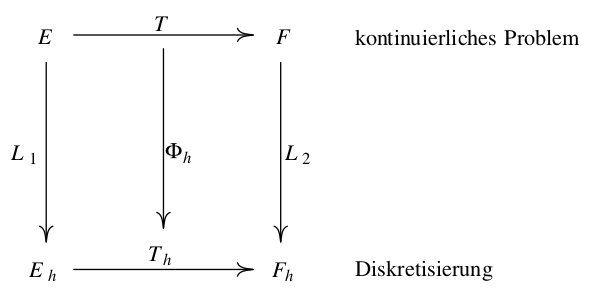
\includegraphics[width=0.45\textwidth]{abstraktkonsistenz.png} \\
	 	Abbildung aus \cite{brokate2016grundwissen} Seite 392
	 \end{figure}
	 Das diskretisierte Problem $ T_h \rho_h = 0  $ heißt genau dann konsistent, wenn für eine analytische Lösung $ \rho^{\star} \in E $ gilt, dass $ \lim\limits_{h \to 0}\lVert \Phi_h(T)L_1\rho^{\star} - L_2T\rho^{\star} \rVert_{F_h} = 0 $.
	 Betrachten wir zunächst in einem Zwischenschritt die Semidiskretisierung (5.3).
	 Die gewählte Herleitung dieser Formulierung soll dabei nahelegen, dass für eine exakte (und glatte) Lösung $ \rho $ die Konsistenz für die Semidiskretisierung erfüllt ist. In oben eingeführter Notation gilt also gerade $ B_h(\rho^{\star},\phi) $ für alle Testfunktionen $ \phi $. Auch wenn es sich bei $ Q_h $ um einen nicht konformen Ansatzraum handelt, ist der Herleitung der Semidiskretisierung dennoch zu entnehmen, dass auch $ B_h(\rho^{\star},\phi_h) $ für alle $ \phi_h \in Q_h $ gilt $(\star)$.  Wichtig ist dabei unter anderem auch die Wahl der numerischen Flussfunktion, der upwind flux erhält aber gerade gewünschten Eigenschaften. 
	 Mehr dazu findet sich in \cite{Har08b}.
	 Für die Zeitdiskretisierung in Form der impliziten Mittelpunktsregel gilt als einstufige Gauß-Quadratur $ \lVert \Phi_h(T)L_1\rho^{\star} - L_2T\rho^{\star} \rVert_{F_h} = O(h^2)$, womit sie insbesondere konsistent ist. \\
	 Daher gilt so für das kombinierte Verfahren, dass eine klassische Lösung $ \rho^{\star} $ somit auch die Volldiskretisierung in obigem Sinne erfüllt. 
\subsubsection{Galerkin Orthogonalität}
Eine direkte Folgerung aus der Konsistenz und $ (\star) $ stellt die Galerkin Orthogonalität dar. Für eine Lösung der Semidiskretisierung $ \rho_h $ und eine analytische Lösung im klassischen Sinne $ \rho^{\star} $ gilt dann nämlich:
\[
 B_h(\rho^{\star}-\rho_h,\phi_h = 0) \quad \forall \phi_h \in \mathcal{Q}_h
\]
\subsubsection{Stabilität und Konvergenz}
Die Stabilität ist bei der numerischen Lösung der Transportgleichung einer der wesentlichen Gründe, weswegen wir das Discontinuous Galerkin Verfahren einem Standard-Finite-Elemente-Ansatz vorziehen. Es zeigt sich nämlich, dass ein normales Finite Elemente Verfahren, wie wir es zuvor bei der Lösung des Potentialströmungsproblems genutzt haben, beim Transportproblem instabil ist. Grund dafür ist, dass $ \lVert q \cdot \nabla \rho_h \rVert $ beliebig groß werden kann. Für die DG-Diskretisierung mit upwind flux kann hingegen gezeigt werden, dass die Lösung des Transportproblems stabil ist. Auf eine theoretische Stabilitätsanalyse möchten wir aber an dieser Stelle verzichten und verweisen z.B. auf \cite{Har08b}.
Ebenso wollen wir bezüglich der Konvergenz des Verfahrens auf entsprechende Literatur verweisen. Wir werden später Konvergenzannahmen stellen und diese in entsprechenden Experimenten verifizieren. In der Literatur finden sich aber auch theoretische Konvergenzbeweise, meist unter Verwendung vielfältiger funktionalanalytischer Grundlagen und unter gewissen Regularitätsvoraussetzungen an die bestimmte Lösung. Die theoretische Betrachtung von Discontinuous Galerkinverfahren ist bereits Gegenstand vielfältiger wissenschaftlicher Arbeiten, aber zugleich ein breites Feld, welches noch lange nicht vollständig erforscht ist. \\
%Im nächsten Abschnitt sollen nun schließlich die Überlegungen der letzten Abschnitte gebündelt werden und wir wollen die Multilevel Monte Carlo Methode bei der speziellen Anwendung auf das Transportproblem betrachten.







%%%%%%%%%%%%%%%%%%%%%%%%%%%%%%%%%
\newpage  % neuer Abschnitt auf neue Seite, kann auch entfallen
%%%%%%%%%%%%%%%%%%%%%%%%%%%%%%%%%
\section{Anwendung der Multilevel Monte Carlo Methode auf das Transportproblem}
\label{MLMCTP}
% !TeX root = bachelorarbeit.tex
Nachdem wir in Abschnitt 2 an einige Grundlagen erinnert, in Abschnitt 3 und 4 sowohl die Monte Carlo Methode, als auch die Multilevel Monte Carlo Methode eingeführt und in Abschnitt 5 das Transportproblem, sowie das Potentialströmungsproblem inklusive numerischer Verfahren, welche zur Lösung dergleichen genutzt werden können, erklärt haben, soll nun dieser Abschnitt dazu dienen, die bisherigen Ergebnisse zu bündeln und die Anwendung der Multilevel Monte Carlo Methode auf partielle Differentialgleichungen am Beispiel des Transportproblem nahe zu legen. Dabei nimmt dieser Abschnitt einen zentralen Platz in dieser Thesis ein, weswegen wir noch einmal darlegen wollen, was genau unser Ziel ist und wie wir die uns an dieser Stelle zu Verfügung stehenden Mittel einsetzen, um das Gewünschte zu erreichen. Sei hierzu $ \mathbb{T} = (0,T] $ für ein $ T>0 $.
\begin{align*}
&\text{Für ein stochastisches Flussvektorfeld } q: \Omega \times \overline{\mathcal{D}} \to \R^2 \text{, bestimme }\rho: \Omega \times \overline{\mathcal{D}} \times \mathbb{T} \to \R_{\geq 0}\\ 
&\text{ mit} \\
&\text{(pTP)} 
\begin{cases}
\begin{array}{rlll}
\partial_t \rho (\omega, x, t) + \dive(\rho(\omega,x,t)q(\omega,x)) &= 0 &\text{, für } (x,t) \in \mathcal{D} \times \mathbb{T} \\
\rho(\omega,x,t) &= \rho_{\text{in}}(x,t) &\text{, für } (x,t) \in \Gamma_{\text{in}} \times \mathbb{T} \\
\rho(\omega,x,0)  &= \rho_0(x) &\text{, für } x \in  \mathcal{D}
\end{array}
\end{cases} \\
&\text{ für die Anfangs- und Randwerte: } \\ 
&\begin{array}{llr}
g_N&: \Gamma_{\text{N}} \to \R \\
u_D&: \Gamma_{\text{D}} \to \R \\
\rho_{\text{in}}&: \Gamma_{\text{in}} \times \mathbb{T} \to \R_{\geq0} \\
\rho_0&: \mathcal{D} \to \R_{\geq0} \\
\end{array} \newline \\
&\text{ wobei } \partial \mathcal{D} = \Gamma_{\text{D}} \dot{\cup} \Gamma_{\text{N}}  \text{ und }  \Gamma_{\text{in}} \coloneqq  \{ z \in \partial \mathcal{D}: q(z)\cdot n(z) \leq 0 \} \subset  \partial \mathcal{D}
\end{align*}
Genauer sei $ Q(\omega) = J(\rho(\omega)) $ ein gegebenes Zielfunktional, dann ist es unser Ziel den Erwartungswert $ \mathbb{E}[Q(\omega)] $ möglichst genau zu bestimmen. Beispielsweise kann eine beliebige Norm von $ \rho(\omega) $ als Zielfunktional betrachtet werden.
Unser Modellproblem lautet also:

\begin{align}
\text{(MP)}
\begin{cases}
\label{Modellproblem}
&\text{Für ein stochastisches Flussvektorfeld } q: \Omega \times \overline{\mathcal{D}} \to \R^2 \\
&\text{und ein Zielfunktional } J \text{ , bestimme }  \mathbb{E}[J(\rho)]  \\
&\text{mit } \rho \text{ als Lösung von (pTP) inklusive Anfangs- und Randwerten}
\end{cases}
\end{align} 
Dabei erhalten wir das stochastische Flussvektorfeld $ q $, wie bereits in \ref{Probabilistisches Problem} erklärt selbst als Lösung des Potentialströmungsproblem.
Da wir an der numerischen Lösung partieller Differentialgleichungen interessiert sind und wir die im Allgemeinen unendlich dimensionale Lösung $ \rho $ durch eine endlich dimensionale Lösung $ \rho_{h,\Delta t} $ approximieren, betrachten wir $ Q_{h,\Delta t}(\omega) \coloneqq J(\rho_{h,\Delta t}(\omega )) $.
Wir nutzen dabei das in Abschnitt \ref{DG} behandelte Discontinuous Galerkin Verfahren zur Lösung des linearen Transportproblems. Außerdem werden wir im Folgenden eine uniforme Familie $ \{ \mathcal{T}_h \} $ von Zerlegungen von $ \mathcal{D} $ (vgl. Abschnitt \ref{num_pot} Definition \ref{FEMDISC}) als Diskretisierungsgitter für die Ortsdiskretisierung, sowie $ \mathbb{T}_{\Delta t} $ als Zerlegung von $ \mathbb{T} $ betrachten.
Insbesondere wählen wir später $ \Delta t $ in Abhängigkeit von $ h $, etwa $ \Delta t = c  h $ für ein $ c>0 $ und betrachten dann
$ Q_h(\omega) \coloneqq Q_{h,ch}(\omega) = J(\rho_h(\omega )) \coloneqq J(\rho_{h,ch}(\omega )) $.
An dieser Stelle sei betont, dass es sich in diesem Abschnitt bei $ \rho_h $ um eine volldiskrtisierte Approximation an $ \rho $ handelt und nicht die Semidiskretisierung aus Abschnitt \ref{DG} gemeint ist. Um die Notation im Folgenden zu erleichtern schreiben wir für $ a,b \in \R_{> 0} $ $ a \lesssim b $, falls $\frac{a}{b}$ gleichmäßig beschränkt und insbesondere unabhängig von den Parametern $ h $ und $ n $ ist.
\begin{Annahme}(Konvergenz im Erwartungswert des Zielfunktionals)\\
	\label{Annahme1}
	In obiger Situation gelte 
	\[ 
	\mathbb{E}[Q_h] \to \mathbb{E}[Q] \text{ für } h \to 0   
	\]
	Genauer existiere ein $ \alpha > 0 $, sodass
	\[
		\abs{\mathbb{E}[Q_h-Q]} \lesssim h^{\alpha}
	\]
	Wir nennen $ \alpha $ dann auch die Konvergenzrate von $ Q_h $.
\end{Annahme}


\subsection{Die Monte Carlo Methode}
Wie bereits im Kontext der numerischen Integration wollen wir die Monte Carlo Methode als Ausgangspunkt nutzen und anschließend bei der Betrachtung der Multilevel Monte Carlo Methode auch auf entscheidende Unterschiede zu und Vorteile gegenüber der Monte Carlo Methode eingehen.
Sowohl bei der Monte Carlo Methode, als auch bei der Multilevel Variante approximieren wir den Erwartungswert $ \mathbb{E}[Q_h] $ durch einen Schätzwert $ \widehat{Q}_h $. Um die Genauigkeit und die Kosten zu bemessen betrachten wir zum einen den sogenannten 'root mean square error' (RMSE) 
\begin{align}
	\label{RMSE}
	e( \widehat{Q}_h) \coloneqq \left(  \mathbb{E} \left[ (\widehat{Q}_h - \mathbb{E}[Q] )^2 \right] \right)^{\frac{1}{2}}
\end{align}
zum anderen die Anzahl an floating-point-Rechenoperationen $ C_{\epsilon}(\widehat{Q}_h) $, die benötigt werden um einen RMSE mit $ e( \widehat{Q}_h) \leq \epsilon $ zu erhalten.
Zu beachten ist hierbei, dass in dem RMSE einige Fehlerquellen gemeinsam betrachtet werden. So gehen sowohl der Finite Elemente Fehler des Potentialströmungsproblems (Approximation von $ q $ durch $ q_h $), der Discontinuous Galerkin Fehler des Transportproblems (Approximation von $ \rho $ durch $ \rho_h $), der Approximationsfehler der Approximation von $ Q $ durch $ Q_h $, als auch der statistische Fehler des Schätzers $\widehat{Q}_h$ in den RMSE mit ein. Insbesondere bedeutet also $ e( \widehat{Q}_h) \leq \epsilon $, dass alle oben genannten Fehlerquellen kleiner als $ \epsilon $ ausfallen. Betrachten wir also, wie bei der Monte Carlo Methode, welche wir gleich noch einmal kurz behandeln wollen, nur eine einzige Zerlegung $ \mathcal{T} $ der Familie $ \mathcal{T}_h $, so kann es sein, dass es gar nicht möglich ist den RMSE durch ein bestimmtes $ \epsilon $ zu beschränken, da einer der Approximationsfehler für das gewählte feste Level bereits alleine größer als $ \epsilon $ ist. Wir wollen diesen Sachverhalt im Hinterkopf behalten, denn auch bei der Multilevel Monte Carlo  Methode werden wir später initiale Level wählen, in der konkreten Anwendung geben wir aus praktischen Gründen sogar ein maximales Level an, welches wiederum unter Umständen einen RMSE $ e( \widehat{Q}_h) \leq \epsilon $ verhindern kann.\\
Bei der Standard Monte Carlo Methode schätzen wir $ \mathbb{E}[Q] $ durch den Mittelwert  $ n $ unabhängiger gleichverteilter Zufallssamples und erhalten so 
\begin{align}
	\label{MC-Schätzer}
	\widehat{Q}_{h,n}^{\text{MC}} \coloneqq \frac{1}{n} \sum_{i=1}^{n} Q_h(\omega_i) = \sum_{i=1}^{n} J(\rho_h(\omega_i))
\end{align}
Dabei modellieren wir das zufällige Flussvektorfeld $ q(\omega_i)  : \mathcal{D} \to \R^2 $, indem wir zunächst für $ \kappa(\omega_i) : \mathcal{D} \rightarrow (\R_{\text{sym}})^{d \times d} $ ein lognormal-verteiltes unabhängiges Zufallsfeld erzeugen und anschließend das Potentialströmungsproblem
\begin{align*}
\setlength\arraycolsep{1pt}
&\text{Für } \kappa(\omega_i) : \mathcal{D} \rightarrow (\R_{\text{sym}})^{d \times d} \text{, bestimme } u(\omega_i,\cdot):\overline{\mathcal{D}} \to \R \text{ und } q(\omega_i, \cdot): \overline{\mathcal{D}} \to \R^2 \text{ mit } \\
&\text{(PS)}
\begin{cases}
\begin{array}{rlll}
\dive (q(\omega_i,x)) &= 0  &\text{, für } x \in \mathcal{ D}\\  
q(\omega_i,x) &= - \kappa(\omega_i) \nabla u(\omega_i,x)  &\text{, für } x \in \mathcal{D}\\
-q(\omega_i,x) \cdot n &= g_N(x)  &\text{, für } x \in \Gamma_N \\
u(\omega_i,x) &= u_D(x)  &\text{, für } x \in \Gamma_D \\
\end{array}
\end{cases} \\
\end{align*}
lösen. Zur Erzeugung des lognormal-verteilten Zufallsfeldes können wir auf entsprechende Algorithmen zurückgreifen, in unserem Fall etwa dem sogenannten Circulant Embedding.
Der Algorithmus wurde 1997 erstmals in \cite{dietrich1997fast} vorgestellt und 
erzeugt Gauß'sche Zufallsfelder auf regulären Gittern und basiert auf der Fast Fourier Transformation, welche in der Literatur auch oft unter der Abkürzung FFT zu finden ist.
Dabei werden spezielle Strukturen der Kovarianzmatrix ausgenutzt. Anschließend kann das Gauß'sche Zufallsfeld über eine einfache Transformation in ein lognormal Feld überführt werden. Mehr zu Circulant Embedding findet sich z.B. in \cite{schmidt2014stochastic} Abschnitt 12.
Auch die grundsätzliche Idee Circulant Embedding für die Modellierung der Ausgangsdaten in stochastischen partiellen Differentialgleichungen zu nutzen ist keineswegs neu und findet sich z.B. in \cite{charrier2012strong} oder \cite{cliffe2011multilevel}.
Wir haben nun alle Mittel in der Hand um die Monte Carlo Methode angewandt auf das Transportproblem als Algorithmus zu formulieren. Dabei fassen wir die eben erklärte Erzeugung des zufälligen Vektorfeldes in der Funktion 'RndVecField' zusammen.
Außerdem gehen wir davon aus, dass bereits alle übrigen freien Parameter, sowie die Rand- und Anfangswerte fest gewählt sind.
\begin{algorithm}[H]
	\DontPrintSemicolon
	\SetAlgoLined
	%\KwResult{}
	\SetKwInOut{Input}{Input}\SetKwInOut{Output}{Output}
	\Input{$h,n$}
	\Output{$\widehat{Q}_{h,n}^{\text{MC}}$}
	\BlankLine
	Initialisiere: $ \Sigma =0, i=0 $\;
	\While{$i<n$}{
		Erzeuge ein Zufallssample: $ q(\omega_i,x)  \leftarrow $ RndVecField\;
		Löse das Transportproblem: $ \rho_{h}(\omega_i,x)  \leftarrow$ Löse mit Discontinuous Galerkin\;
		Berechne das zugehörige Zielfuinktional: $ Q_h(\omega_i) \leftarrow$ Berechne Zielfunktional\;
		Setze: $ \Sigma = \Sigma + Q_h(\omega_i) $, i = i+1\;
	}
	\BlankLine
	\KwResult{$\widehat{Q}_{h,n}^{\text{MC}} = \Sigma /n$}
	\caption{Monte Carlo Methode angewandt auf das Transportproblem}
\end{algorithm}\bigskip % add 12pt space in-between

Wir nehmen an dieser Stelle an, dass sich die Gesamtkosten an Rechenoperationen, welche für die Berechnung eines $ Q_h(\omega_i) $ benötigt werden, durch
 \[
 	C(Q_h(\omega_i))  \lesssim h^{- \gamma}
 \] beschränken lassen.
 Im Folgenden wollen uns überlegen, wie wir unter dieser Annahme die Kosten für $ C_{\epsilon} $ abschätzen können. Diese Überlegungen finden sich auch in \cite{cliffe2011multilevel}.
 Der 'mean square error' $ e(\widehat{Q}_{h,n}^{\text{MC}})^2 $, also das Quadrat des RMSE, lässt sich nämlich auch folgendermaßen betrachten:
 \begin{align}
 \label{badumts}
 	e(\widehat{Q}_{h,n}^{\text{MC}})^2 &= \mathbb{E} \left[ \left( \widehat{Q}_{h,n}^{\text{MC}} -  \mathbb{E}[\widehat{Q}_{h,n}^{\text{MC}}] + \mathbb{E}[\widehat{Q}_{h,n}^{\text{MC}}] - \mathbb{E}[Q] \right)^2 \right] \nonumber \\
 	&= \mathbb{E} \left[ ( \widehat{Q}_{h,n}^{\text{MC}} -    \mathbb{E}[\widehat{Q}_{h,n}^{\text{MC}}]])^2 \right] + \left( \mathbb{E}[\widehat{Q}_{h,n}^{\text{MC}}] - \mathbb{E}[Q] \right)^2 \nonumber \\
 	&= \mathbb{V}[\widehat{Q}_{h,n}^{\text{MC}}] + \left( \mathbb{E}[\widehat{Q}_{h,n}^{\text{MC}}] - \mathbb{E}[Q] \right)^2
 \end{align}
 Dabei nutzen wir, dass für zwei unabhängige Zufallsvariablen $ a $ und $ b $ mit Erwartungswert $ \mathbb{E}[a] = 0 = \mathbb{E}[b] $ stets $ \mathbb{E}[(a+b)^2] = \mathbb{E}[a^2]+\mathbb{E}[b^2] $ gilt.
 Da weiter $ \mathbb{E}[\widehat{Q}_{h,n}^{\text{MC}}] = \mathbb{E}[Q_h] $ und $ \mathbb{V}[\widehat{Q}_{h,n}^{\text{MC}}] = \frac{1}{n^2} n \mathbb{V}[Q_h] = \frac{1}{n}  \mathbb{V}[Q_h] $ gilt, erhalten wir so 
 \begin{align}
 \label{mseMC}
	 e(\widehat{Q}_{h,n}^{\text{MC}})^2 = \underbrace{\frac{1}{n}  \mathbb{V}[Q_h]}_{(1)} + \underbrace{(\mathbb{E}[Q_h - Q])^2}_{(2)} \ .
 \end{align}
 Dabei ist (1), wie wir eben bereits gesehen haben, die Varianz des Monte Carlo Schätzers und spiegelt daher den Schätzfehler wider. Unter der zusätzlichen Annahme, dass Erwartungswert und Varianz des Schätzers existieren, konvergiert dieser Fehler nach dem starken Gesetz großer Zahlen für $ n \to \infty $ gegen $ 0 $.
 (2) hingegen hängt als Quadrat über den Gesamtapproximationsfehler zwischen $ Q_h $
 und $ Q $ nur von der Diskretisierungsschrittweite $ h $ ab. Ist das verwendete Lösungsverfahren konvergent, so geht (2) gegen $ 0 $ für $ h \to 0 $.
 Wollen wir den RMSE also durch ein $ \epsilon > 0 $ beschränken, ist es hinreichend dafür zu sorgen, dass sowohl (1) also auch (2) kleiner als $ \frac{\epsilon^2}{2} $ ausfallen. Wir müssen also $ h $ klein genug und zugleich $ n $ groß genug wählen.
 Genauer kann dies, unter der Annahme, dass $ \mathbb{V}[Q_h] $ annäherend konstant ist und somit nicht von $ h $ abhängt, erreicht werden, indem wir $ n \gtrsim \epsilon^{-2} $ und $ h \lesssim \epsilon^{\frac{1}{\alpha}}  $ (vgl. Annahme \ref{Annahme1}).
 Da wir weiter angenommen hatten, dass $ C(Q_h(\omega_i))  \lesssim h^{- \gamma} $ gilt, erhalten wir 
 \[ 
 	C(\widehat{Q}_{h,n}^{\text{MC}}) \lesssim n h^{-\gamma}
 \]
 und somit Gesamtkosten für einen erwarteten Schätzfehler kleiner als $ \epsilon $ von
 \begin{align}
	 C_{\epsilon}(\widehat{Q}_{h,n}^{\text{MC}}) \lesssim \epsilon^{-2-\frac{\gamma}{\alpha}}
 \end{align}
 
\subsection{Die Multilevel Monte Carlo Methode}

Wie wir bereits in Abschnitt \ref{MLMC} dargelegt haben, ist die entscheidende Idee der Multilevel Monte Carlo Methode Zufallssamples auf mehreren verschiedenen Leveln $ \{ h_l : l = 0,\dots,L \} $ mit $ h_0 > h_1 > \cdots > h_L $ zu betrachten. Wir erinnern an dieser Stelle daran, dass wir für die Menge aller betrachtbaren Level $ \mathcal{H} = \{ h_0 , h_1 \coloneqq \frac{h_0}{2},h_2 \coloneqq \frac{h_1}{2} = \frac{h_0}{4}, \dots \} $ gefordert hatten, insbesondere war hier $0 \in \overline{\mathcal{H}}$. Theoretisch gesehen berechnet der Algorithmus, welchen wir an späterer Stelle noch formulieren wollen, für ein gegebenes $ \epsilon $ nur Samples auf den für diese Genauigkeit benötigten Leveln, einer endlichen Untermenge von $ \mathcal{H} $. Die Menge der tatsächlich betrachteten Samples $ \tilde{\mathcal{H}} = \{ h_l : l = 0,\dots,L \} \subset \mathcal{H} $ ist also stets endlich.
Wie bereits in \ref{MLMC} erhalten wir 
\[
\mathbb{E}[Q_{h_L}] = \mathbb{E}[Q_{h_0}] + \sum_ {l=0}^L \mathbb{E}[Q_{h_l}-Q_{h_{l-1}}]  
\]
Um uns an dieser Stelle die Notation zu vereinfachen führen wir an dieser Stelle für $ l=0,\dots,L $ die Zufallsvariable $ Y_l $ ein mit $ Y_0(\omega) \coloneqq Q_{h_0}(\omega) = J(\rho_{h_0}(\omega)) $ und $ Y_l \coloneqq Q_{h_l}(\omega) - Q_{h_{l-1}}(\omega) =  J(\rho_{h_l}(\omega)) - J(\rho_{h_{l-1}}(\omega))  $ für $ l=1,\dots,L $. Man beachte hierbei, dass wie bereits an früher Stelle erwähnt, beim Vergleich zweier verschiedener Level das gleiche Sample zugrunde gelegt wird. 
So folgt:
\[
	\mathbb{E}[Q_{h_L}] = \sum_{l=0}^L \mathbb{E}[Y_l]
\]
Dann ist der Multilevel Monte Carlo Schätzer gegeben durch die Summe der Monte Carlo Schätzer $ \widehat{Y}_{h,n_l}^{\text{MC}} $ für die einzelnen Erwartungswerte $ \mathbb{E}[Y_l] $:
\begin{align}
	\widehat{Q}_{\tilde{\mathcal{H}},\{ n_l \}_{l=0}^L }^{\text{MLMC}} = \sum_{l=0}^{L} \widehat{Y}_{l,n_l}^{\text{MC}} =  \frac{1}{n_0} \sum_{i_0=0}^{n_0} Q_{h_0}(\omega_{i_0}) + \sum_{l=1}^{L} \frac{1}{n_l} \sum_{i=1}^{n_l} \left( Q_{h_l}(\omega_{i_l}) - Q_{h_{l-1}}(\omega_{i_l})\right)
\end{align}
Da für jedes $ l \ $ $ \widehat{Y}_{l,n_l}^{\text{MC}} $ getrennt berechnet und somit jeder Erwartungswert $ \mathbb{E}[Y_l] $ unabhängig geschätzt wird, erhalten wir die Varianz des MLMC-Schätzers durch $\mathbb{V}[ \widehat{Q}_{\tilde{\mathcal{H}},\{ n_l \}_{l=0}^L }^{\text{MLMC}} ] = \sum_{l=0}^{L} \frac{1}{n_l} \mathbb{V}[Y_l]$. Wie in \ref{badumts} lässt sich dann der mean square error dann ausdrücken durch:
\begin{align}
e(\widehat{Q}_{\tilde{\mathcal{H}},\{ n_l \}_{l=0}^L }^{\text{MLMC}})^2 &= \mathbb{E}  \left[ (\widehat{Q}_{\tilde{\mathcal{H}},\{ n_l \}_{l=0}^L }^{\text{MLMC}}- \mathbb{E}[Q])^2 \right] \nonumber \\
&= \mathbb{E}  \left[ (\widehat{Q}_{\tilde{\mathcal{H}},\{ n_l \}_{l=0}^L }^{\text{MLMC}} - \mathbb{E}[\widehat{Q}_{\tilde{\mathcal{H}},\{ n_l \}_{l=0}^L }^{\text{MLMC}}]+\mathbb{E}[\widehat{Q}_{\tilde{\mathcal{H}},\{ n_l \}_{l=0}^L }^{\text{MLMC}}]- \mathbb{E}[Q])^2 \right] \nonumber \\
&= \mathbb{E} \left[  (\widehat{Q}_{\tilde{\mathcal{H}},\{ n_l \}_{l=0}^L }^{\text{MLMC}}-\mathbb{E}[\widehat{Q}_{\tilde{\mathcal{H}},\{ n_l \}_{l=0}^L }^{\text{MLMC}}])^2 \right] +  \left(  \mathbb{E}[\widehat{Q}_{\tilde{\mathcal{H}},\{ n_l \}_{l=0}^L }^{\text{MLMC}}] - \mathbb{E}[Q] \right)^2 \nonumber \\
&= \underbrace{\sum_{l=0}^L \frac{1}{n_l} \mathbb{V}[Y_l]}_{(1)} + \underbrace{\left( \mathbb{E}[Q_{h_L}-Q] \right)^2}_{(2)}
\end{align}
\begin{Bemerkung}Was lässt sich hieraus ablesen?
	\begin{itemize}
%		\item $ (2) $ stimmt mit $ (2) $ aus \ref{mseMC} überein. Insbesondere ist also wieder  $ h \lesssim \epsilon^{\frac{1}{\alpha}}  $ dafür hinreichend, dass der Diskretisierungs- und Lösungsfehler kleiner als $ \frac{\epsilon^2}{2} $  ausfällt.
%		\item Um also einen kleineren RMSE als $ \epsilon $ zu erhalten, muss auch $ (1) \leq  \frac{\epsilon^2}{2} $ gelten.
		\item Unter Annahme \ref{Annahme1} gilt $ \mathbb{V}[Y_l] = \mathbb{V}[Q_{h_l}-Q_{h_{l-1}}] \stackrel{l \to \infty}{\to} 0  $, das bedeutet für uns: Je größer $ l $ und damit je feiner die Gitterweite $ h_l $ ist, desto weniger Samples werden benötigt um $ \mathbb{E}[Y_l] $ zu schätzen.
		\item Das niedrigste betrachtete Level $ l = 0 $ kann unabhängig von $ \epsilon $ fest gewählt werden. So bleibt insbesondere die benötigte Anzahl an Rechenoperationen pro Sample auf dem niedrigsten Level konstant, auch wenn $ \epsilon \to 0 $ geht. Bei der tatsächlichen Anwendung muss allerdings $ h_0 $ so gewählt werden, dass zumindest ein Mindestmaß an Auflösung des Problems gegeben ist. Deswegen werden wir später beim Algorithmus die Level beginnend bei $ l_0 $ indizieren. Um in der Theorie aber die Notation so schlank wie möglich zu halten, haben wir uns bewusst dafür entschieden bei der Indizierung in der Theorie mit Level $ l=0 $ zu beginnen.
	\end{itemize}
\end{Bemerkung} 
Wir sind nun in der Lage folgendes zentrale Resultat aus \cite{cliffe2011multilevel} nachzuvollziehen:
\begin{Satz}$ \newline $
	\label{MLMCTheorem}
	Sei in obiger Situation $ \widehat{Y}_l \coloneqq  \widehat{Y}_{l,n_l}^{\text{MC}}$ der Monte Carlo Schätzer für $ Y_l  $ und $ C_l \coloneqq C(Y_l^{(i)}) $ die Anzahl der Rechenoperationen, welche für die Berechnung eines Samples von $ Y_l $ benötigt werden.
	Es seien $ \alpha,\beta,\gamma,c_1,c_2,c_3 > 0 $ Konstanten mit $ \alpha \geq \frac{1}{2} \min(\beta,\gamma) $ und
	\begin{enumerate}[label=(\alph*)]
		\item $\abs{\mathbb{E}[Q_{h_l}-Q]} \leq c_1 h^{\alpha}_l $ (vgl. Annahme \ref{Annahme1})
		\item $ \mathbb{V}[Y_l] = \mathbb{V}[Q_{h_l}-Q_{h_{l-1}}] \leq c_2 h_l^{\beta} $
		\item $ C_l \leq c_3 h_l^{-\gamma} $ \ .
	\end{enumerate}
	Dann existiert für jedes $ 0 < \epsilon < \frac{1}{e} $ ein $ L \in \N $ und ein zugehöriges $ h_L \in \mathcal{H} $, sodass für $ \tilde{\mathcal{H}} = \{ h_l \}_{l=0}^L \subset \mathcal{H } $ gelten:
	\[
	e(\widehat{Q}_{\tilde{\mathcal{H}},\{ n_l \}_{l=0}^L }^{\text{MLMC}})^2 = \mathbb{E} \left[ \left( \widehat{Q}_{\tilde{\mathcal{H}},\{ n_l \}_{l=0}^L }^{\text{MLMC}} - \mathbb{E}[Q] \right)^2 \right] < \epsilon^2 \ ,
	\]
	
	\[
	C_{\epsilon}(\widehat{Q}_{\tilde{\mathcal{H}},\{ n_l \}_{l=0}^L }^{\text{MLMC}}) \leq \tilde{c} 
	\begin{cases}
		\begin{array}{llr}
		&\epsilon^{-2} , &\text{falls } \beta > \gamma \\
		&\epsilon^{-2} \log(\epsilon)^2 , &\text{falls } \beta = \gamma\\
		&\epsilon^{-2-(\gamma-\beta)/\alpha} , &\text{falls } \beta < \gamma
		\end{array}
	\end{cases}
	\]
	Dabei darf $ \tilde{c}$  von $ c_1,c_2 $ und $ c_3 $ abhängen.
\end{Satz}
\begin{proof}
	Betrachten wir zunächst den Monte Carlo Schätzer $ \widehat{Y}_l $, so gilt nach den Rechenregeln für Erwartungswerte 
	\[
		\mathbb{E}[\widehat{Y}_l] = 
			\begin{cases}
				\begin{array}{llr}
						&\mathbb{E}[Q_{h_l}] , &l=0 \\
						&\mathbb{E}[Q_{h_l}-Q_{h_{l-1}}] , &l>0
				\end{array} \qquad (\star)
			\end{cases}
	\]
	Wir nehmen o.B.d.A an, dass $ h_0 = 1 $. Ist dies nicht der Fall, lassen sich die Konstanten $ c_1,c_2,c_3 $ und $ \tilde{c} $ entsprechend skalieren.
	Wir wählen nun $ L \coloneqq \lceil \alpha^{-1} \log_2 (\sqrt{2}c_1\epsilon^{-1}) \rceil < \alpha^{-1} \log_2 (\sqrt{2}c_1\epsilon^{-1}) +1 $ . 
	Dann gilt:
	\[
	2^{-\alpha} \frac{\epsilon}{\sqrt{2}} < c_1 2^{-\alpha  L} \leq \frac{\epsilon}{\sqrt{2}}  \qquad (\star \star)
	\]
	Mit $ (\star) $ und (a) gilt dann mit $ \tilde{\mathcal{H}} = \{0,\dots,L\} $
	\[
	\left( \mathbb{E}[\widehat{Q}_{\tilde{\mathcal{H}},\{ n_l \}_{l=0}^L }^{\text{MLMC}} - \mathbb{E}[Q]] \right)^2 = \left( \mathbb{E}[Q_{h_L}] - \mathbb{E}[Q] \right)^2  \leq c_1 h_L^{\alpha} = c_1 2^{-\alpha L} \leq \frac{1}{2} \epsilon^2 \ .
	\]
	Nach (6.8) ist
	\[ 
	 	e(\widehat{Q}_{\tilde{\mathcal{H}},\{ n_l \}_{l=0}^L }^{\text{MLMC}})^2 	= \underbrace{	\mathbb{V}[\widehat{Q}_{\tilde{\mathcal{H}},\{ n_l \}_{l=0}^L }^{\text{MLMC}}]}_{(1)} + \underbrace{\left( \mathbb{E}[Q_{h_L}-Q] \right)^2}_{(2)}	
	\].
	Für das gewählte $ L $ ist also bereits $ (2) \leq \frac{1}{2}\epsilon^2 $.
	Um also $ e(\widehat{Q}_{\tilde{\mathcal{H}},\{ n_l \}_{l=0}^L }^{\text{MLMC}})^2 < \epsilon^2 $ zu gewährleisten, müssen wir nachweisen, dass für entsprechend gewählte $ \{n_l\}_{l=0}^L $ auch (1) kleiner als $ \frac{1}{2}\epsilon^2 $ ausfällt.
	Wir nutzen dazu die linke Ungleichung aus $ (\star \star) $ und erhalten 
	\begin{align}
		\sum_{l=0}^{L} 2^{\gamma l} < \frac{2^{\gamma L}}{1 - 2^{- \gamma}} < \frac{2^{\gamma}(\sqrt{2}c_1)^{ \frac{\gamma }{\alpha} }}{1-2^{-\gamma}} \epsilon^{-\frac{\gamma}{\alpha}}
	\end{align}
	Wir führen nun eine Fallunterscheidung für das Verhältnis zwischen $ \beta $ und $ \gamma $ durch.
	\begin{enumerate}[label=(\roman*)]
		\item $ \beta = \gamma: $\\
		Wir setzen $ n_l = \lceil 2\epsilon^-2(L+1)c_2 2^{-\beta l} \rceil $ für $ l= 0,\dots,L $, dann gilt mit (b):
		\[
		\mathbb{V}[\widehat{Q}_{\tilde{\mathcal{H}},\{ n_l \}_{l=0}^L }^{\text{MLMC}}] = \sum_{l=0}^{L}\mathbb{V}[\widehat{Y}_l] \leq \sum_{l=0}^{L} c_2 n_l^{-1} 2^{- \beta l} \leq \frac{1}{2} \epsilon^2
		\] \.
		Somit gilt also $ e(\widehat{Q}_{\tilde{\mathcal{H}},\{ n_l \}_{l=0}^L }^{\text{MLMC}}) < \epsilon $.
		Für die Anzahl an insgesamt benötigten Rechenoperationen gilt dann mit (c):
		\begin{align*}
			C_{\epsilon}(\widehat{Q}_{\tilde{\mathcal{H}},\{ n_l \}_{l=0}^L }^{\text{MLMC}})  &\leq c_3 \sum_{l=0}^{L} n_l 2^{\gamma l} 
			\leq c_3 \left( 2 \epsilon^{-2}(L+1)^2 c_2 + \sum_{l=0}^{L} 2^{\gamma l} \right)
		\end{align*}
		Für $ \epsilon < e^{-1} < 1 $ ist $ 1 < \log \epsilon^{-1} $ und $ \epsilon^{- \frac{\gamma}{\alpha}} \leq \epsilon^{-2} \leq \epsilon^{-2}(\log \epsilon)^2$, da $ \alpha \geq \frac{1}{2} \gamma $.
		Nutzen wir nun $ L = \lceil \alpha^{-1} \log_2 (\sqrt{2}c_1\epsilon^{-1}) \rceil < \alpha^{-1} \log_2 (\sqrt{2}c_1\epsilon^{-1}) +1 $  erhalten wir 
		\[
			C_{\epsilon}(\widehat{Q}_{\tilde{\mathcal{H}},\{ n_l \}_{l=0}^L }^{\text{MLMC}}) \leq \tilde{c}_1 \epsilon^{-2} (\log \epsilon )^2 , \quad \text{ für ein }\tilde{c}_1>0
		\]
		\item $ \beta > \gamma: $\\
		Wir setzen $ n_l = \lceil 2\epsilon^{-2} c_2 (1-2^{-(\beta-\gamma)/2})^{-1} 2^{-(\beta-\gamma)l/2} \rceil $, dann ist
		\[
		\sum_{l=0}^{L} \mathbb{V}[\widehat{Y}_l] \leq \frac{1}{2}\epsilon^2\left( 1-2^{-(\beta - \gamma)/2} \right) \sum_{l=0}^{L} 2^{-(\beta - \gamma)l/2} < \frac{1}{2} \epsilon^2
		\].
		Mit $ n_l <  2\epsilon^{-2} c_2 (1-2^{-(\beta-\gamma)/2})^{-1} 2^{-(\beta-\gamma)l/2} +1 $ ist so 
		\[
			C_{\epsilon}(\widehat{Q}_{\tilde{\mathcal{H}},\{ n_l \}_{l=0}^L }^{\text{MLMC}}) \leq c_3 \left( 2\epsilon^{-2}c_2 \left( 1 - 2^{-(\beta-\gamma)/2}\right)^{-2} + \sum_{l=0}^{L}2^{\gamma l} \right) \ .
		\] 
		Wiederum folgt mit (6.9), $ \epsilon < e^{-1} <1 $ und $ \epsilon^{-\frac{\gamma}{\alpha}} \leq \epsilon^{-2} $, dass
		\[
			C_{\epsilon}(\widehat{Q}_{\tilde{\mathcal{H}},\{ n_l \}_{l=0}^L }^{\text{MLMC}}) \leq \tilde{c}_2 \epsilon^{-2}, \quad \text{  für ein }\tilde{c}_2>0
		\]
		\item $ \beta < \gamma $\\
		Wir setzen $ n_l =  \lceil  \epsilon^{-2} c_2 2^{(\gamma-\beta)L/2+1} \left( 1-2^{-(\gamma - \beta)/2} \right)^{-1} 2^{-(\beta+\gamma)l/2} \rceil $.
		Dann ist 
		\[
		\sum\limits_{l=0}^{L} \mathbb{V}[\widehat{Y}_l] < \epsilon^2 2^{-(\gamma-\beta)L/2 -1}\left( 1- 2^{-(\gamma-\beta)/2} \right) \sum_{l=0}^{L} 2^{(\gamma-\beta)l/2} < \frac{1}{2} \epsilon^2 . 
		\]
		Durch obige Wahl von $ n_l $ erhalten wir dann 
		\begin{align*}
			C_{\epsilon}(\widehat{Q}_{\tilde{\mathcal{H}},\{ n_l \}_{l=0}^L }^{\text{MLMC}}) &\leq c_3 \left( 2\epsilon^{-2} c_2 2^{(\gamma-\beta)L/2}(1-2^{-(\gamma-\beta)/2})^{-1} \sum_{l=0}^L 2^{(\gamma -\beta)l/2} + \sum_{l=0}^L 2^{\gamma l} \right) \\
			&\leq c_3 \left( 2\epsilon^{-2} c_2 2^{(\gamma-\beta)L}(1-2^{-(\gamma-\beta)/2})^{-2}  + \sum_{l=0}^L 2^{\gamma l} \right) \ .
		\end{align*}
		Nutzen wir nun ein letztes Mal $ (\star \star) $, so ist $ 2^{(\gamma-\beta)L} < \left( \sqrt{2}c_1 \right)^{\frac{\gamma-\beta}{\alpha}} 2^{\gamma-\beta} \epsilon^{-(\gamma-\beta)/\alpha} $ und mit $ \epsilon < e^{-1} < 1 $ gilt wegen $ \alpha \geq \frac{1}{2}\beta $ auch $ \epsilon^{-\frac{\gamma}{\alpha}} \leq \epsilon^{-2 -(\gamma - \beta)/\alpha} $.
		Mit (6.9) folgt dann 
		\[
		C_{\epsilon}(\widehat{Q}_{\tilde{\mathcal{H}},\{ n_l \}_{l=0}^L }^{\text{MLMC}}) \leq \tilde{c}_3 \epsilon^{-2-(\gamma-\beta)\alpha} , \quad \text{  für ein } \tilde{c}_3>0
		\]
	\end{enumerate}
	Mit $ \tilde{c} \coloneqq \max\{\tilde{c}_1,\tilde{c}_2,\tilde{c}_3\} $ folgt also die Behauptung.\\
\end{proof}
Wir haben also gezeigt, dass für ein gegebenes $ 0 < \epsilon < e^{-1} $ stets ein maximales Level $ L $ und zugehörige Anzahlen an Zufallssamples $ \{n_l\}_{l=0}^L $
existieren, sodass der Multilevel Monte Carlo Schätzer $ \widehat{Q}_{\tilde{\mathcal{H}},\{ n_l \}_{l=0}^L }^{\text{MLMC}} $ im RMSE höchstens $ \epsilon $ vom tatsächlichen Erwartungswert $ \mathbb{E}[Q] $ entfernt ist. Außerdem haben wir unter entsprechenden Voraussetzungen an $ \{n_l\}_{l=0}^L $ obere Schranken für die Anzahl der benötigten Rechenoperationen bewiesen.
Verglichen mit den Kosten für die Monte Carlo Methode erhalten wir so für alle zulässigen $ \alpha,\beta,\gamma $ einen theoretischen Kostenvorteil. 
Durch eine geschickte, konkrete Wahl von $ \{n_l\}_{l=0}^L $ lässt sich zudem für feste Kosten $ C(\widehat{Q}_{\tilde{\mathcal{H}},\{ n_l \}_{l=0}^L }^{\text{MLMC}} ) = \sum_{l=0}^{L} n_l C_l$ die Varianz des Schätzers minimieren.
Wie in \cite{giles_2015} näher erklärt kann hierfür 
\begin{align}
	\label{OptimalN}
	n_l = \left\lceil 2 \epsilon^{-2} \sqrt{\frac{\mathbb{V}[Y_l]}{C_l}} \left( \sum_{l=0}^{L}\sqrt{\mathbb{V}[Y_l]C_l} \right) \right\rceil
\end{align}
gewählt werden. Dabei ist $ \mathbb{V}[Y_l] $ die geschätzte Varianz und $ C_l $ die Anzahl der benötigten Rechenoperationen für ein einzelnes Sample auf Level $ l $.
Davon ausgehend können wir nun den Algorithmus formulieren:

 \begin{algorithm}[H]
 	\DontPrintSemicolon
 	\SetAlgoLined
 	%\KwResult{}
 	\SetKwInOut{Input}{Input}\SetKwInOut{Output}{Output}
 	\Input{$ \epsilon > 0 $, $ l_0,L_0 \in \N $ und $ N_0 = \{ n_{l_0},\dots,n_{L_0} \}$}
 	\Output{$\widehat{Q}_{\tilde{\mathcal{H}},\{ n_l \}_{l=l_0}^L }^{\text{MLMC}} $}
 	\BlankLine
 	
 	Setze $ \tilde{\mathcal{H}} = \{ l_0,\dots,L_0 \} $ und die Anzahl der benötigten Samples $ \Delta N = \{ \Delta n_l \}_{l=l_0}^{L_0} = N_0$ und $ i = 0 $\;
 	\While{$\Delta n_l > 0$ für mindestens ein $ l \in \tilde{\mathcal{H}} $ }{
 		\For{alle $ l \in \tilde{\mathcal{H}} $ mit $\Delta n_l > 0$ }{
 			Berechne Zielfunktional und benötigte Kosten: $ Y_l,C_l \leftarrow $ MonteCarloEstimator$(h_l,\Delta n_l)$\;
 			Update $ C_l,\abs{\mathbb{E}[Y_l]},\mathbb{V}[Y_l] $ und setze $n_l = \Delta n_l, \Delta n_l=0$\;
 		}
 		Schätze die Exponenten $ \alpha,\beta,\gamma $ mit den Annahmen von Satz \ref{MLMCTheorem} \;
 		Schätze optimales $ N_i = \{ n_{l_i},\dots,n_{L_i} \} $ mit (\ref{OptimalN}) und berechne $\Delta N = N_i - N_{i-1}$\;
 		Teste auf schwache Konvergenz $ \abs{\mathbb{E}[Q_{h_{L_{i}}}-Q_{h_{L_{i}-1}}]} < (2^{\alpha}-1)\frac{\epsilon}{\sqrt{2}} $\;
 		\eIf{nicht konvergiert}{
 			Setze $\tilde{\mathcal{H}} = \{ l_0,\dots,L_i,L_{i+1} \coloneqq L_i+1 \} $\;
 			initialisiere $ \Delta n_{L_{i+1}} $ und setze $ \Delta N = \{\Delta n_l\}_{l \in \tilde{\mathcal{H}}} $ \;
 			i = i+1 \;
 			
 		} {
 		 $ \Delta N = \{0,\dots,0\}$\;
 		}
 	
 	}
 	\BlankLine
 	\KwResult{$\widehat{Q}_{\tilde{\mathcal{H}},\{ n_l \}_{l=l_0}^L }^{\text{MLMC}} $}
 	\caption{MLMC angewandt auf das Transportproblem}
 \end{algorithm}
\bigskip % add 12pt space in-between
Dabei überprüfen wir beim Test auf schwache Konvergenz ob $ \abs{\mathbb{E}[Q-Q_{h_{L_i}}]} < \frac{\epsilon}{\sqrt{2}}$ (vgl. (6.8)).
Unter der Annahme \ref{Annahme1} testen wir also ob
\[
	\abs{\mathbb{E}[Q_{h_{L_{i}}}-Q_{h_{L_{i}-1}}]} < (2^{\alpha}-1)\frac{\epsilon}{\sqrt{2}}
\]
Zu beachten ist, dass diese Version des Algorithmus, ebenso wie die in \cite{giles_2015} etwas allgemeinere Variante von heuristischer Natur ist. Es kann je nach Problemstellung nicht garantiert werden, dass mit diesem Verfahren stets ein RMSE kleiner $ \epsilon $ erreicht werden kann.
Satz \ref{MLMCTheorem} liefert zwar gerade die Garantie, dass es einen Multilevel Monte Carlo Schätzer gibt, welcher einen kleineren RMSE als $ \epsilon $ besitzt, für die genaue Konstruktion brauchen wir allerdings a-priori Kenntnisse über die Konstanten $ c_1 $ und $ c_2 $. Obiger Algorithmus verzichtet hingegen auf diese a-priori Kenntnisse und schätzt diese Konstanten on-the-fly.
Bei der tatsächlichen Implementierung, welche wir später verwenden werden, geben wir außerdem ein $ L_{\max} $ vor. Der Algorithmus bricht ab, wenn $ L_{\max} $ überschritten werden würde, und liefert dann kein Ergebnis zurück.
Dies liegt aber weniger an obigem Algorithmus, sondern vielmehr an der Erzeugung des zufälligen Vektorfeldes $ q(\omega_i,x) \leftarrow \text{RndVecField} $. Hierbei werden für die Permeabilität $ \kappa(\omega_i) $ log-normal verteilte Zufallsfelder mithilfe des Circulant-Embedding Algorithmus erzeugt. Um diese Erzeugung möglichst effizient zu gestalten, werden dafür nötige komplexe Eigenwertberechnungen zu Beginn vor der eigentlichen Multilevel Monte Carlo Methode für alle möglichen Level $ \widehat{\mathcal{H}} = \{ l_0,\dots,L_{\max}\}$ durchgeführt.
In zukünftigen Arbeiten könnte dies unter Umständen aber auch insofern verbessert werden, dass diese Berechnung ebenfalls in den MLMC Algorithmus integriert wird, aber ohne den Effizienzgewinn durch die einmalige Eigenwertberechnung für jedes Level aufzugeben.
 
 
 
%\begin{itemize}
%	\item Theorie Konvergenzannahmen
%	\item Resultate Giles + parrallelFEM Paper
%	\item Algorithmus
%\end{itemize}
%


%%%%%%%%%%%%%%%%%%%%%%%%%%%%%%%%%
\newpage  % neuer Abschnitt auf neue Seite, kann auch entfallen
%%%%%%%%%%%%%%%%%%%%%%%%%%%%%%%%%
\section{Experiment}
% !TeX root = bachelorarbeit.tex

\subsection{Modellproblem}

In diesem Abschnitt wollen wir anhand des linearen Transportproblems auch tatsächliche praktische Resultate der Multilevel Monte Carlo Methode beleuchten.
Wir setzen dazu
\begin{itemize}
	\item $ \mathcal{D} = (0,1)^2 \subset \R^2 $ (also insbesondere wie breits zuvor in der Theorie $ n=2 $)
	\item $ \mathbb{T} = [0,T] = [0,1] $ (vgl. Bemerkung \ref{wahlfunk})
	\item $ \rho_{\text{in}} \equiv 0 $
	\item $ \rho_0(x) = 
	\begin{cases*}
		\begin{array}{llll}
			&c & , &\text{für }x \in B \coloneqq [0.2,0.8] \times [0.7 ,0.8]  \\
			&c\exp \left(\frac{ \left| \frac{\text{dist}(x,B)}{0.15} \right| ^2}{\left|\frac{\text{dist}(x,B)}{0.15}\right|^2-1}\right) &, &\text{falls } x \not \in B \text{ und dist}(x,B) < 0.15 \\
			&0 &, & \text{sonst}
		\end{array}
	\end{cases*}$ \\
	Dabei sei $ c $ so gewählt, dass 
	\[
		\int_{\mathcal{D}} \rho_0(x) \dx = 1 \ ,
	\]
	wir skalieren also die zu Beginn im Rechengebiet enthaltene Masse auf $ 1 $.
\end{itemize} 
Die Anfangskonzentration $ \rho_0 $ entspricht also gerade einer rechteckigen Ansammlung mit Länge $ 0.6$ und Breite $ 0.1$ und Mittelpunkt $ (0.5,0.75) $, welcher in beide Richtungen auf einem $ 0.15$ breiten Streifen mit einer Exponentialfunktion in die Ebene geglättet wird. 
Wir stellen so für die Anfangsbedingungen unseres Modellproblems einen sehr hohen Grad an Regularität sicher. 
Visuell kann diese Anfangskonzentration folgendermaßen dargestellt werden:
\begin{figure}[H]
	\centering
	\captionabove{Anfangsbedingung $ \rho_0 $}
	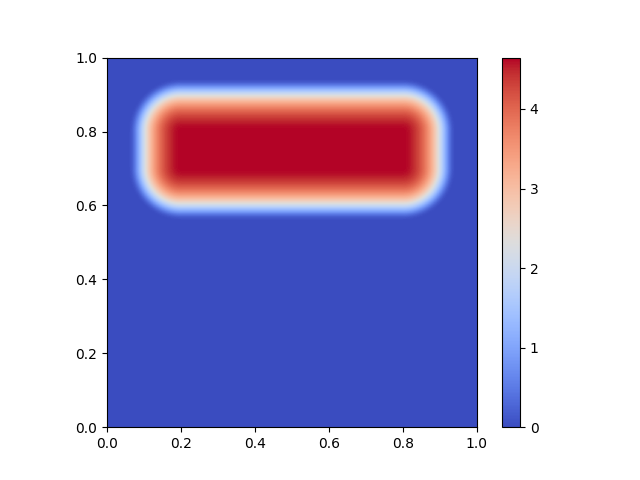
\includegraphics[width=0.65\textwidth]{plots/anfangsbedingung.png} 
\end{figure}
Der Maximalwert ist dabei so gewählt, dass die Gesamtmasse der Anfangsbedingung gerade den Wert $ 1 $ ergibt.\\
Uns interessiert nun folgende Fragestellung: \\
\textbf{Wie groß ist der erwartete Anteil der Masse, welcher nach Ablauf des betrachteten Zeitintervalls $ \mathbb{T} $ im Rechengebiet $ \mathcal{D} $ verbleibt?}\\

Wie bereits an früherer Stelle erklärt, berechnen wir hierzu ein stochastische Flussvektorfeld $ q : \Omega \times \overline{\mathcal{ D}} \to \R^2 $ als Lösung des zugehörigen Potentialströmungsproblems, wobei wir dabei den Permeabilitätstensor $ \kappa : \Omega \times \mathcal{D} \to \R_{\geq0} $ als lognormal verteiltes Zufallsfeld modellieren. Wir identifizieren dabei die Verteilung von $ \kappa $ mit der zugehörigen Kovarianzfunktion:
\[
 C(x,y) = \sigma^2 \exp(- \frac{\lVert x-y \rVert_2^s}{\lambda^s} ) .
\]
Dabei ist $ 0 < \sigma^2 < \infty $ die Varianz des zugrundeliegenden Gauß'schen Zufallsfeldes, durch $ \lambda = (\lambda_1,\lambda_2) \in \R^2 $ werden die Korrelationslängen in die verschiedenen Koordinatenrichtungen gegeben und $ s \in (1,2) $ ist ein Glättungsparameter. Wir wählen an dieser Stelle :
\begin{align*}
s &=  1.9\\
\lambda_1,\lambda_2 &= 0.15\\
\sigma &= 1.0
\end{align*}
Wir können auch das lognormal verteilte Zufallsfeld und das daraus resultierende stochastische Flussvektorfeld $ q $ exemplarisch für ein $ \omega \in \Omega $ grafisch darstellen. Bei der Visualisierung des Flussvektorfeldes nutzen wir dabei einen sogenannten 'Quiverplot'. Im Wesentlichen wird dabei FLussvektorfeld auf einem Gitter ausgewertet und die resultierenden Vektoren mithilfe eines Skalierungsparameters skaliert, damit die so eingezeichneten Vektoren eine dem Gitter angepasste Länge besitzen.

\begin{figure}[H]
	\centering
	\captionabove{Visualisierung der stochastischen Modellierung}
	\subfigure[lognormal verteiltes Zufallsfeld mit obigen Parametern]{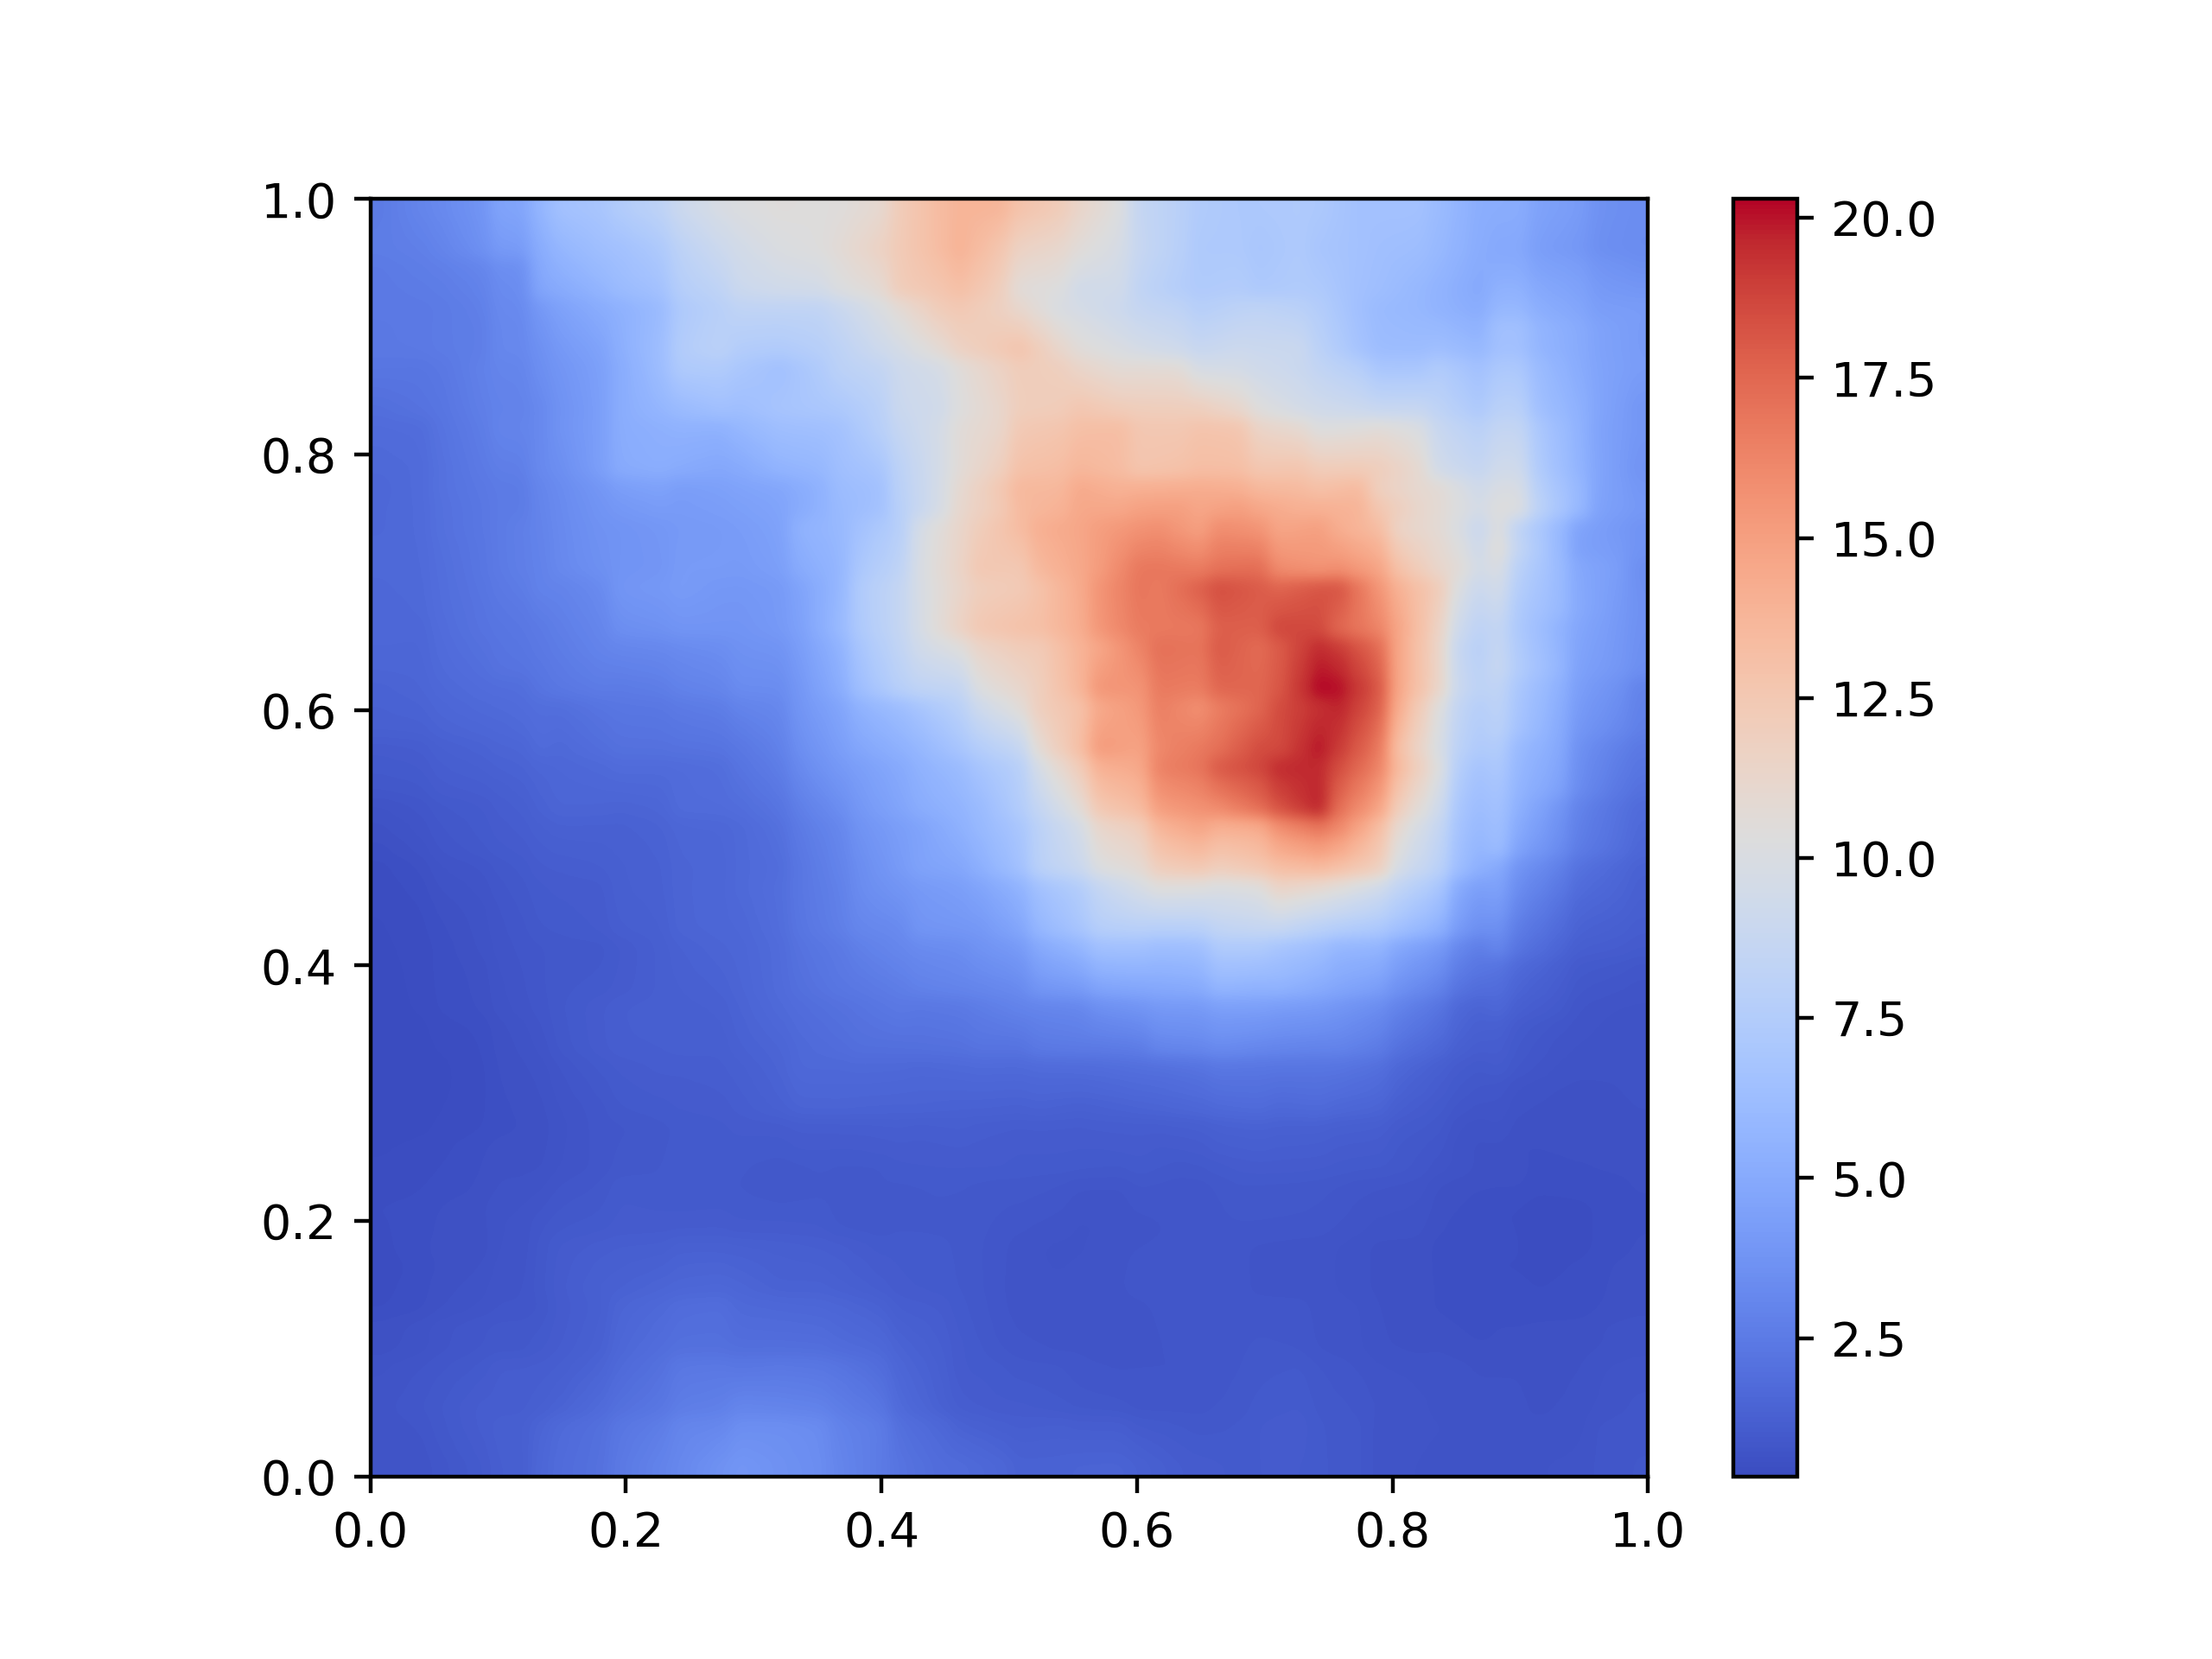
\includegraphics[width=0.49\textwidth]{plots/perm.png}}
	\subfigure[Zufallsfeld und zugehöriges  Flussvektorfeldes]{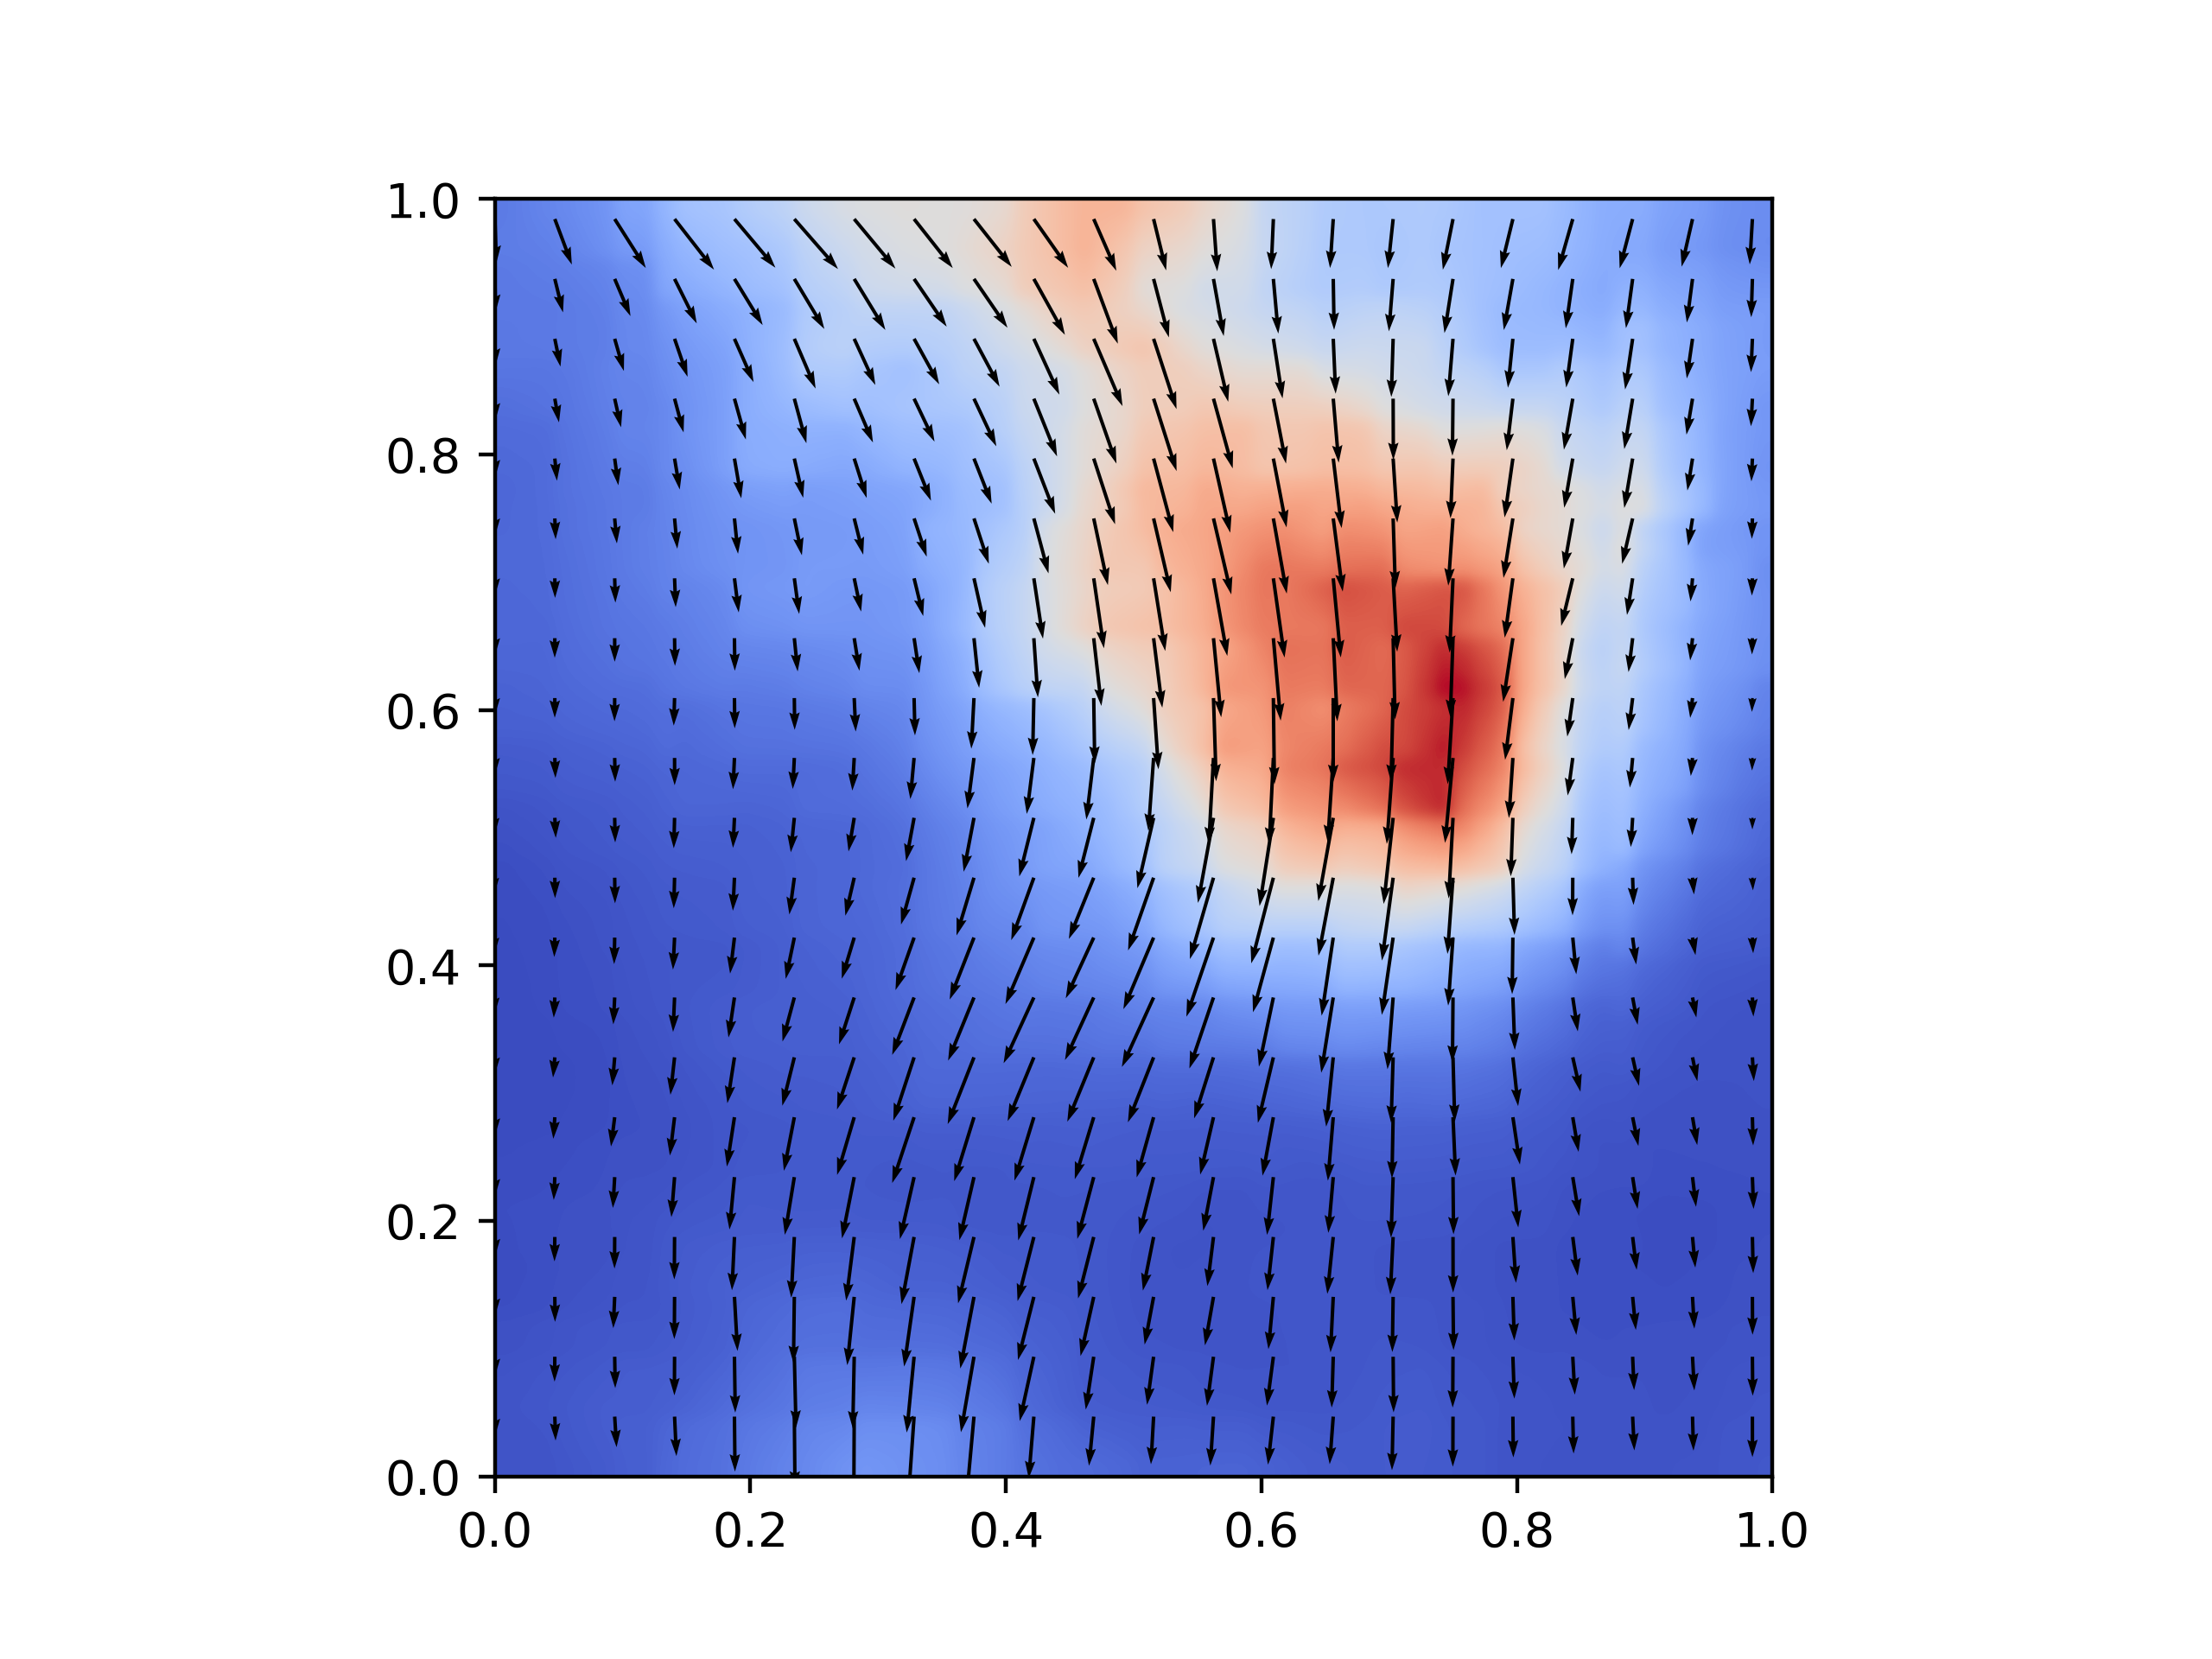
\includegraphics[width=0.49\textwidth]{plots/permquiv.png}}
	
\end{figure}

Weiter setzen wir
\begin{itemize}
	\item $\Gamma_{\text{D}} = \{ x = (x_1,x_2) \in \overline{\mathcal{D}} : x_2 = 0 \} $
	\item $ \Gamma_{\text{N}} = \partial \mathcal{D} \setminus \Gamma_{\text{D}} $
	\item $ g_N = \begin{cases}
						\begin{array}{llll}
						    &0 &, &\text{falls } x \in \{ x \in \Gamma_{\text{N}} : x_1 \in \{ 0,1 \}  \} \\
						    &1 &,& \text{sonst}
						\end{array}
				  \end{cases} $
	\item $ u_D \equiv 0 \text{ auf } \Gamma_{\text{D}} $
	
\end{itemize}

Als Zerlegung von $ \mathcal{D} $ wählen wir gleichartige Quadrate. Um auf dem geringsten Level ein Mindestmaß an Auflösung zu gewährleisten, wählen wir auf Level $ l_0 $ eine Zerlegung in $ 256 = 16^2 $ Quadrate. Dies entspricht einer Ortsdiskretisierungsschrittweite von $ h_0 = \frac{1}{16} = 0.0625 $. Wie bereits im Theorieteil angemerkt, wählen wir von $ h_0 $ ausgehend die uniforme Familie von Zerlegungen $ \{\mathcal{T}_h \}_{h \in \mathcal{H}} $ mit $ \mathcal{H} = \{ h_0 , h_1 \coloneqq \frac{h_0}{2},h_2 \coloneqq \frac{h_1}{2} = \frac{h_0}{4}, \dots \} $. Auf Level $ l_1 $ betrachten wir also $ 1024 = 32^2 $ und auf Level $ l_k $ dementsprechend $ 2^{2(k+4)} $ Quadrate. 
In M++ entspricht Level $ l_0 $ bei der gewählten Diskretisierung 'UnitSquare' gerade Level $ 4 $. Die Zerlegungen auf $ l_0 = 4, l_1 = 5 $ und $ l_2 = 6 $ lassen sich folgendermaßen darstellen:
\begin{figure}[H]
	\centering
	\captionabove{Zerlegung des Gebietes $ \mathcal{D} $ in Finite Elemente}
	\subfigure[$l_0 = 4$ (256 Zellen)]{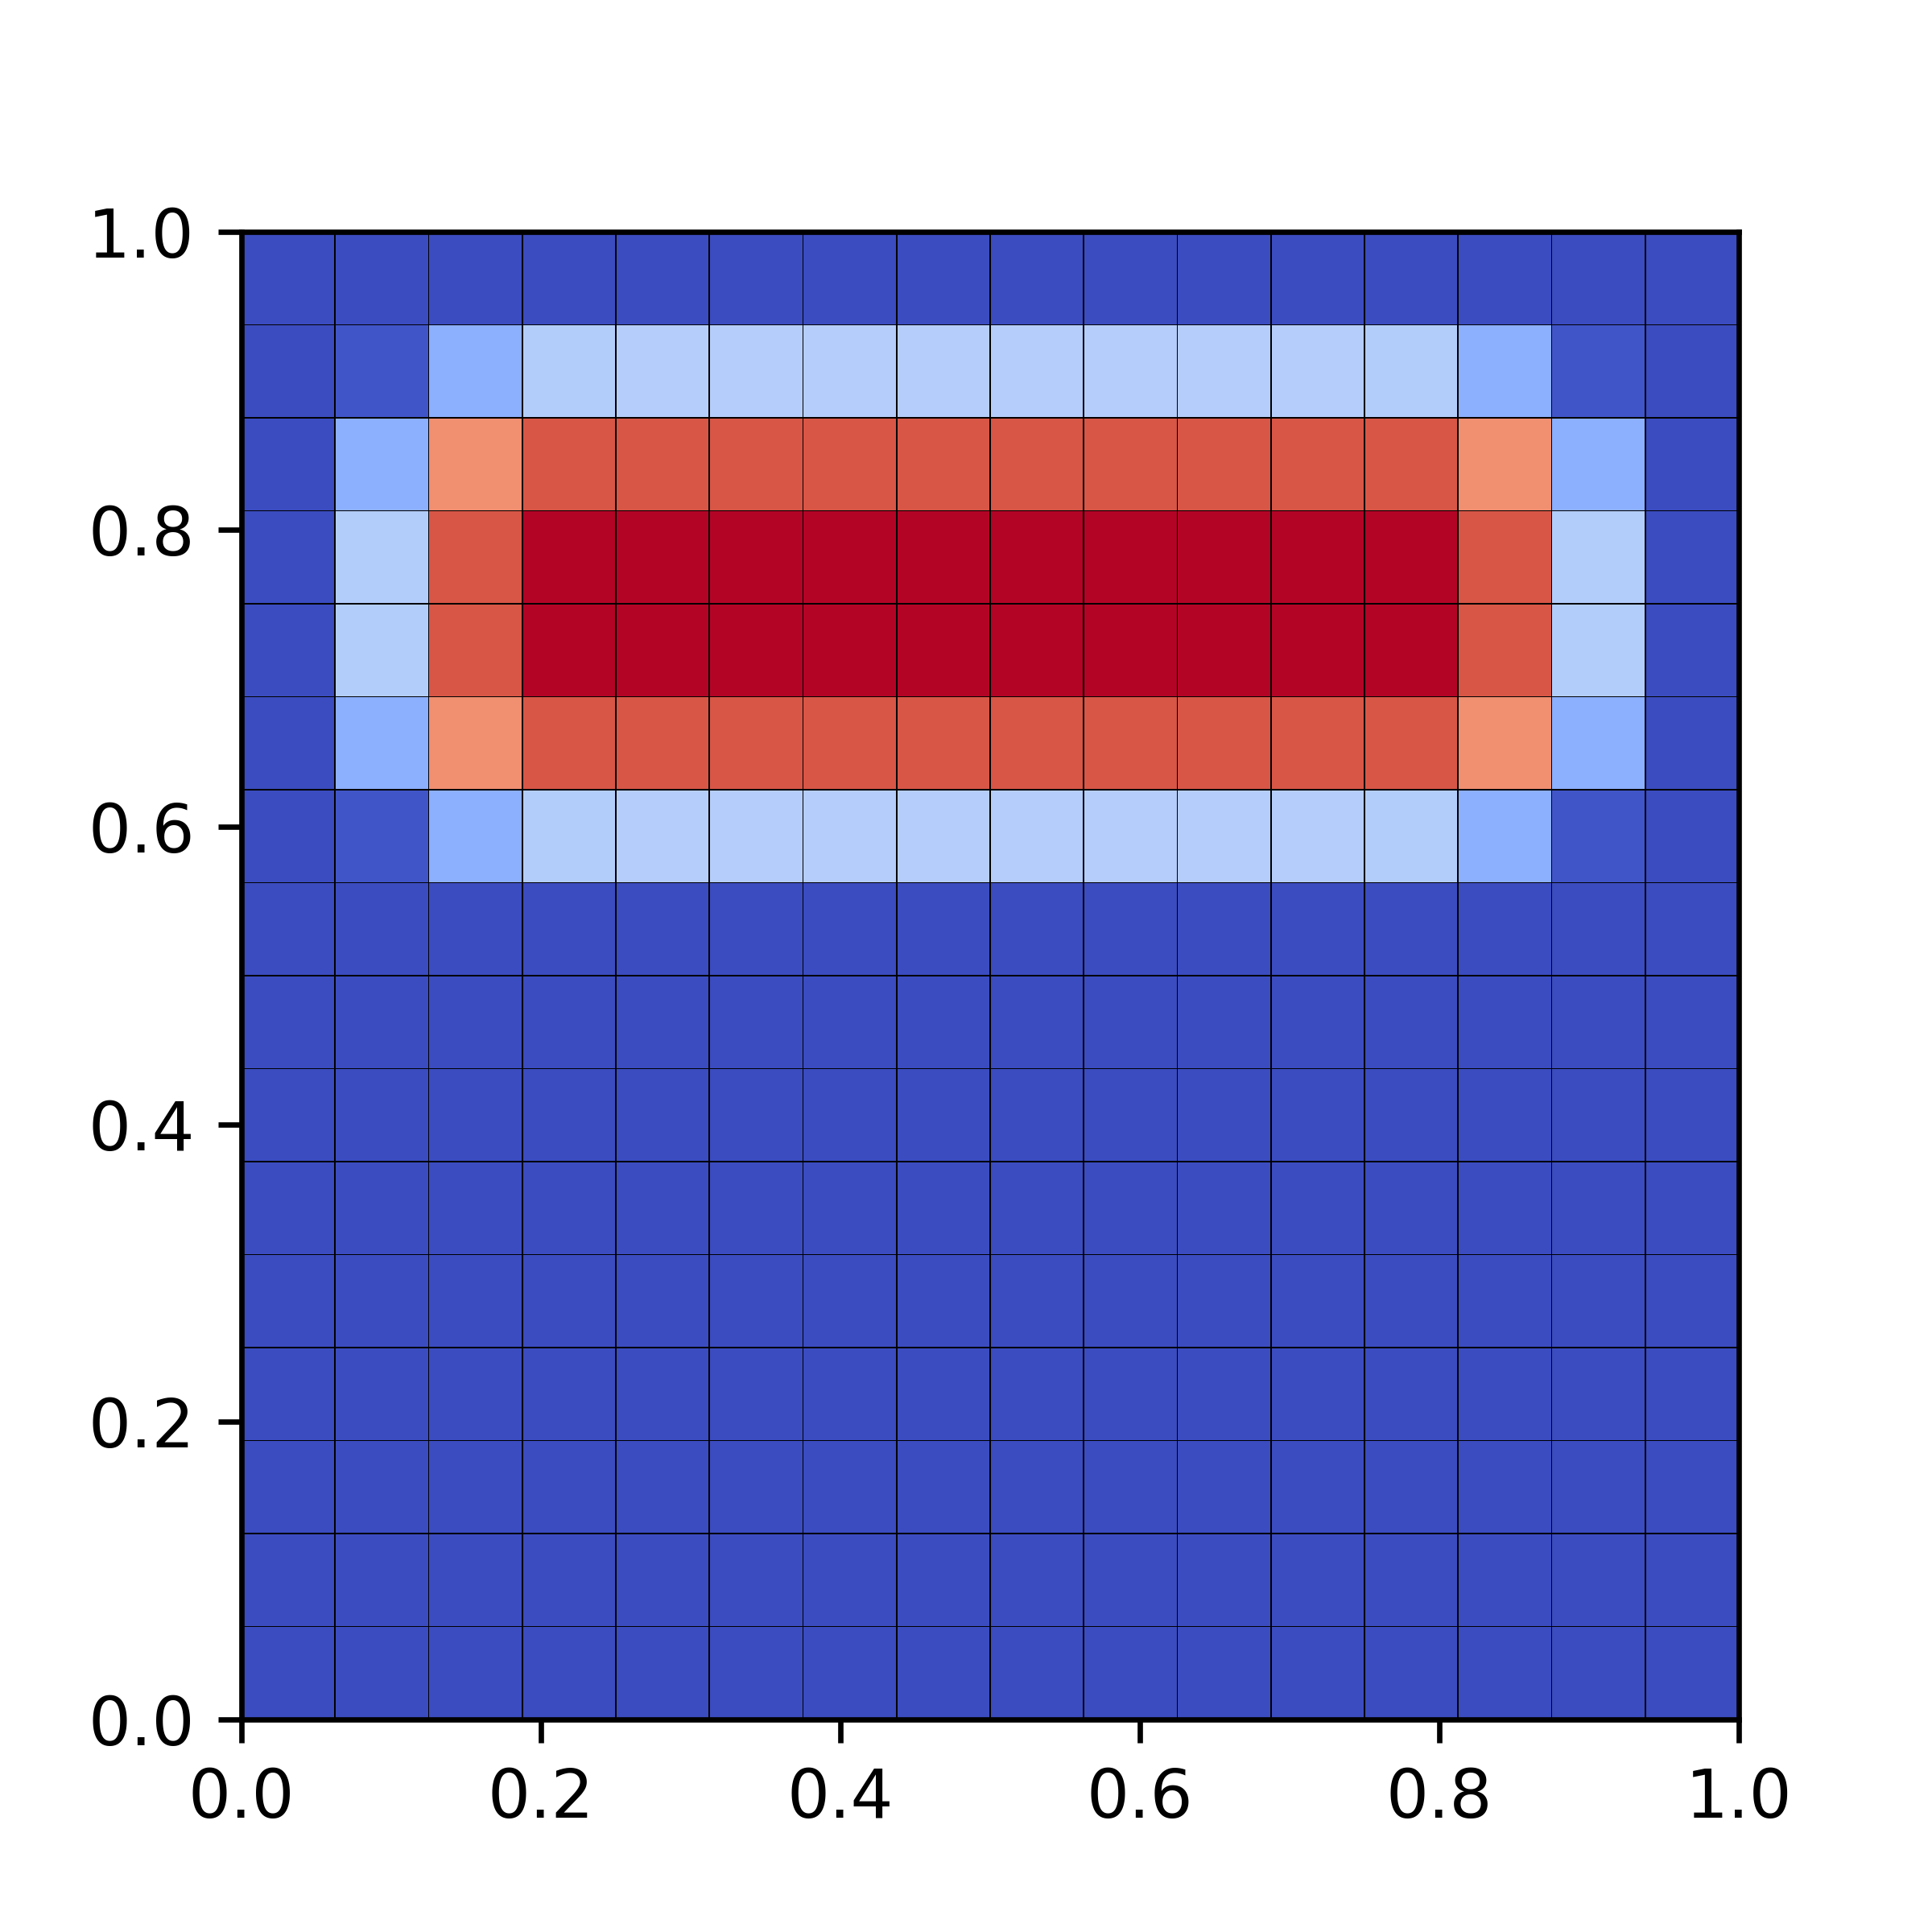
\includegraphics[width=0.31\textwidth]{plots/mesh4.png}}
	\subfigure[$l_1 = 5$ (1024 Zellen)]{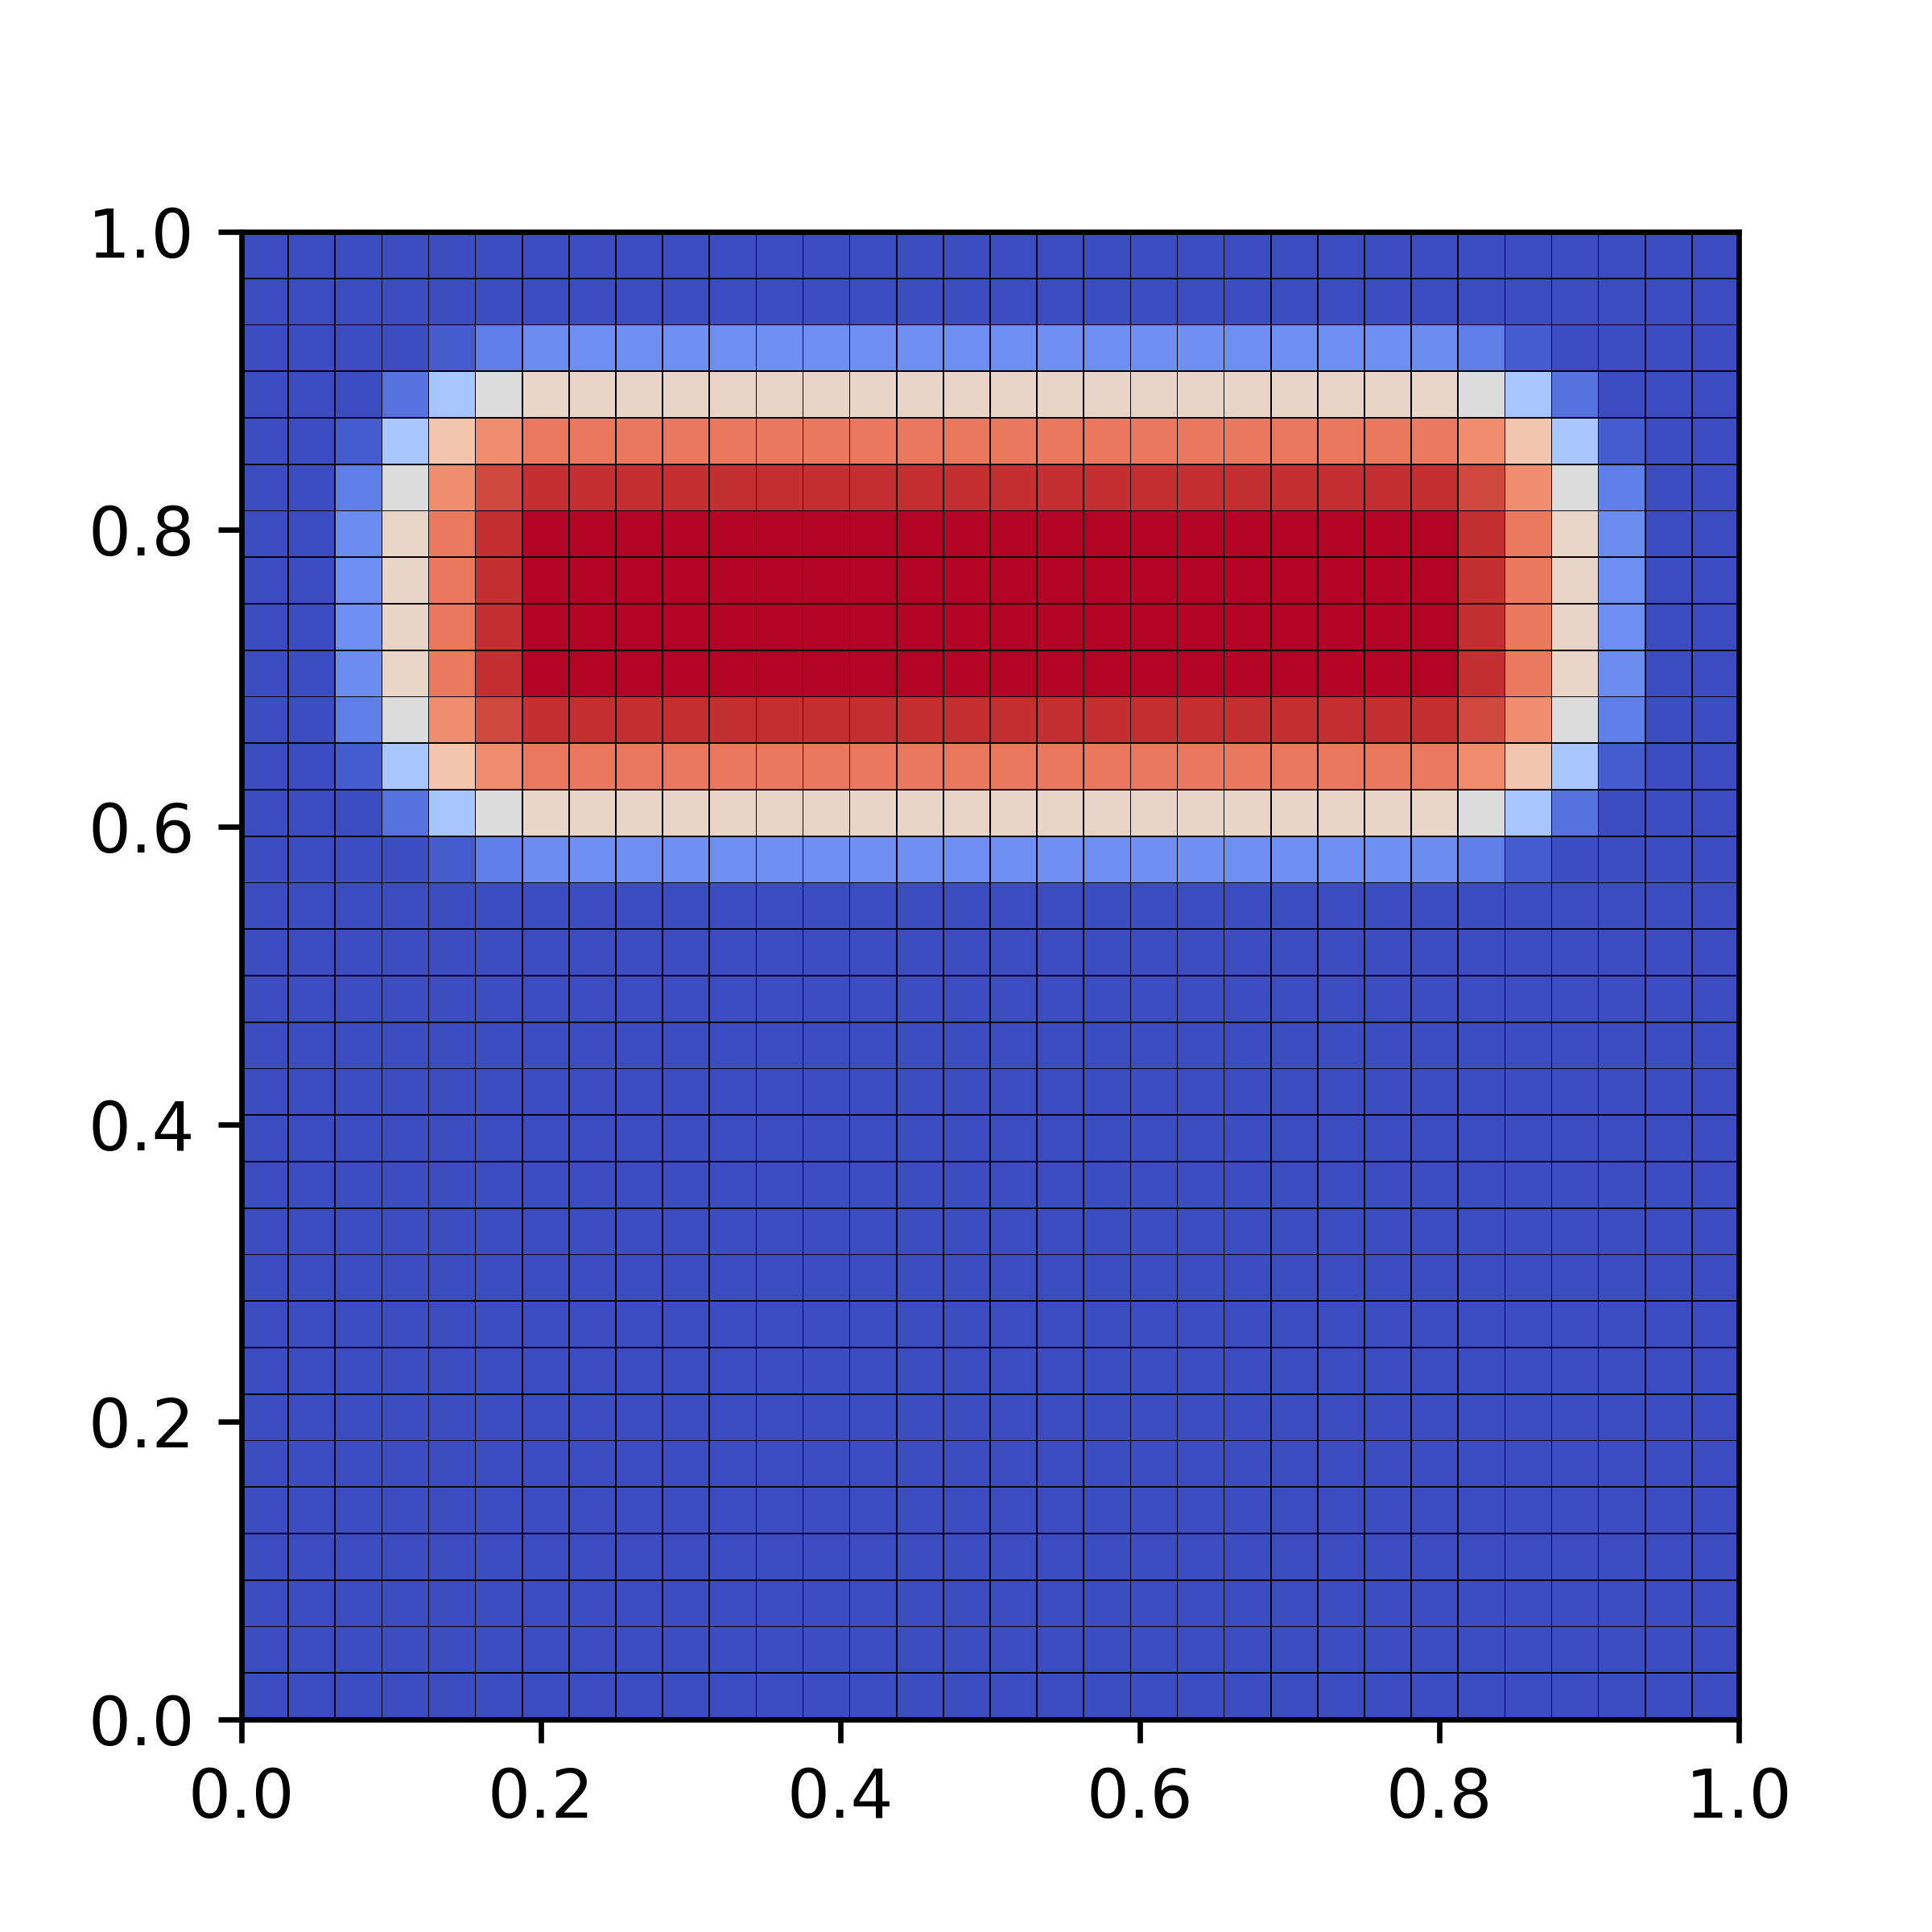
\includegraphics[width=0.31\textwidth]{plots/mesh5.png}}
	\subfigure[$l_2 = 6$ (4096 Zellen)]{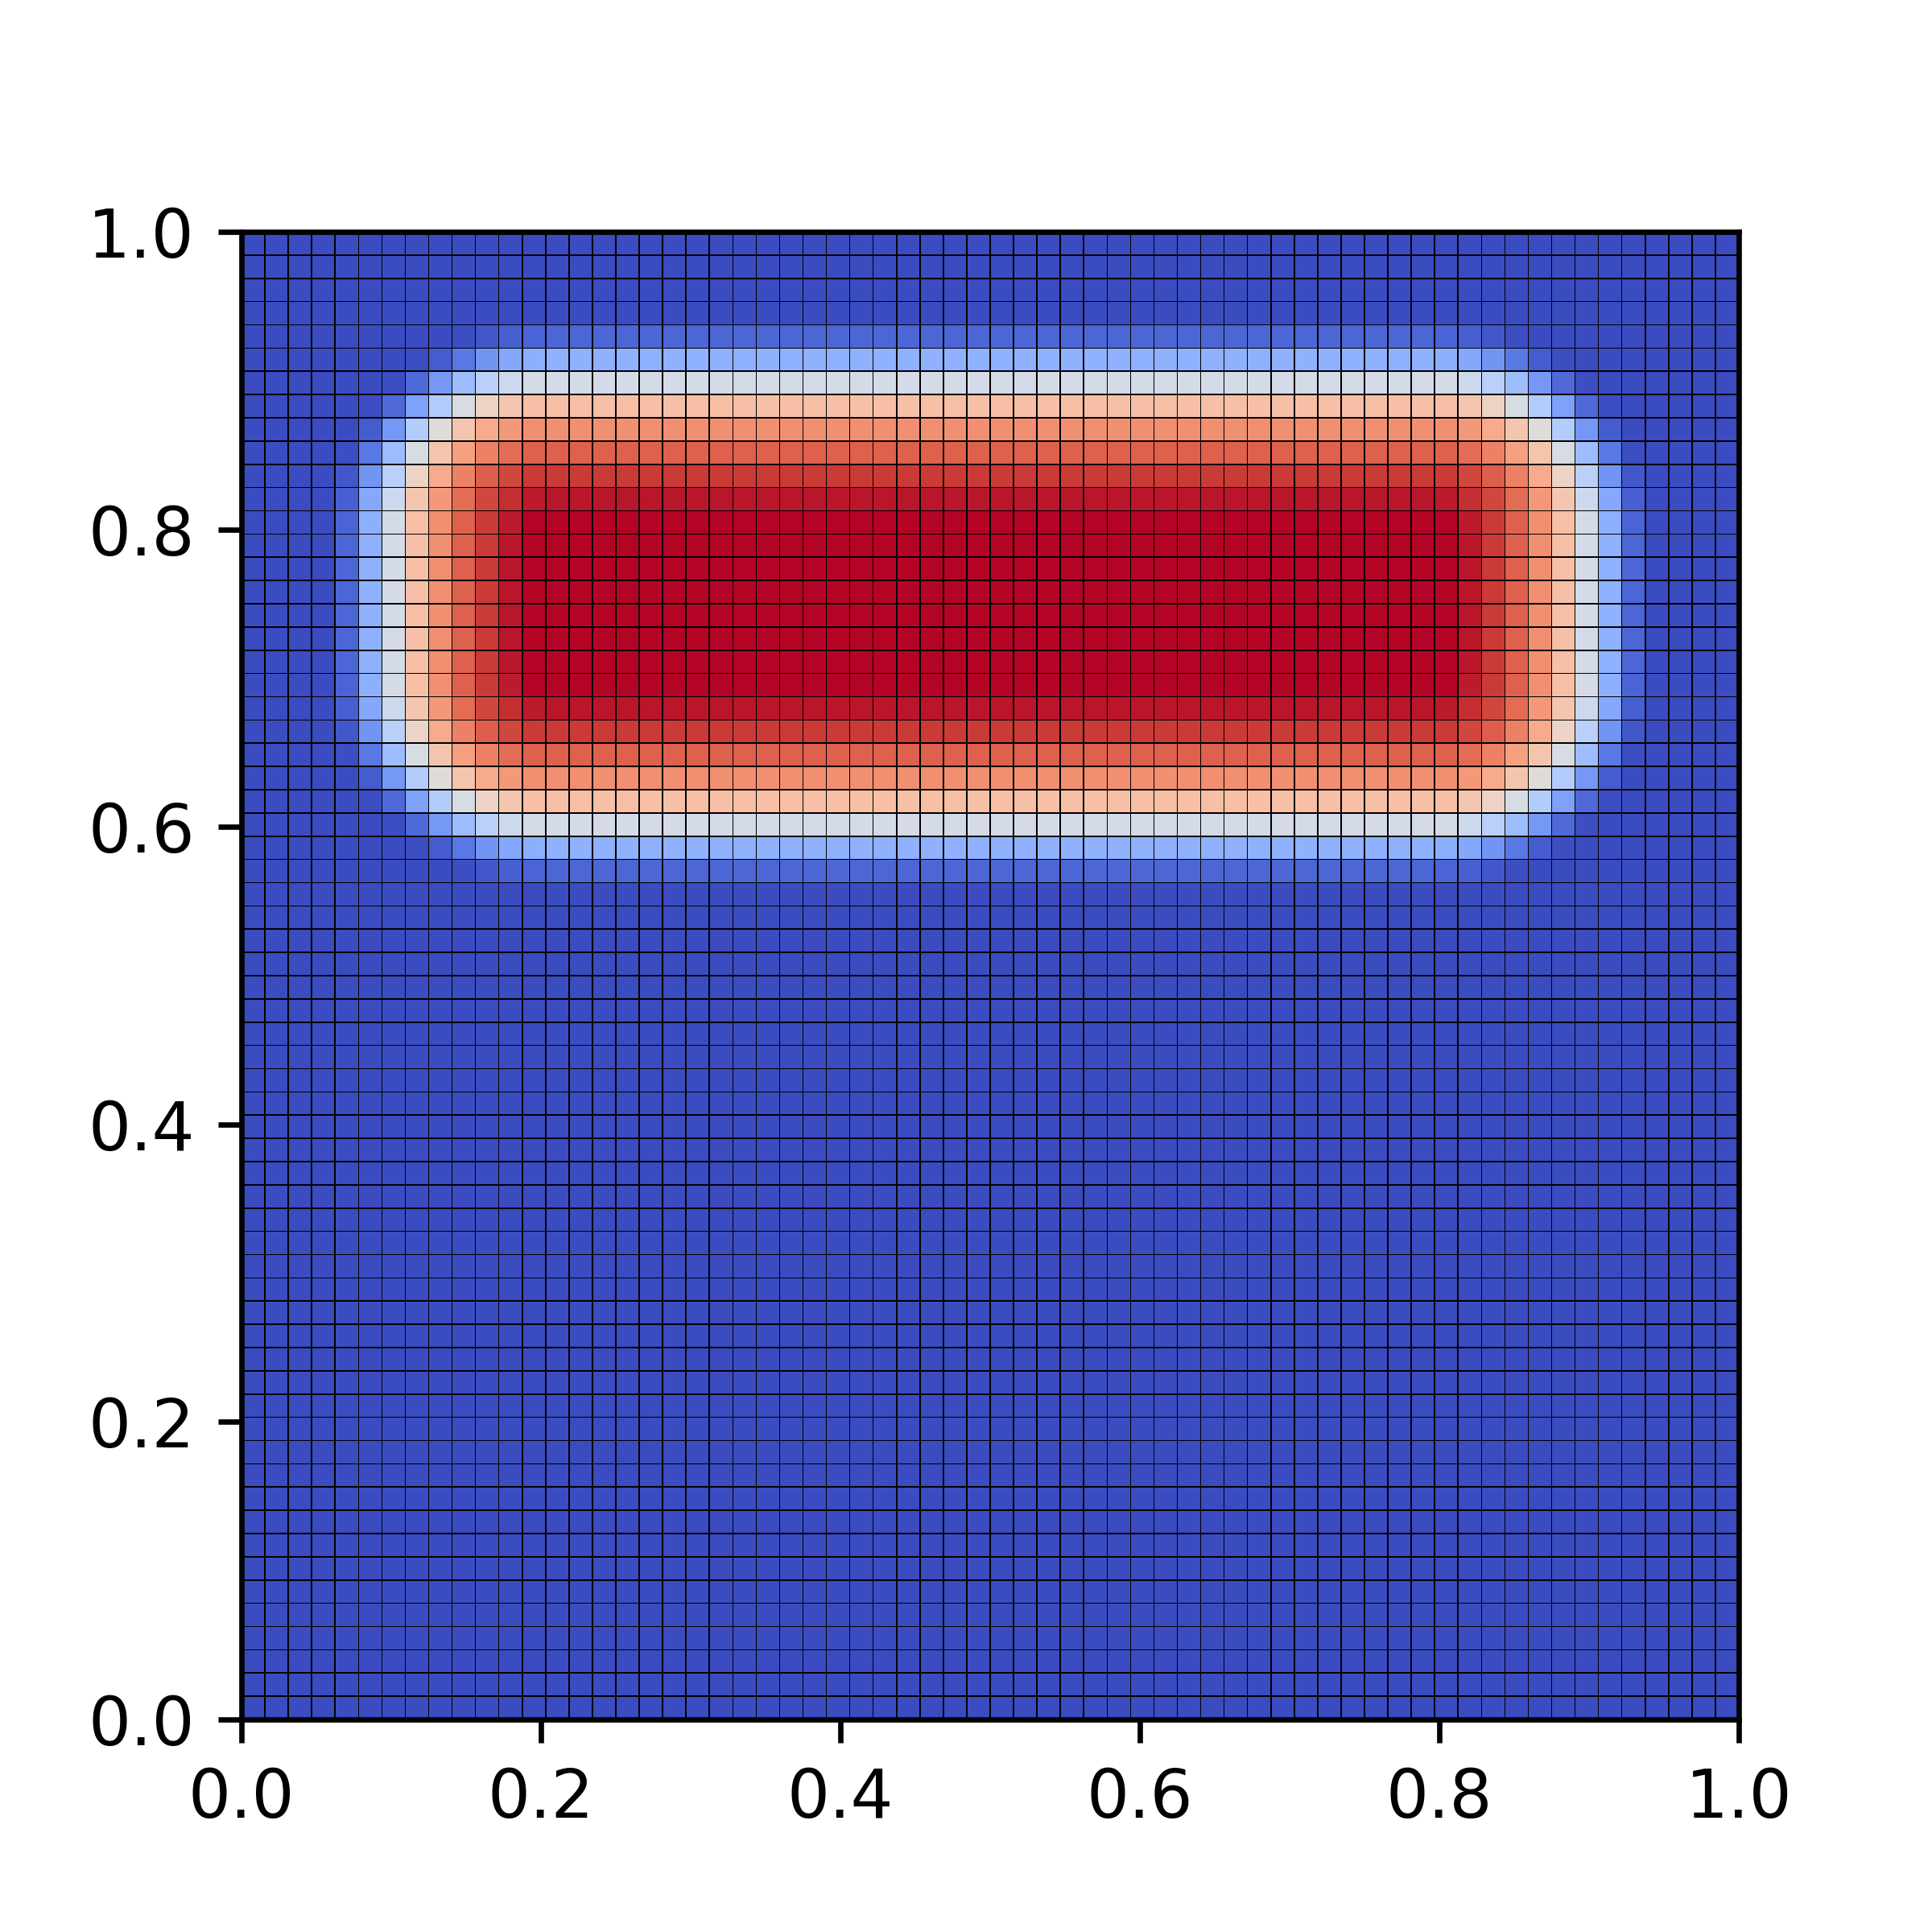
\includegraphics[width=0.31\textwidth]{plots/mesh6.png}}
\end{figure}
Die Schrittweite für die Diskretisierung in der Zeit setzen wir auf $ \Delta t = \frac{h}{8} $. Diese Wahl ist besonders hinsichtlich der Stabilität des Verfahrens wichtig. Bei zu kleinen Zeitschrittweiten treten Oszillationen in der Lösung auf. Obige Wahl hat sich für unser Problem als hinreichend erwiesen.
Entsprechend unserer Fragestellung können wir nun das betrachtete Zielfunktional formulieren:
\[
Q(\omega) = J(\rho(\omega)) \coloneqq \int_{\mathcal{D}} \rho(\omega,x,T) \dx = \int_{\mathcal{D}} \rho(\omega,x,1) \dx
\]
Wir suchen gemäß unserer Fragestellung also gerade nach $ \mathbb{E}[Q] $.
\begin{Bemerkung2}\label{wahlfunk}
	Die Wahl $ T=1 $ ist an dieser Stelle gerade so getroffen, dass das der Fragestellung entsprechende Zielfunktional in gewisser Weise interessant ist. 
	Genauer ist $ T $ so gewählt, dass die im Algorithmus auftretende Varianz $ \mathbb{V}[Y_l] $ 'groß' ausfällt. Ist $ T $ nämlich zu groß gewählt, befindet sich für fast alle $ \omega \in \Omega $ kaum noch Masse im Gebiet und die erwartete Endmasse ist $ \mathbb{E}[Q] = 0 $, während für sehr kleine $ T $ Masse zum Zeitpunkt $ T $ für fast alle $ \omega \in \Omega $ mit der Anfangsmasse übereinstimmt und somit $ \mathbb{E}[Q] = 1$. Für $ T = 1 $ erhalten wir für verschiedene $ \omega \in \Omega $ recht unterschiedliche Ergebnisse, da die Masse je nach Beschaffenheit des Flussvektorfeldes schneller oder langsamer durch das Gebiet transportiert wird. 
\end{Bemerkung2}
Einen guten kompakten Überblick über ein einzelnes Sample bietet folgende Darstellung:
\begin{figure}[H]
	\centering
	\captionabove{Verlauf der Konzentration eines Beispielsamples auf Level $ l_3=7 $}
	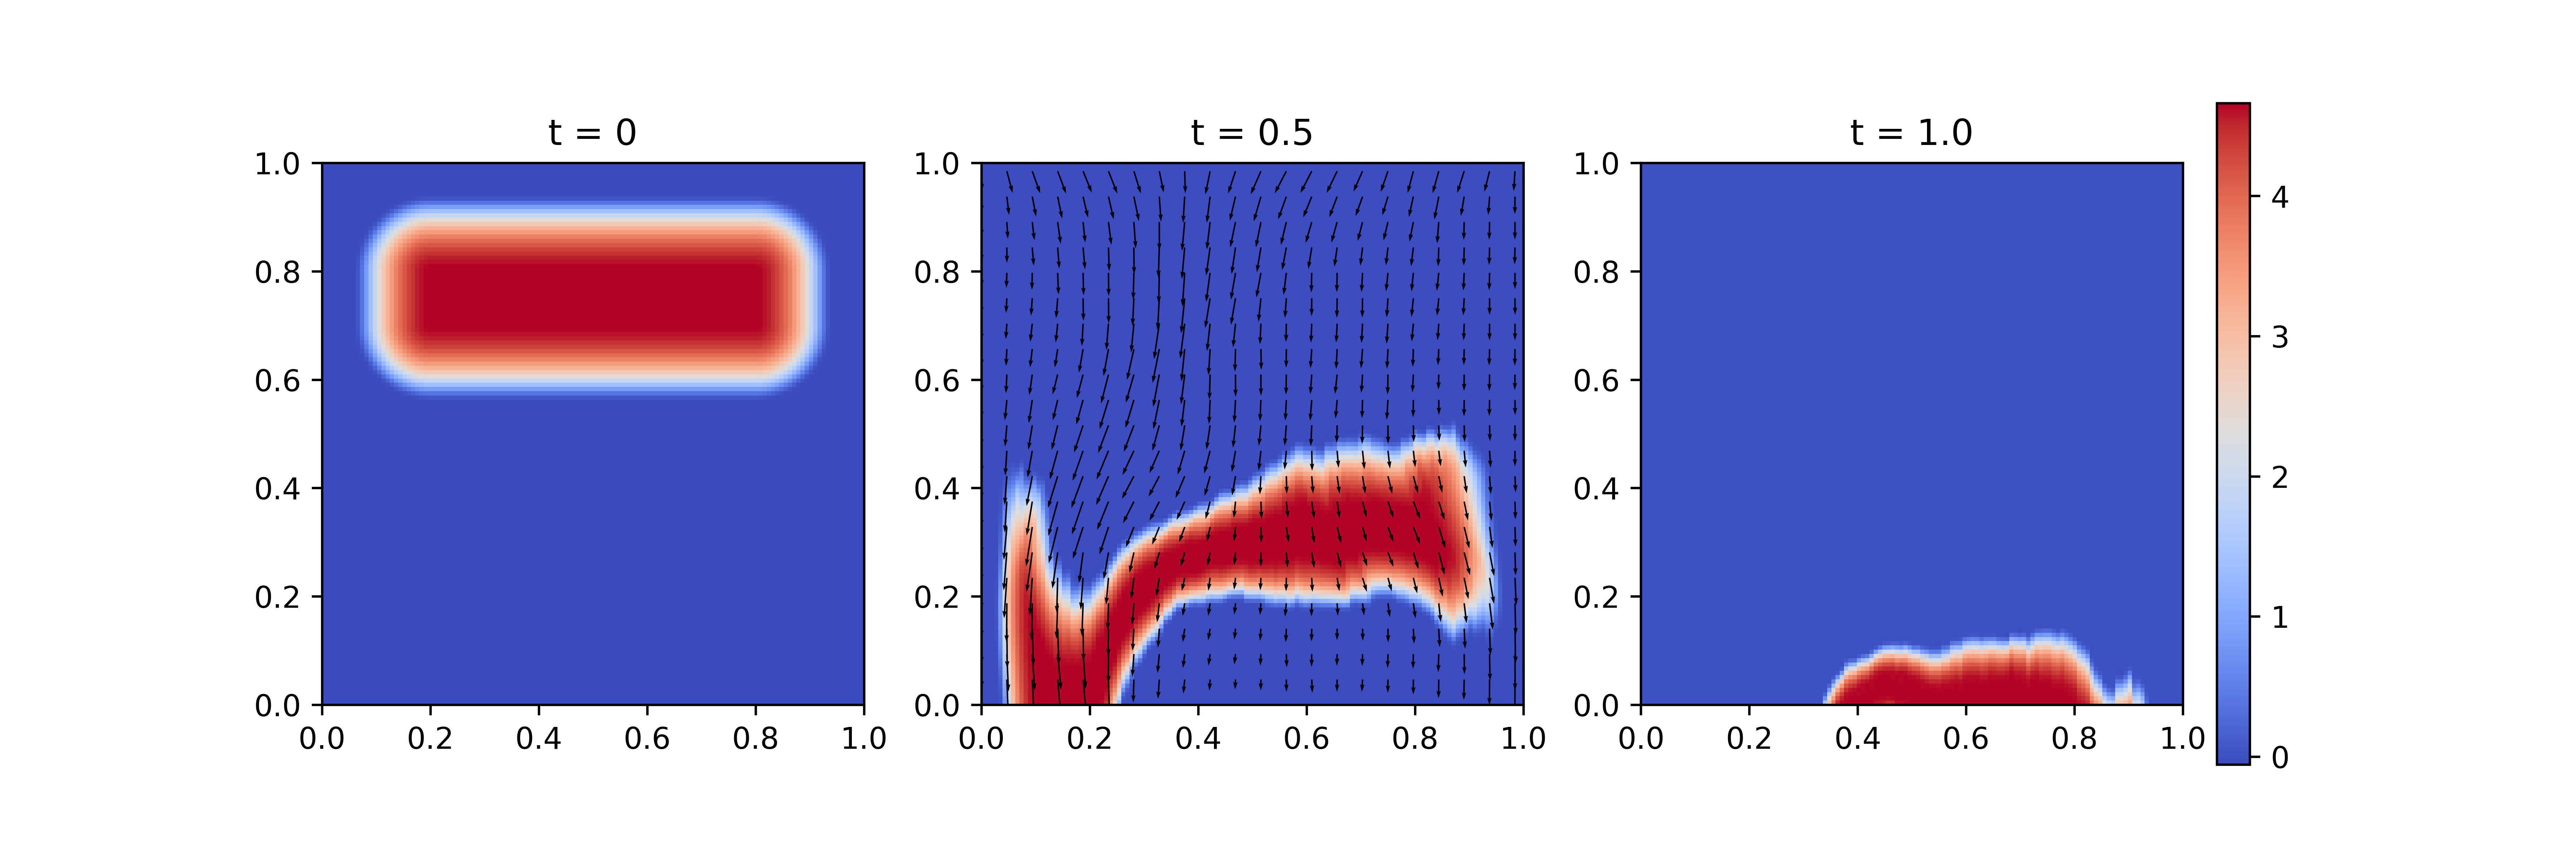
\includegraphics[width=\textwidth]{plots/solution3.png} 
\end{figure}
Die Abbildung links zeigt die Anfangsbedingung zum Zeitpunkt $ t=0 $, in der Mitte ist ein Zwischenschritt der Lösung (zum Zeitpunkt $ t=0.5 $ zu sehen) sowie das zum Sample zugehörige Flussvektorfeld zu sehen. Wir wollen an dieser Stelle noch einmal darauf hinweisen, dass wir das Flussvektorfeld als Lösung eines statischen Problems erhalten. Insbesondere ist also das Flussvektorfeld nicht zeitabhängig und könnte gleichermaßen auch bei Anfangs- und Endzustand eingezeichnet werden. 
Wir berechnen diesen Erwartungswert nun gemäß Abschnitt 6 mit der Multilevel Monte Carlo Methode für die Startwerte $ l_0 = 4, L_0 = 7, N_0 = \{n_4,\dots,n_7\} = \{16,8,4,2\} $und $ \epsilon \in \{0.01,0.005,0.003,0.001\} $.
\subsubsection{Verarbeiten und Darstellen von Vtk-Dateien}
In M++ werden zur Speicherung von Gitterdaten sogenannte Vtk-Dateien genutzt. Alle obigen sowie noch folgende Schaubilder wurden aus diesen Vtk-Dateien generiert. Dafür wurden im Rahmen der Thesis einzelne Module in Python implementiert, welche den Umgang mit diesen Vtk-Dateien erleichtern. 
\begin{figure}[H]
	\centering
	\captionabove{Überblick über implementierte Module}
	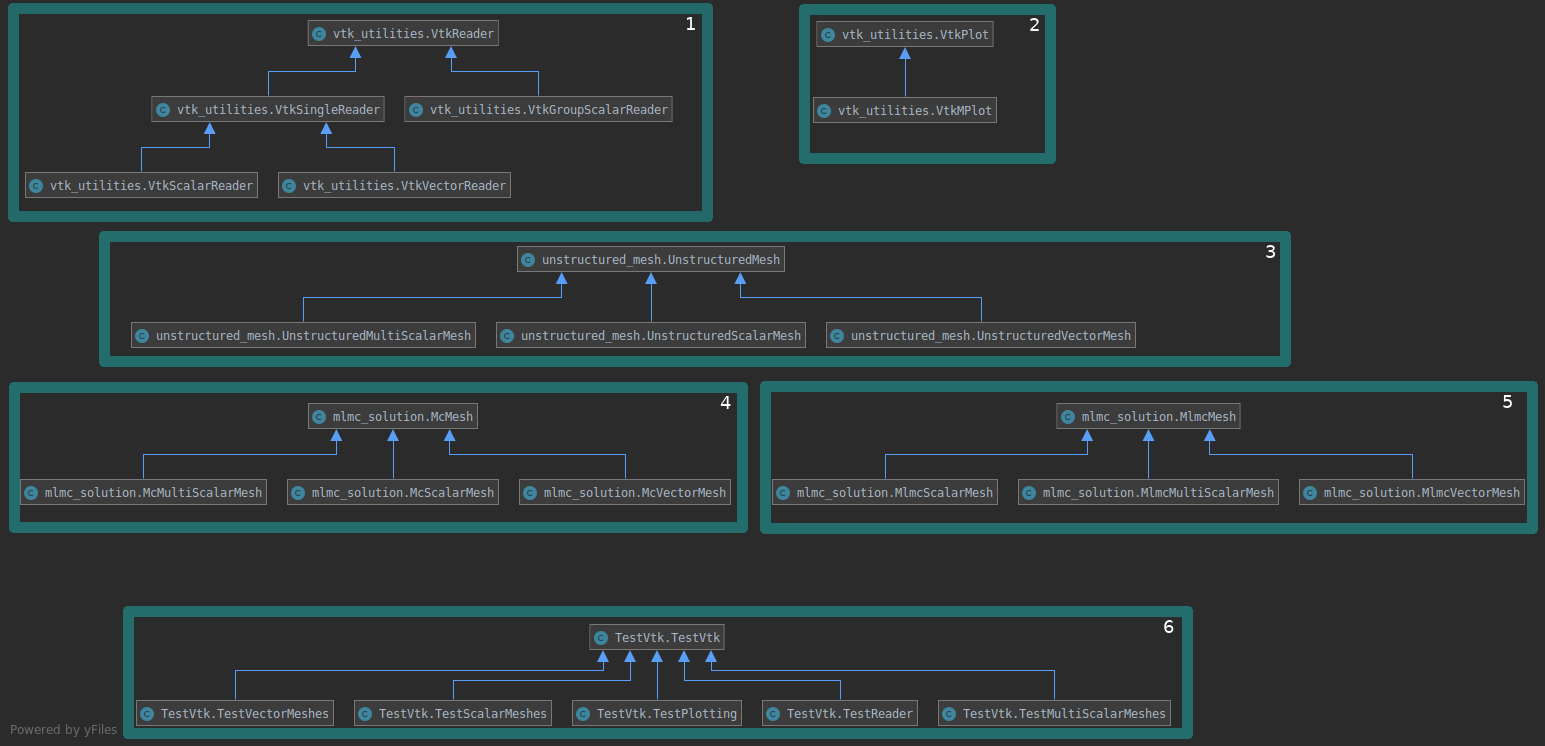
\includegraphics[width=\textwidth]{plots/klassenuml2.png} 
\end{figure}
Wie oben anhand der Klassenstrukturen dargestellt, können die Module in 6 Gruppen unterteilt werden. Gruppe 1 ermöglicht auf Grundlage des externen Moduls 'vtk' \cite{sitevtk} das Lesen von Vtk Dateien. Insbesondere ist es Möglich die Gitterdaten in sogenannten 'numpy-Arrays' zu exportieren. 
Gruppe 2 implementiert ein Interface zum Erstellen verschiedener Schaubilder aus den eingelesen Vtk Dateien. Im später im Appendix beigefügten Notebook und den entsprechenden Skripten im Hintergrund sind einige exemplarische Beispiele vorhanden. Außerdem wurde alle Schaubilder dieser Thesis über dieses Interface erstellt.
In Gruppe 3 werden die eingelesenen Arrays wieder als 'UnstructuredMesh' aufgefasst. Die Lösungen des Transportproblems selbst besteht aufgrund der Zeitabhängigkeit aus mehreren Gittern. Deshalb fassen wir diese als 'UnstructuredMultiScalarMesh' auf. Das Flussvektorfeld hingegen trägt als Daten Vektoren in jeder Zelle und wird deshalb als 'UnstructuredVectorMesh' betrachtet. Diese objektorientierte Unterteilung zieht sich bis auf Gruppe 2 durch alle Gruppen und ermöglicht den Umgang mit einzelnen Gittern und Skalaren, beispielsweise die Permeabilität des Bodens, mit einzelnen Gittern und Vektordaten, wie etwa das Flussvektorfeld, oder aber einer ganzen Gruppe von Gittern mit Skalaren, womit sich die zeitabhängige Lösung darstellen lässt. Wir können so die Lösungen der Samples als Gitterdaten auffassen und bearbeiten. Insbesondere wurden beispielsweise die Addition und Subtraktion von Gitterdaten implementiert, welche für Generierung von weiteren Gittern nach Vorbild der im Experiment durchgeführten Monte Carlo und Multilevel Monte Carlo Methoden unabdingbar sind. Unter anderem wurde dafür auch eine 'Upscale'-Methode entworfen, welche es ermöglicht unterschiedlich feine Quadratgitter miteinander zu verrechnen.
Gruppe 4 und 5 kombinieren die von M++ während des Experiments abgespeicherten Vtk Dateien wie oben beschrieben. Im Folgenden nennen wir die so (in Form von Gitterdaten) erzeugte Lösung auch 'MLMC-Lösung'.
Gruppe 6 dient dem Testen der anderen Gruppen in der Form sogenannter 'UnitTests'.
Der Code und weitere zusätzliche Informationen sind auch im zugehörigen Github-Repository \cite{githubvtk} zu finden. Das Notebook und die in das MLMC Framework eingearbeiteten Skripte finden sich auch unter \cite{branchMLMCTP}.

\subsection{Ergebnisse}
\subsubsection{Konvergenztest}
Bevor wir auf die Ergebnisse des eigentlichen Experiments eingehen, wollen wir einen kurzen Blick auf die Ergebnisse des Konvergenztests werfen. Dieser Test ist dafür da, die Annahmen welche wir unter Anderem für \eqref{MLMCTheorem} getroffen hatten, für unser konkretes Problem nachzuweisen.

%\noindent\begin{tabular}{|p{0.15\q}|p{0.55\q}|p{1.4\q}|p{1.05\q}|p{1.35\q}|p{1.25\q}|p{0.9\q}|p{1.35\q}|}
%	\hline
%	$ l $   &  $ M $  &  $ \mathbb{E}[Q_f-Q_c] $  &   $ \mathbb{E}[Q_f] $ &  $ \mathbb{V}[Q_f-Q_c] $   &   $ \mathbb{V}[Q_f] $ &  kurtosis    &    cost\\
%	\hline
%	4 & 4374&    0.224298 &   0.224298&   0.0169387 &  0.0169387  &   2.75002 &     294912 \\
%	5  &  59 & 0.00141127  &  0.231847 & 2.14581e-05 &  0.0239913  &   2.59309 & 2.3593e+06\\
%	6   &  5  &0.000726783  &  0.104317 & 9.88656e-07 & 0.00614564  &   1.66323 &1.88744e+07\\
%	\hline
%	\multicolumn{2}{|c|}{$ \mathbb{E}[Q] $ }  &  \multicolumn{2}{c|}{MLMC Cost}   & \multicolumn{2}{c|}{$ l $}  &    \multicolumn{2}{c|}{$ M$} \\
%	\hline
%	\multicolumn{2}{|c|}{0.226436} & \multicolumn{2}{c|}{1.52352e+09  } &  \multicolumn{2}{c|}{   4 5 6 }     & \multicolumn{2}{c|}{4374 59 5}    \\
%	\hline 
%\end{tabular}\\


Außerdem lassen sich auf Grundlage dieser Daten die Konvergenzparameter und später im Experiment auch einzelne Fehlerkomponenten abschätzen. 
Wir schätzen an dieser Stelle $ \alpha $, also den Exponent der schwachen Konvergenz des Verfahrens, durch den Logarithmus der Steigung der lineare Regressionsgerade der Erwartungswerte $ \mathbb{E}[Q_f - Q_c] $ gegenüber der Level. Anzumerken ist hierbei dass auf dem Basislevel, hier Level 4, keine Differenz in Spalte 3 und 5 angegeben werden kann, da auf dem Basislevel nur einzelne Samples ohne gröberes Vergleichssample betrachtet werden. Stattdessen werden hier in Spalte 3 und 5 ebenfalls wie in Spalte 4 und 6 der einzelne Erwartungswert bzw. die einzelne Varianz angegeben. Bei der Schätzung von $ \alpha $ wird deshalb das Basislevel nicht einbezogen.
Den Exponenten des Rückgangs der Varianz $ \beta $ schätzen ähnlich wie $ \alpha $ als Logarithmus der Steigung einer Regressionsgeraden, diesmal über den den Rückgang der empirischen Varianzdifferenzen  $ \mathbb{V}[Q_f-Q_c] $ gegen die entsprechenden Level. Die Kosten in der letzten Spalte selbst werden während des Experiments über die Anzahl der Freiheitsgrade des zugrunde liegenden linearen Gleichungssystems abgeschätzt. 
Auf Grundlage dieser geschätzten Kosten lässt sich dann genauso $ \gamma $ als Logarithmus der Steigung einer entsprechenden linearen Regression über die pro Level erwarteten Kosten $ \mathbb{E}[C_l] $ bestimmen. Da in unserer Schätzung die Kosten der Samples auf einem Level konstant ist, stimmt dieser Erwartungswert mit den Kosten jedes einzelnen Samples überein.  
Konkret erhalten wir mit obigen Daten: 

\begin{align*}
\alpha &= \\
\beta &= \\
\gamma &= \\
\end{align*}
\subsubsection{Einige Beispielsamples}
Um einen ersten Eindruck über die berechneten Samples zu gewinnen, ist es hilfreich einige Beispielsamples zu betrachten. Im Experiment werden wir Samples auf den Levels $ 4,5,6 $ und $ 7 $ betrachten. Im Folgenden sind daher zu diesen Levels je ein Beispielsample dargestellt.
\begin{figure}[H]
	\centering
	\captionabove{Verlauf der Konzentration eines Samples auf Level $ l_0 = 4 $}
	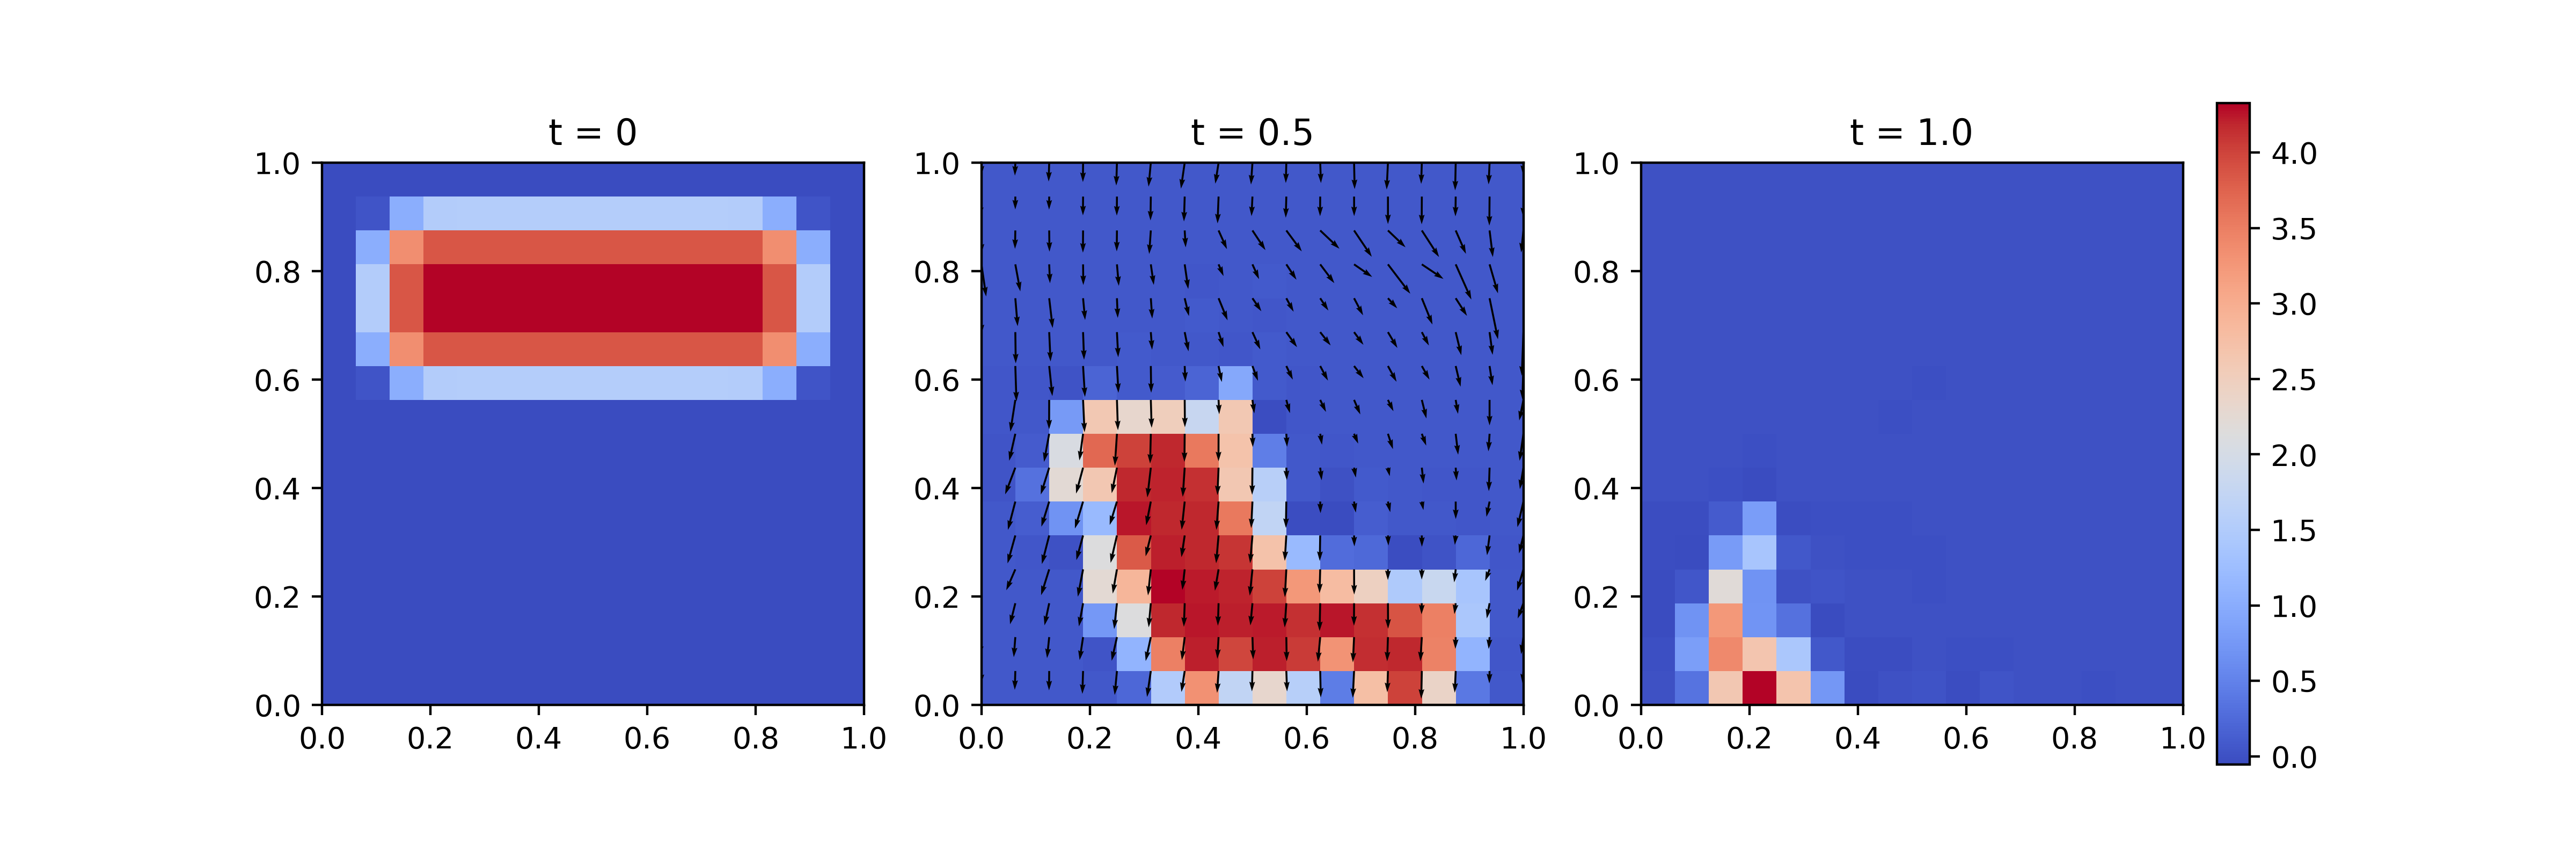
\includegraphics[width=\textwidth]{plots/sample_4_1.png} 
\end{figure}
\begin{figure}[H]
	\centering
	\captionabove{Verlauf der Konzentration eines Samples auf Level $ l_1 = 5 $ und des zugehörigen Vergleichssamples auf Level $ l_0 = 4 $}
	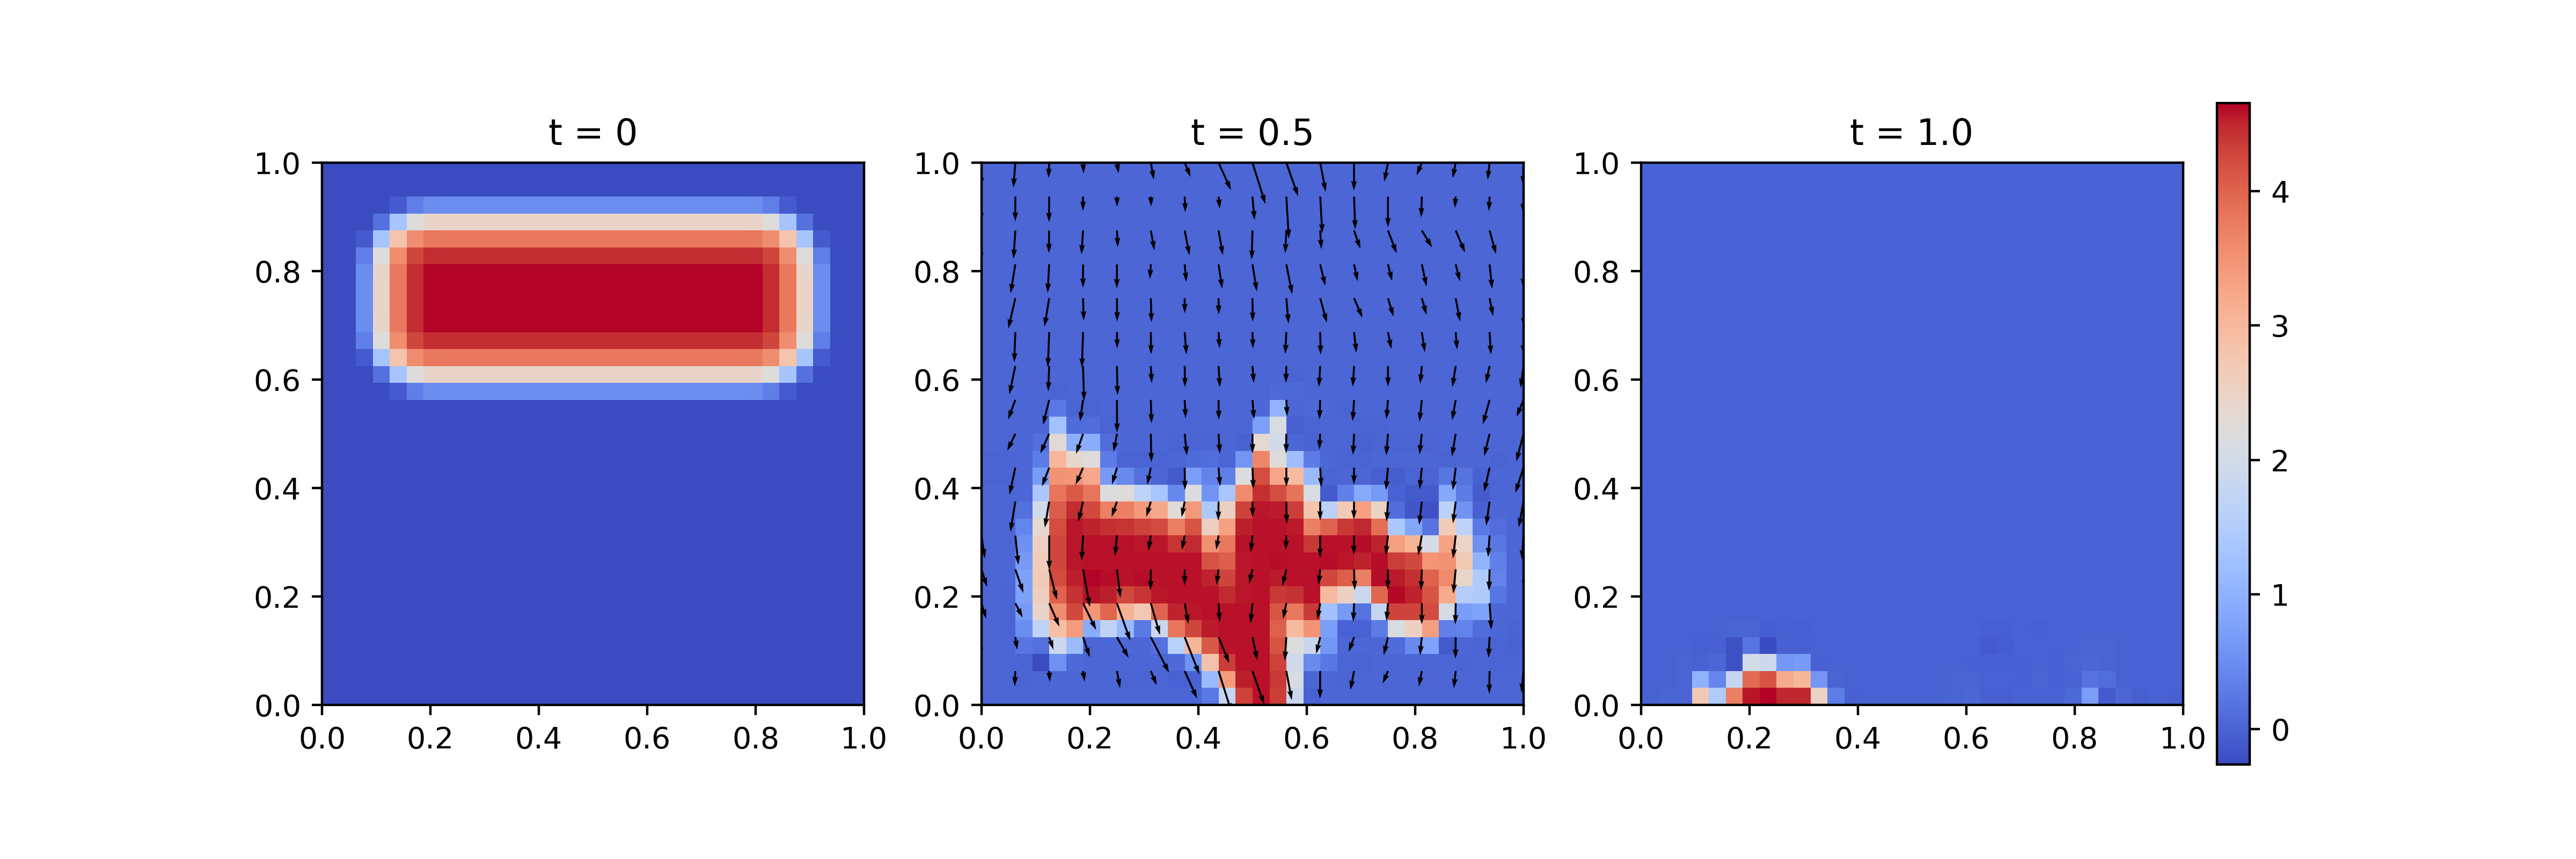
\includegraphics[width=\textwidth]{plots/sample_5_1.png} 
	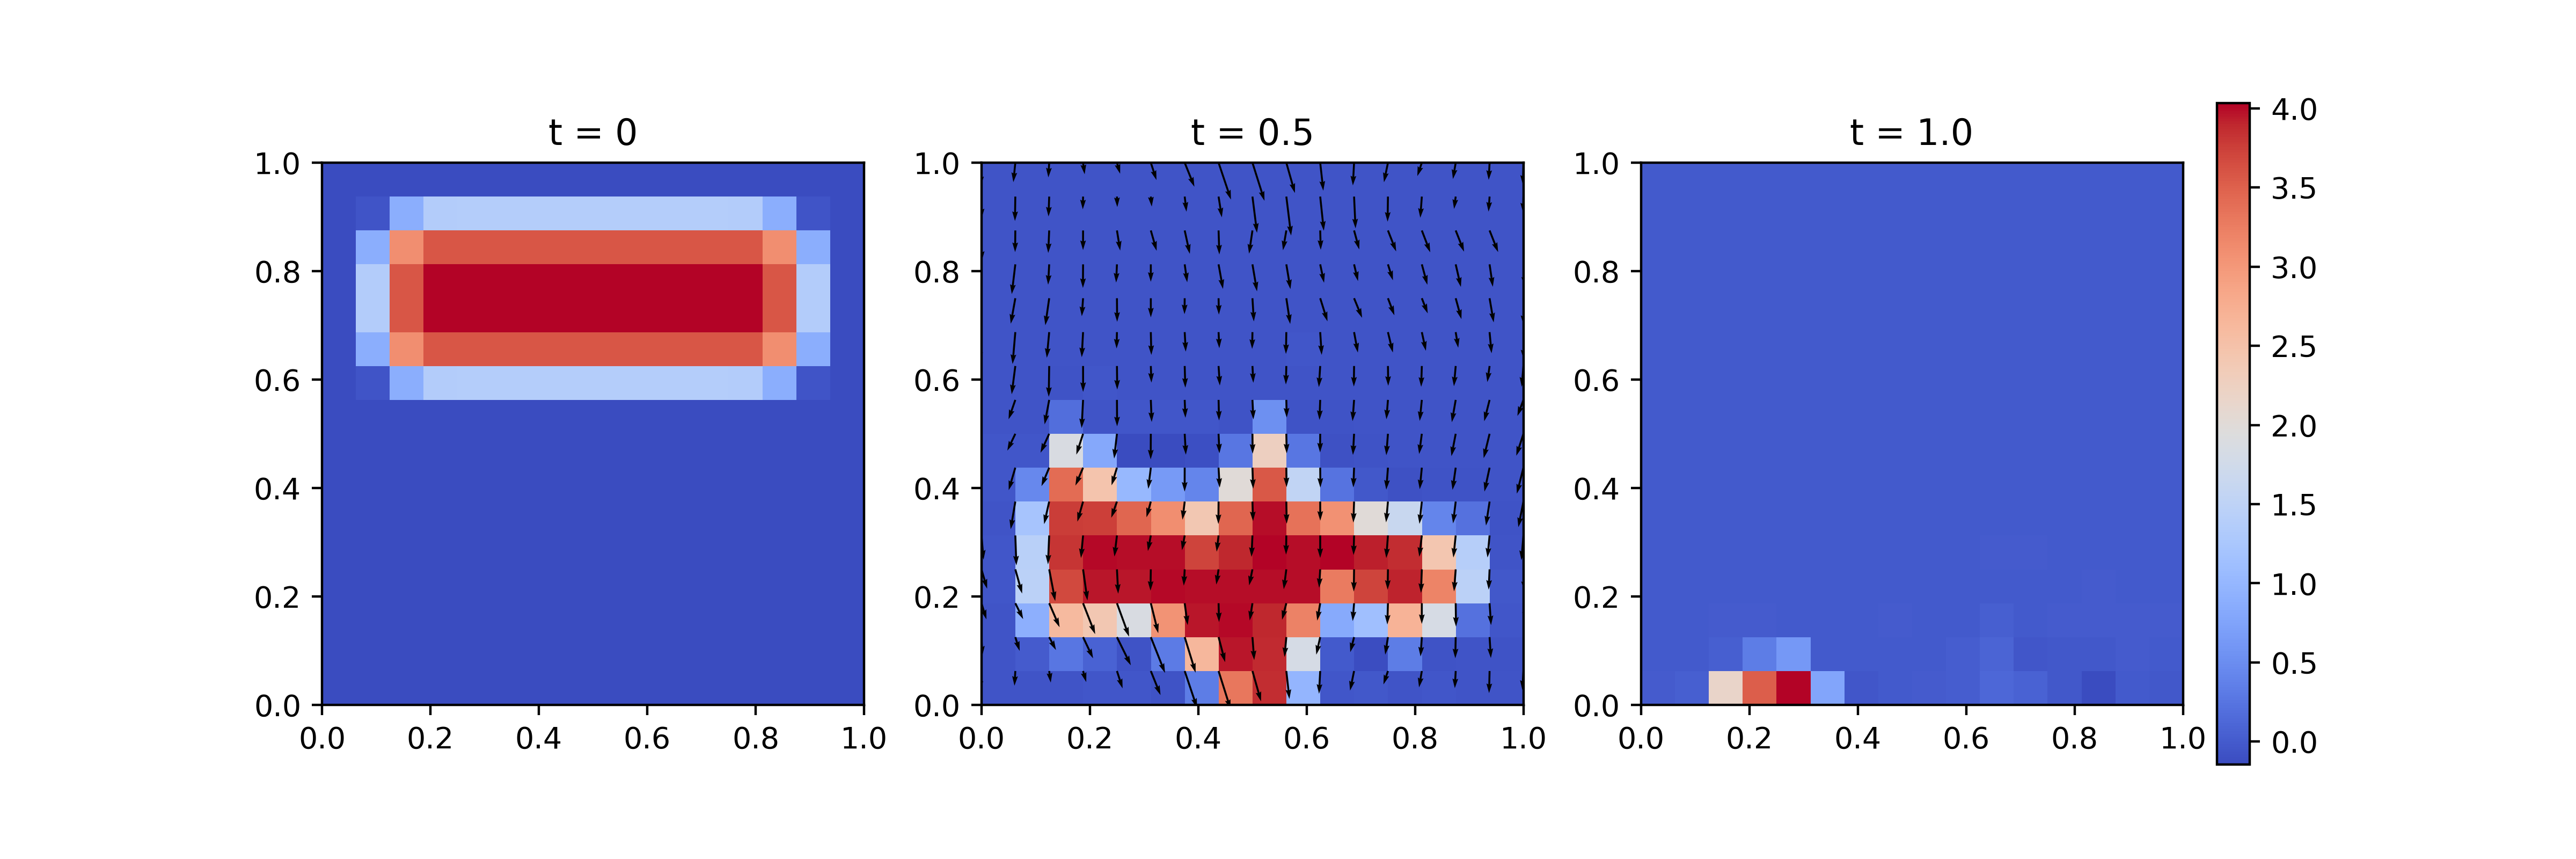
\includegraphics[width=\textwidth]{plots/sample_coarse_5_1.png} 
\end{figure}
An diesem direkten Vergleich sieht man sehr schön, dass sich die beiden Vergleichssamples zwar im Level unterscheiden, aber sich auf dasselbe Zufallsereignis $ \omega_i $ beziehen. Noch offensichtlicher wird das, je höher das aktuell betrachtete Level ist:
\begin{figure}[H]
	\centering
	\captionabove{Verlauf der Konzentration eines Samples auf Level $ l_2 = 6 $ und des zugehörigen Vergleichssamples auf Level $ l_1 = 5 $}
	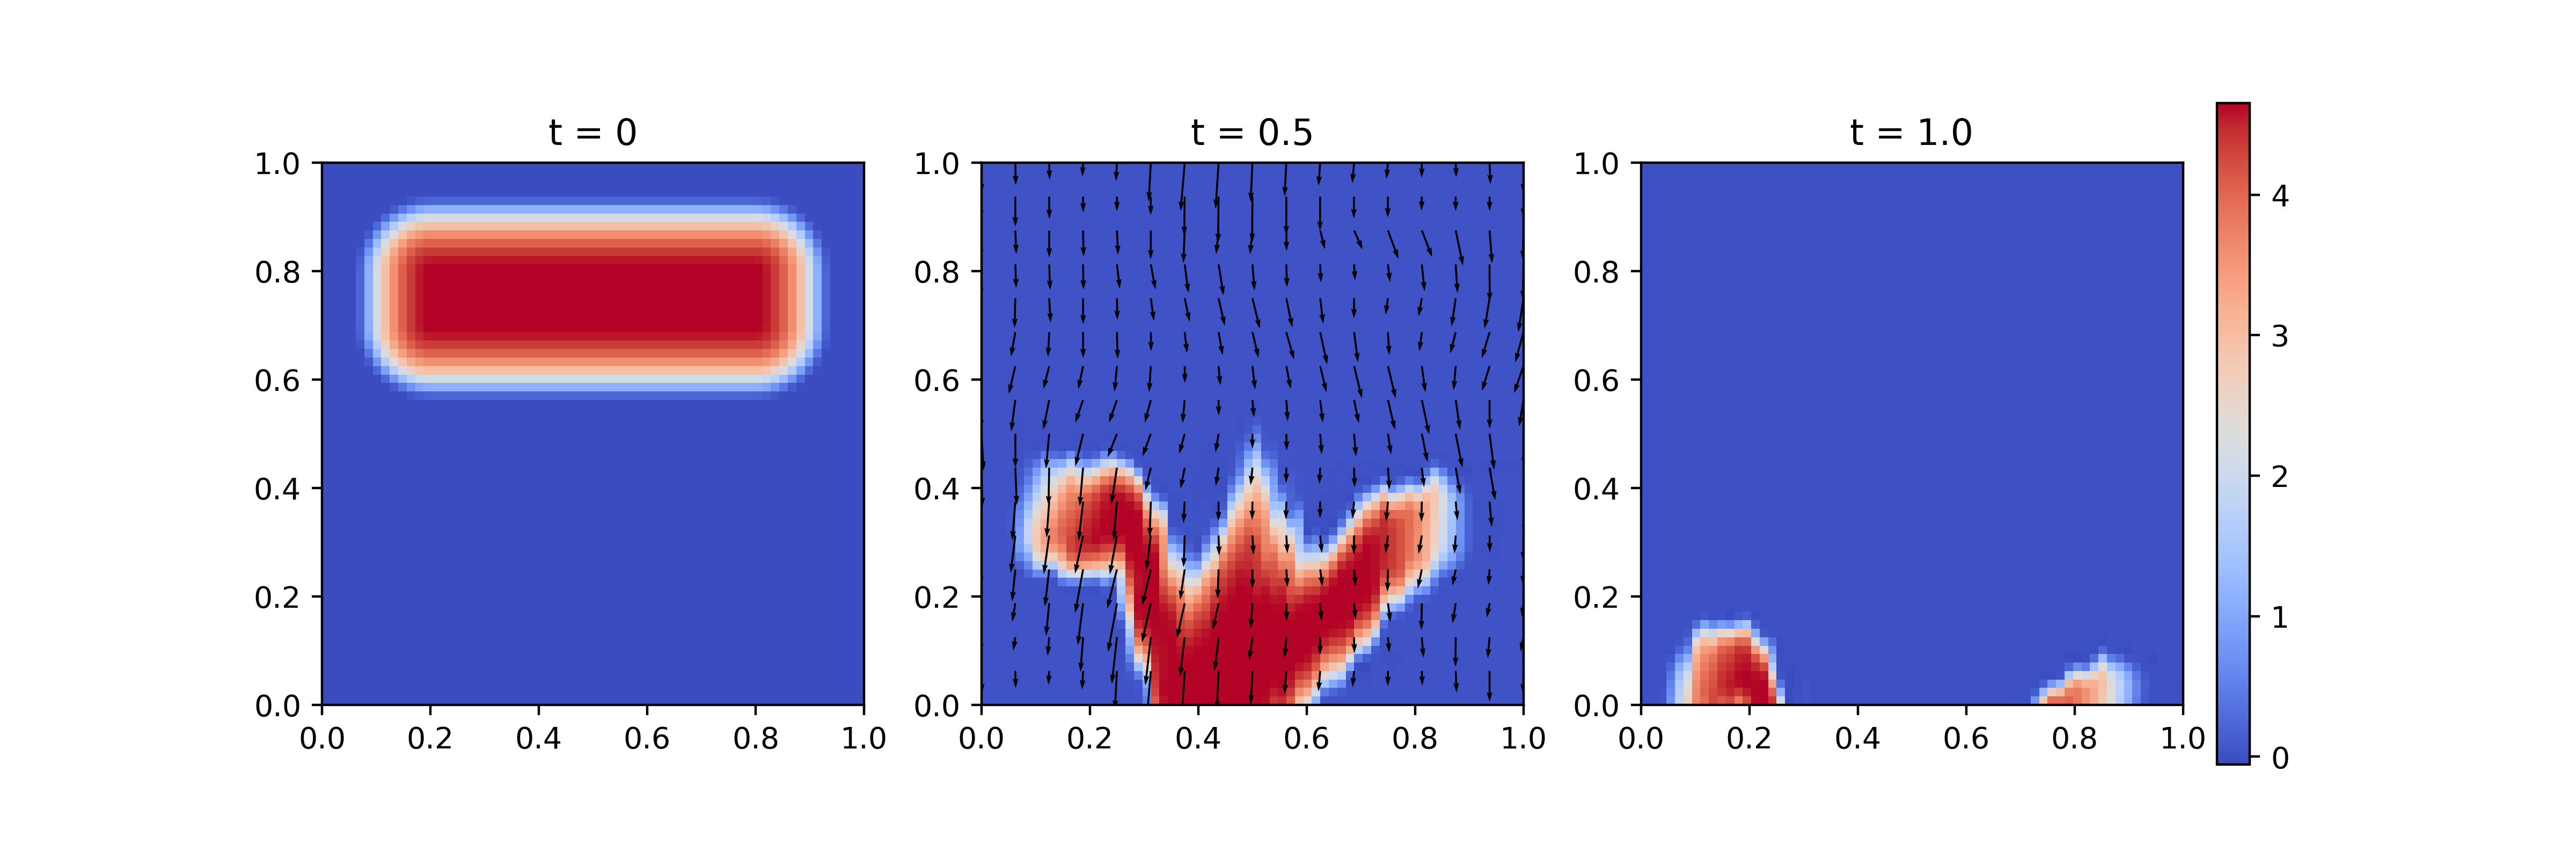
\includegraphics[width=\textwidth]{plots/sample_6_0.png} 
	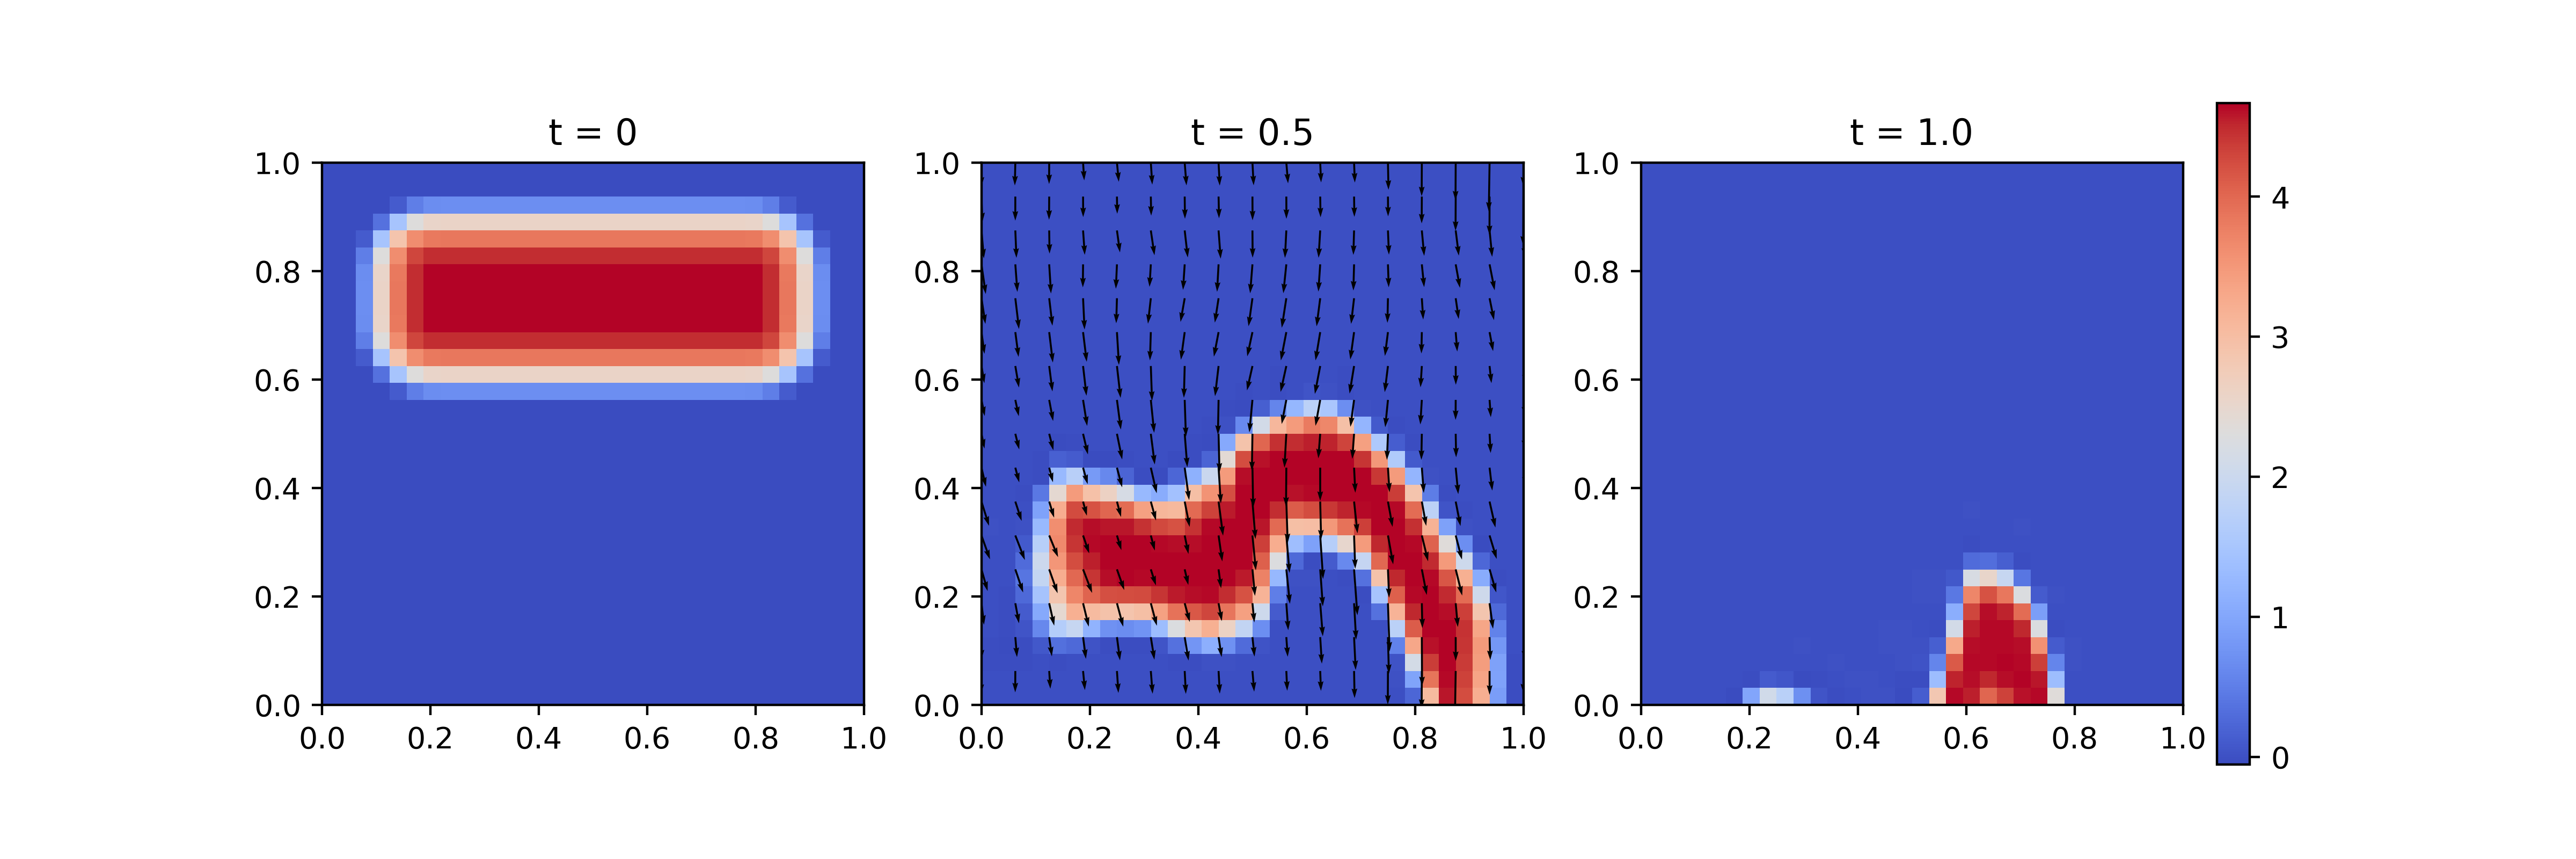
\includegraphics[width=\textwidth]{plots/sample_coarse_6_0.png} 
\end{figure}
\begin{figure}[H]
	\centering
	\captionabove{Verlauf der Konzentration eines Samples auf Level $ l_3 = 7 $ und des zugehörigen Vergleichssamples auf Level $ l_2 = 6 $}
	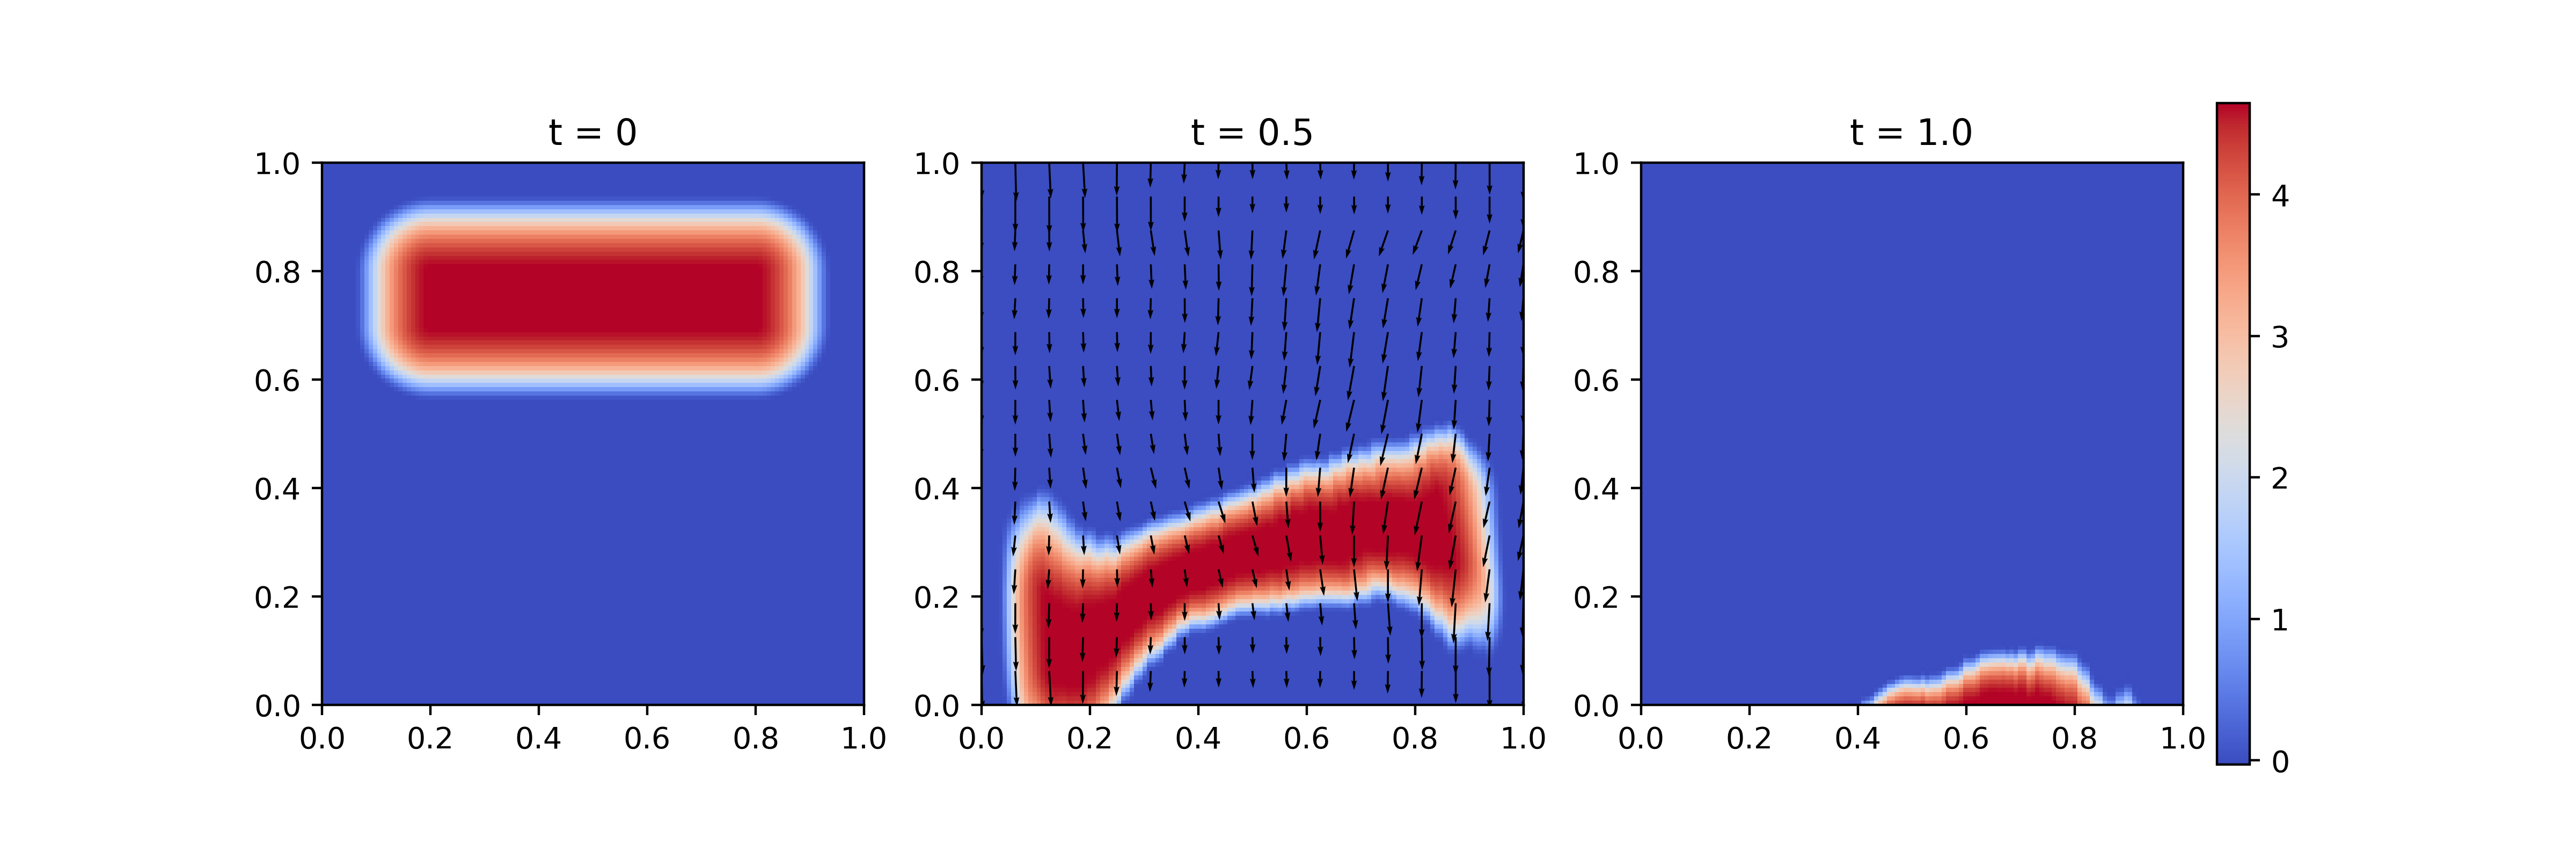
\includegraphics[width=\textwidth]{plots/sample_7_0.png} 
	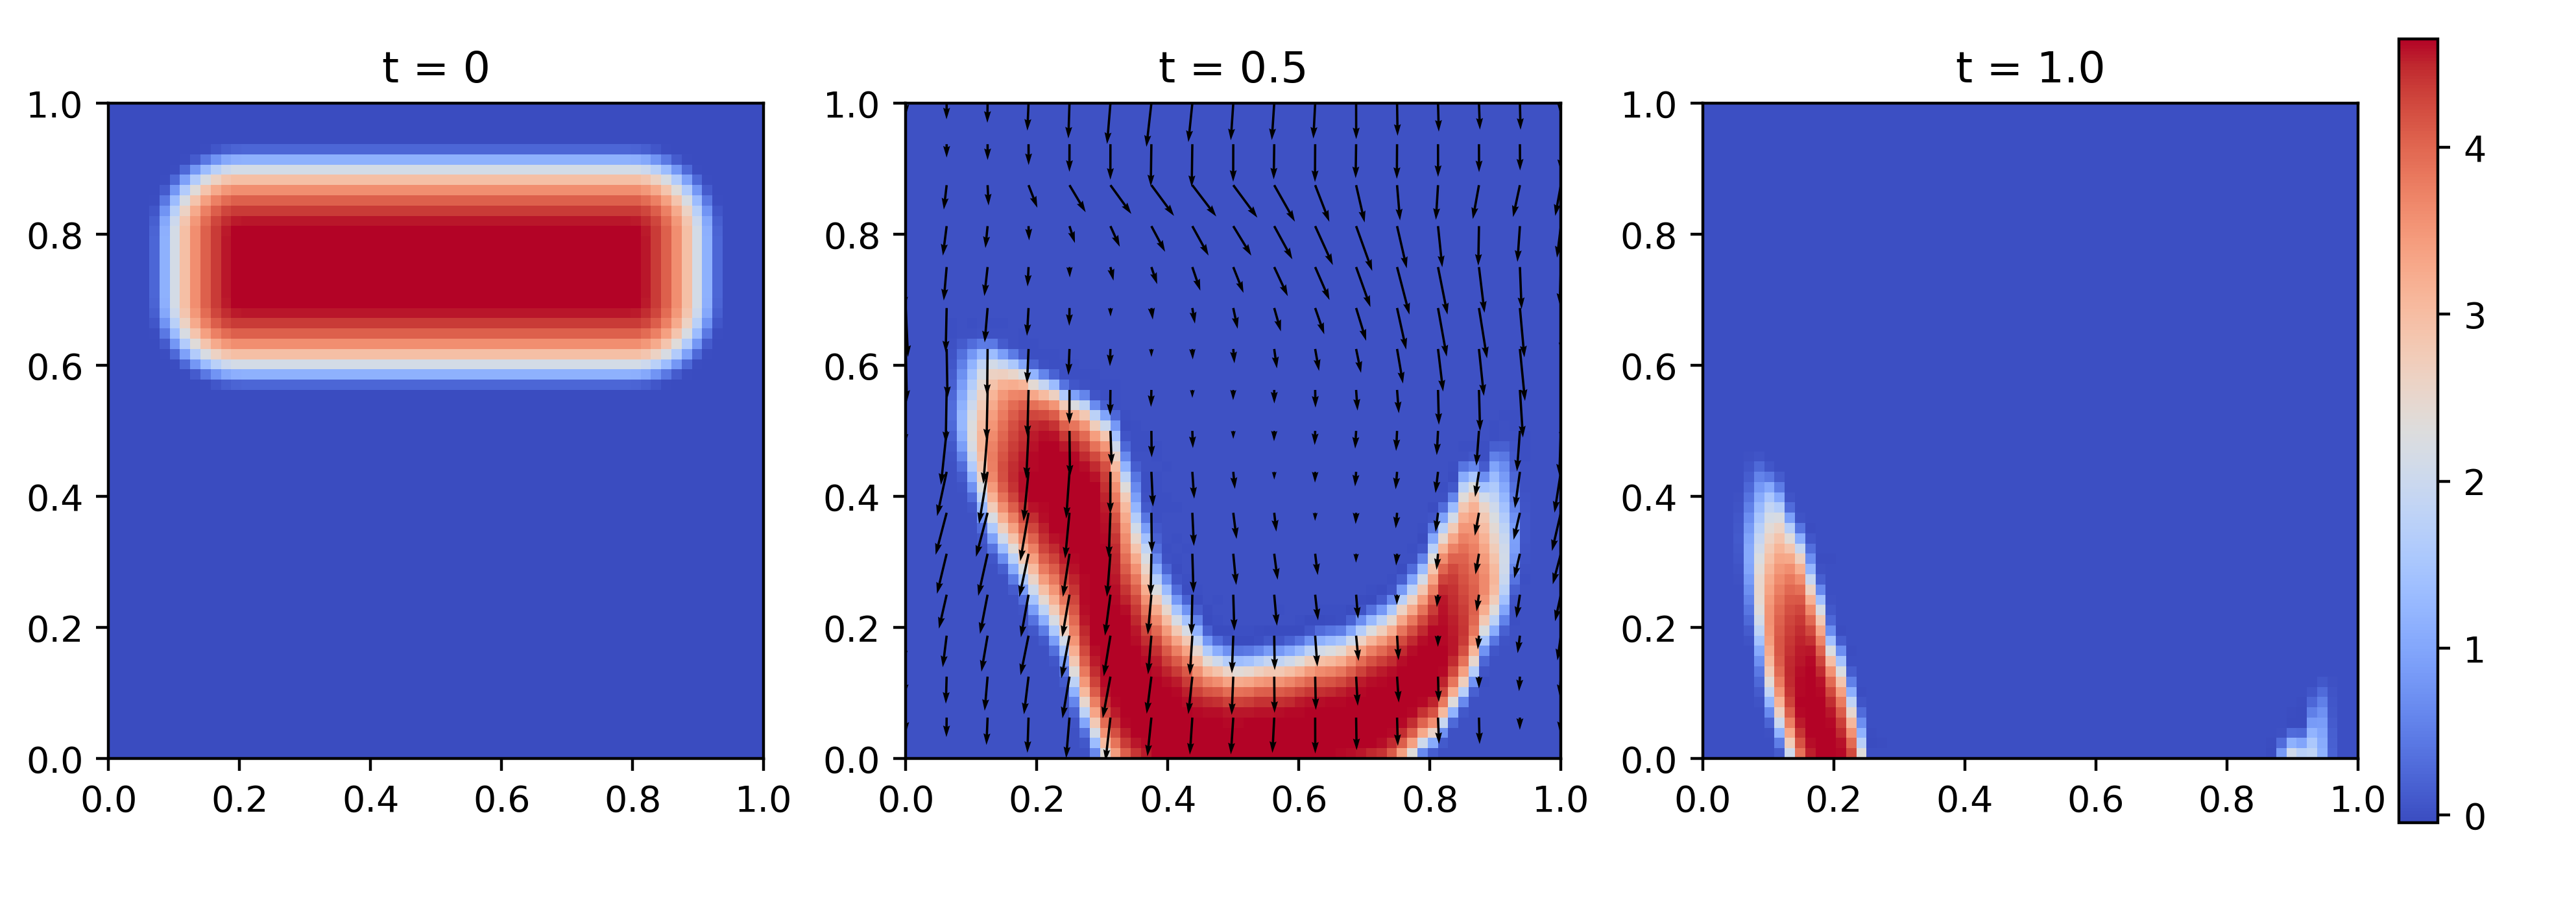
\includegraphics[width=\textwidth]{plots/sample_coarse_7_0.png} 
\end{figure}
\subsubsection{$ \epsilon=0.01 $}
Wir führen das Experiment für vier verschiedene Werte von $ \epsilon $ durch und beginnen mit dem größten Wert $ \epsilon=0.01 $. Wir erhalten: 

\newlength\q
\setlength\q{\dimexpr .125\textwidth -2.0\tabcolsep}
\noindent\begin{tabular}{|p{0.15\q}|p{0.55\q}|p{1.4\q}|p{1.05\q}|p{1.35\q}|p{1.25\q}|p{0.9\q}|p{1.35\q}|}
	\hline
	$ l $   &  $ M $  &  $ \mathbb{E}[Q_f-Q_c] $  &   $ \mathbb{E}[Q_f] $ &  $ \mathbb{V}[Q_f-Q_c] $   &   $ \mathbb{V}[Q_f] $ &  kurtosis    &    cost\\
	\hline
	4 &  378 &   0.225017  &  0.225017 &  0.0161076 &  0.0161076  &    2.9913&      294912 \\
	5 &    6 & 0.00142942  &  0.261486 &2.27982e-05 &  0.0158132  &   3.92345&  2.3593e+06 \\
	6 &    2 & 0.00132101  &  0.106957 &4.09672e-07 & 0.00590853  &         1& 1.88744e+07 \\
	7 &    2 & 5.6257e-05  &  0.125627 &      1e-10 &0.000783613  &  0.110661& 1.50995e+08 \\
	\hline
	\multicolumn{2}{|c|}{$ \mathbb{E}[Q] $ }  &  \multicolumn{2}{c|}{MLMC Cost}   & \multicolumn{2}{c|}{$ l $}  &    \multicolumn{2}{c|}{$ M$} \\
	\hline
	\multicolumn{2}{|c|}{0.227824} & \multicolumn{2}{c|}{4.65371e+08  } &  \multicolumn{2}{c|}{   4 5 6 7}     & \multicolumn{2}{c|}{  378 6 2 2}    \\
	\hline 
\end{tabular}\\

Wie bereits oben beim Konvergenztest können wir auch auf Grundlage der konkreten Daten des Experiments die Konvergenzparameter $ \alpha, \beta $ und  $ \gamma $ schätzen:
\begin{align*}
\alpha  &=     2.33362   \\
\beta   &=    8.89928   \\
\gamma  &=    3  \\
\end{align*}
Zudem können wir auch die einzelnen Fehlerkomponenten abschätzen, diese Fehlerschätzung wird auch im Algorithmus selbst vorgenommen. So lässt sich der statistische Fehler durch \[
\text{statErr} \leq \sqrt{\sum_l   \frac{\mathbb{V}[Q_f-Q_c]}{M_l}} \ . \] 
Den numerischen Fehler können wir über einen Romberg Fehlerschätzer abschätzen und nutzen dabei die Abschätzung \[ \left| \mathbb{E}[Q_f-Q_c] \right| < (2^{\alpha}-1)\frac{\epsilon}{2} \ . \] Mehr zu obigen Fehlerschätzern und eine Erklärung für obige Abschätzung findet sich in \cite{giles_2015}.
Wir erhalten an dieser Stelle so: 
\begin{align*}
\text{numErr}  &=  0.000163463   \quad \text{(geschätzter numerischer Fehler)}\\
\text{statErr} &= 0.00682769  \quad  \text{(geschätzter statistischer Fehler)}\\
\text{error}   &= 0.00699115   \quad  \text{(geschätzter Gesamtfehler)}\\
\end{align*}


\subsubsection{$ \epsilon=0.005 $}

\noindent\begin{tabular}{|p{0.15\q}|p{0.55\q}|p{1.4\q}|p{1.05\q}|p{1.35\q}|p{1.25\q}|p{0.9\q}|p{1.35\q}|}
	\hline
	$ l $   &  $ M $  &  $ \mathbb{E}[Q_f-Q_c] $  &   $ \mathbb{E}[Q_f] $ &  $ \mathbb{V}[Q_f-Q_c] $   &   $ \mathbb{V}[Q_f] $ &  kurtosis    &    cost\\
	\hline
	4 & 1539 &   0.223618  &  0.223618&    0.016789&    0.016789 &    2.86354&      294912  \\
	5  &  22 & 0.00136769  &  0.257407& 1.64094e-05&   0.0231786 &    3.11973&  2.3593e+06 \\
	6   &  2 & 0.00132101  &  0.106957& 4.09672e-07&  0.00590853 &          1& 1.88744e+07 \\
	7    & 2 & 5.6257e-05  &  0.125627&       1e-10& 0.000783613 &   0.110661& 1.50995e+08 \\
	\hline
	\multicolumn{2}{|c|}{$ \mathbb{E}[Q] $ }  &  \multicolumn{2}{c|}{MLMC Cost}   & \multicolumn{2}{c|}{$ l $}  &    \multicolumn{2}{c|}{$ M$} \\
	\hline
	\multicolumn{2}{|c|}{0.226363} & \multicolumn{2}{c|}{8.45513e+08  } &  \multicolumn{2}{c|}{  4 5 6 7 }     & \multicolumn{2}{c|}{1539 22 2 2}    \\
	\hline 
\end{tabular}\\
\begin{align*}
\alpha  &=     2.30178   \\
\beta   &=    8.66208   \\
\gamma  &=    3   \\
\text{numErr}  &=  0.00016804   \quad \text{(geschätzter numerischer Fehler)}\\
\text{statErr} &= 0.00344381  \quad  \text{(geschätzter statistischer Fehler)}\\
\text{error}   &= 0.00361185  \quad  \text{(geschätzter Gesamtfehler)}\\
\end{align*}


\subsubsection{$ \epsilon=0.003 $}
\noindent\begin{tabular}{|p{0.15\q}|p{0.55\q}|p{1.4\q}|p{1.05\q}|p{1.35\q}|p{1.25\q}|p{0.9\q}|p{1.35\q}|}
	\hline
	$ l $   &  $ M $  &  $ \mathbb{E}[Q_f-Q_c] $  &   $ \mathbb{E}[Q_f] $ &  $ \mathbb{V}[Q_f-Q_c] $   &   $ \mathbb{V}[Q_f] $ &  kurtosis    &    cost\\
	\hline
	4 & 4374&    0.224298 &   0.224298&   0.0169387 &  0.0169387  &   2.75002 &     294912 \\
	5  &  59 & 0.00141127  &  0.231847 & 2.14581e-05 &  0.0239913  &   2.59309 & 2.3593e+06\\
	6   &  5  &0.000726783  &  0.104317 & 9.88656e-07 & 0.00614564  &   1.66323 &1.88744e+07\\
	\hline
	\multicolumn{2}{|c|}{$ \mathbb{E}[Q] $ }  &  \multicolumn{2}{c|}{MLMC Cost}   & \multicolumn{2}{c|}{$ l $}  &    \multicolumn{2}{c|}{$ M$} \\
	\hline
	\multicolumn{2}{|c|}{0.226436} & \multicolumn{2}{c|}{1.52352e+09  } &  \multicolumn{2}{c|}{   4 5 6 }     & \multicolumn{2}{c|}{4374 59 5}    \\
	\hline 
\end{tabular}\\

\begin{align*}
\alpha  &=    0.957394   \\
\beta   &=    4.43991   \\
\gamma  &=    3   \\
\text{numErr}  &= 0.000771696   \quad \text{(geschätzter numerischer Fehler)}\\
\text{statErr} &= 0.00210571  \quad  \text{(geschätzter statistischer Fehler)}\\
\text{error}   &= 0.00287741  \quad  \text{(geschätzter Gesamtfehler)}\\
\end{align*}


\subsubsection{$ \epsilon=0.001 $}

\noindent\begin{tabular}{|p{0.15\q}|p{0.54\q}|p{1.4\q}|p{1.05\q}|p{1.35\q}|p{1.25\q}|p{0.9\q}|p{1.35\q}|}
\hline
$ l $   &  $ M $  &  $ \mathbb{E}[Q_f-Q_c] $  &   $ \mathbb{E}[Q_f] $ &  $ \mathbb{V}[Q_f-Q_c] $   &   $ \mathbb{V}[Q_f] $ &  kurtosis    &    cost\\
\hline
4 & 44254  & 0.226394   &  0.226394 &  0.0174305   &  0.0174305  &   2.65924   &   294912    \\
5 &  755   & 0.00168666 &  0.21234  &  4.12796e-05 &  0.0198136  &   3.68994   &   2.3593e+06\\
6 &   58   & 0.000869439&  0.20211  &  1.83935e-06 &   0.020755  &   3.80032   &   1.88744e+07 \\
7 &    5   & 7.68982e-05&    0.218324&  9.1227e-09&  0.00718929   &  2.45257 &1.50995e+08 \\
\hline 
 \multicolumn{2}{|c|}{$ \mathbb{E}[Q] $ }  &  \multicolumn{2}{c|}{MLMC Cost}   & \multicolumn{2}{c|}{$ l $}  &    \multicolumn{2}{c|}{$ M$} \\
\hline
 \multicolumn{2}{|c|}{0.229027} & \multicolumn{2}{c|}{1.6682e+10  } &  \multicolumn{2}{c|}{  4 5 6 7 }     & \multicolumn{2}{c|}{44254 755 58 5}    \\
\hline 
\end{tabular}\\


\begin{align*}
	\alpha  &=    2.22754   \\
	\beta   &=    6.07184   \\
	\gamma  &=    3   \\
\text{numErr}  &= 0.000118023   \quad \text{(geschätzter numerischer Fehler)}\\
\text{statErr} &= 0.000694324  \quad  \text{(geschätzter statistischer Fehler)}\\
\text{error}   &= 0.000812347  \quad  \text{(geschätzter Gesamtfehler)}\\
\end{align*}

Betrachten wir die MLMC Kosten gegen die Genauigkeit $ \epsilon $ erhalten wir so:
\begin{figure}[H]
	\centering
	\captionabove{Vergleich über $ \epsilon $}
	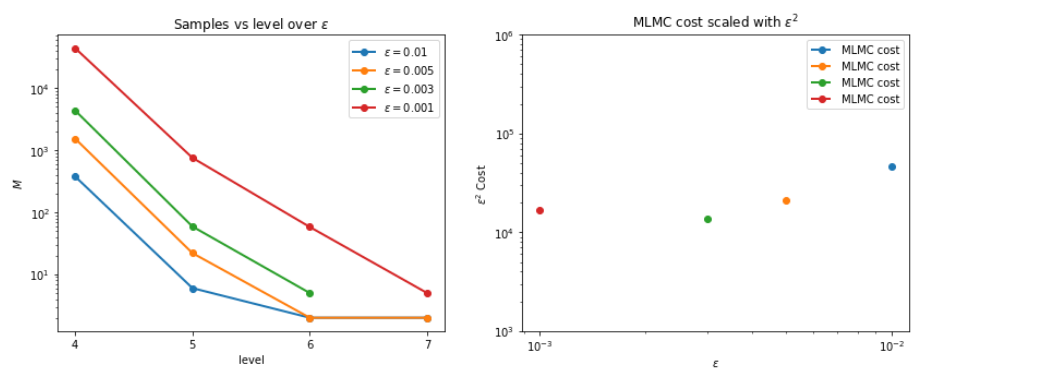
\includegraphics[width=\textwidth]{plots/mlmctable.png} 
\end{figure}


\subsection{MLMC Lösung}
Zu guter Letzt ist es uns zudem über die Verarbeitung der gespeicherten VTK-Dateien möglich, die berechneten Lösungen, welche uns in Form von Gitterdaten vorliegen zu einer MLMC-Lösung zu kombinieren. Dazu addieren wir die Gitterdaten der Samples auf dem jeweiligen Level, subtrahieren überall außer im Basislevel $ 4 $ jeweils die Summe der Coarse-Samples, skalieren mit der Anzahl der betrachteten Samples und kombinieren anschließend die so entstandenen Monte-Carlo Lösungen zu einer Multilevel Monte Carlo Lösung.
Einer der wichtigsten Schritte ist dabei das sogenannten "Upscaling", welches uns ermöglicht verschieden feine Gitter miteinander zu verrechnen. In unserem Fall ist dies recht einfach, da wir im Ort reguläre Gitter mit identischen Quadraten und in der Zeit eine äquidistante Zerlegung betrachten. Der zugehörige Code findet sich ebenfalls in \cite{githubvtk} in der Datei $'mlmc\_solution.py'$.
Auch zu den so entstehenden Gitterdaten können wir wieder entsprechende Schaubilder generieren:
%\begin{figure}[H]
%	\centering
%	\captionabove{MLMC-Lösung für den Durchlauf $ \epsilon = 0.001 $}
%	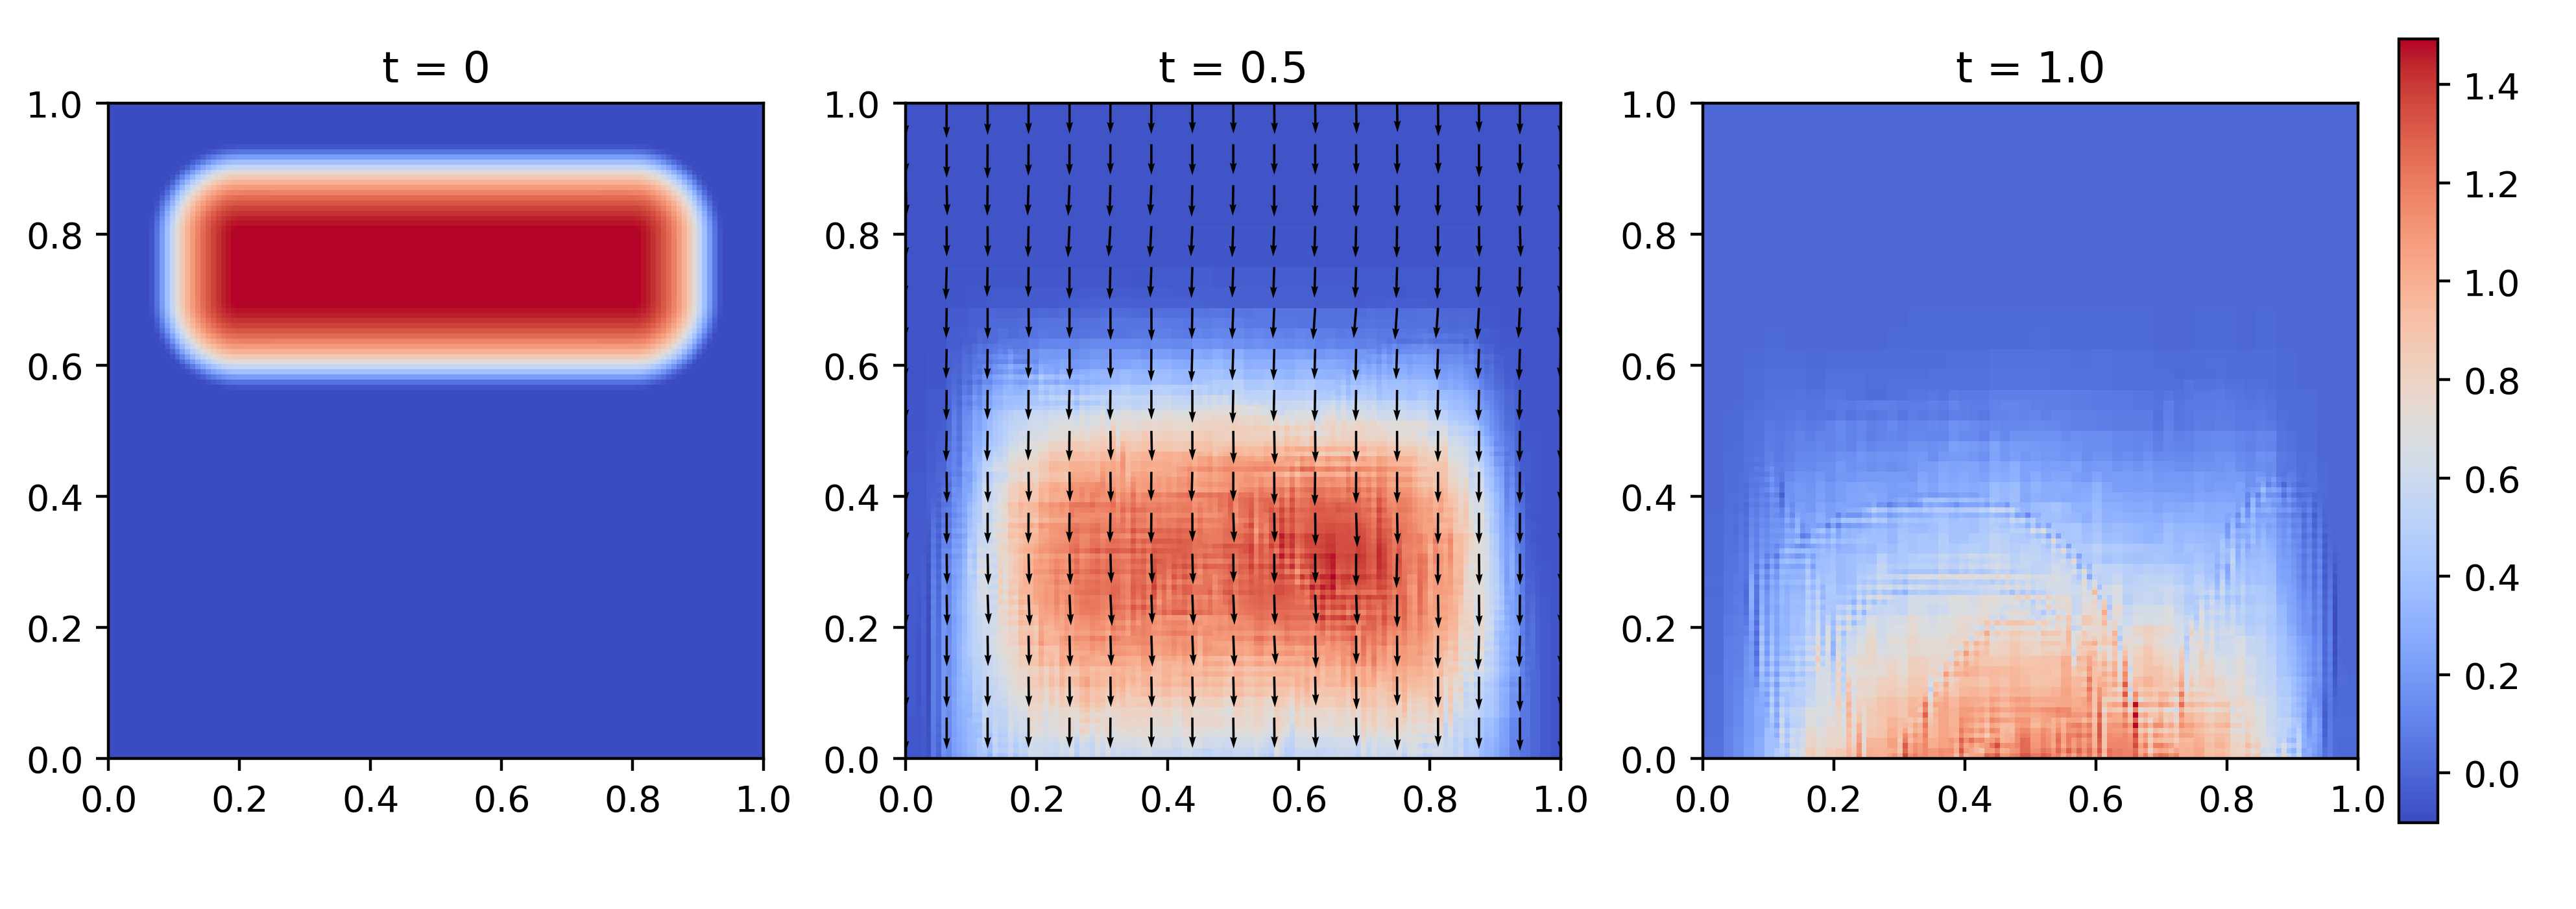
\includegraphics[width=\textwidth]{plots/mlmc.png} 
%\end{figure}



%%%%%%%%%%%%%%%%%%%%%%%%%%%%%%%%%
\newpage  % neuer Abschnitt auf neue Seite, kann auch entfallen
%%%%%%%%%%%%%%%%%%%%%%%%%%%%%%%%%
\section{Notation}
% !TeX root = bachelorarbeit.tex
Folgende Tabelle soll weder stichhaltige Definitionen festlegen, noch die gesamte Notation der Thesis bis auf den letzten Index ausarbeiten. Sie soll dem Leser eher als Orientierung dienen, welche Symbole für die verschiedenen Teilbereiche genutzt werden.

\begin{longtable}[c]{ p{0.15\textwidth} p{0.84\textwidth}}
	\hline
	Symbol    & Beschreibung   \\
	\hline
	$ \dive $ & Divergenz \\
	$ \nabla $ & Gradient \\
	$ \mathcal{D} \subset \R^d$      & Rechengebiet       \\
	$ d \in \N $      & Dimension des Rechengebietes        \\
	$ d_1, d_2 \in \N $ & Dimensionen des Integrations- und Testraumes in Beispiel \ref{mlmcbeispiel}  \\
	$ (\Omega,\mathcal{A},\mathbb{P}) $       & Wahrscheinlichkeitsraum $ \Omega $ über der $ \sigma $-Algebra $ \mathcal{A} $ mit Wahrscheinlichkeitsmaß $ \mathbb{P} $       \\
	$ \mathbb{T} \coloneqq  (0,T]  $  &  Zeitintervall für ein $ T>0 $       \\
	$ f $ & skalarwertige Funktion \\
	$ F $ & vektorwertige Funktion \\
	$ \phi $ & Testfunktion \\
	$ \omega ,\omega_i , \dots \in \Omega $ & Ereignis \\
	$ X , X_i , \dots $ & Zufallsvariable bzw. Zufallsvektor \\
	$ x , x_i , \dots $ & Realisierung der zugehörigen Zufallsvariable bzw. des Zufallsvektors \\
	$ \mathfrak{N} $ & Nullmenge bzgl. $ \mathbb{P} $ \\
	$ \mathcal{N}(\mu,\sigma^2) $ & Normalverteilung mit Parametern $ \mu $ und $ \sigma^2 $ \\
	$ \mathcal{N}_n(\mu,\sigma^2) $ & multivariate Normalverteilung eines $ n $-dim Zufallsvektors\\
	$\widetilde{\mathcal{N}}$ & standardnormalverteilte Zufallsvariable \\
	$ \mathcal{U}([a,b]) $ & Gleichverteilung auf dem Intervall $ [a,b] $ mit $ a<b $ \\
	$ U,U_i,\dots $ &  auf $ [0,1] $  gleichverteilte Zufallsvariablen \\
	$ \mathbb{E}[X] $ & Erwartungswert der Zufallsvariable X \\
	$ \mathbb{V}[X] $ & Varianz der Zufallsvariablen X \\
	$ n $ & Anzahl der betrachteten Zufallsvariablen, später auch Anzahl der betrachteten Samples \\
	$ l,\dots,L \in \N_0$ & Level, beginnend mit $ l=0 $ bis $ L $ \\
	$ l_0, \dots , L_{\text{max}} \in \N_0 $ & Level, beginnend mit $ l_0 \stackrel{i.Allg.}{\not =} 0 $ bis $ L_{\text{max}} $  \\
	$ P $ & Interpolationsoperator aus Beispiel \ref{mlmcbeispiel} \\
	$ Q,J $ & Zielfunktionale \\
	$ \kappa $ & Permeabilitätstensor \\
	$ q $ & Flussvektorfeld \\
	$ \Gamma_{\text{D}} $ & Dirichletrand \\
	$ \Gamma_{\text{N}} $ & Neumannrand \\
	$ \Gamma_{\text{in}} $ & Einflussrand \\
	$ h $ & Schrittweite Ortsdiskretisierung \\
	$ \Delta t $ & Schrittweite Zeitdiskretisierung \\
	$ \rho $ & Konzentration eines Stoffes im Rechengebiet \\
	$ \alpha,\beta,\gamma $ & Konvergenzparameter aus Satz \ref{MLMCTheorem} \\
	$ e(\cdot) $ & Fehlerfunktion, z.B. RMSE \\
	$ \Upsilon $ & Flussfunktion \\
	$ \Upsilon^{\star} $ & numerische Flussfunktion \\
	$ \mathcal{T} $ & Zerlegung von $ \mathcal{D} $ \\
	$ \mathcal{F} $ & Menge aller Seiten der Zerlegung $ \mathcal{T} $ \\
	$ \mathcal{V}_{\mathcal{T}} $ & Menge aller Knoten der Zerlegung $ \mathcal{T} $\\
	$ {\psi_i} $ & Seitenbasis \\
	$ {\mu_i} $ & Zellenbasis \\
	$ C(\cdot) , C_l , \dots $ & Kosten oder Kostenfunktion \\
	$ W^{k,p},W_0^{k,p} $ & Sobolevräume (vgl. 2.1) \\
	$ H^1,H_0^1$ & Sobolevräume (vgl. 2.1) \\
	$ L^1_{loc}(\mathcal{ D}) $ & Raum der lokal integrierbaren Funktionen auf $ \mathcal{ D} $ \\
	$ C_c^{1} $ & Raum stetig differenzierbarer Funktionen mit kompaktem  Träger \\
	$ C_c^{\infty} $ & Raum unendlich oft stetig differenzierbarer Funktionen mit kompaktem  Träger \\
	$ W,W_h,\mathcal{Q},\mathcal{Q}_h $ & Test- und Ansatzräume der Finite Elemente Verfahren, jeweils im entsprechenden Abschnitt definiert\\
	$ (K,\mathcal{P},\mathcal{N}) $ & finites Element, oft auch nur $ K \in \mathcal{T}$ als Zelle \\
	$ G $ & Anzahl der Zellenfreiheitsgrade \\
	\hline
\end{longtable}


%%%%%%%%%%%%%%%%%%%%%%%%%%%%%%%%%
\newpage  % neuer Abschnitt auf neue Seite, kann auch entfallen
%%%%%%%%%%%%%%%%%%%%%%%%%%%%%%%%%
\section{Appendix}
% !TeX root = bachelorarbeit.tex
\subsection{Zusammenhang zwischen multivariater Normalverteilung und Normalverteilung}
\begin{Satz}
	Sei $ (\Omega,\mathcal{A},\mathbb{P}) $ ein Wahrscheinlichkeitsraum und $ X = (X_1,\dots,X_n) $ ein Zufallsvektor mit (nicht entarteter) multivariater Normalverteilung mit Parametern $ \mu = (\mu_1,\dots,\mu_n) \in \R^n $ und $ C = (\sigma_{ij})_{1 \leq i,j \leq n} \in \R^{n \times n} $.\\
	Dann ist $ \mathbb{E}[X] = \mu $ und für alle $ i,j \in {1,\dots,n}  $ gelten:
	\[
		 X_j \sim \mathcal{N}(\mu_j,\sigma_{jj}) \text{ und } \sigma_{ij} = \text{Cov}(X_i,X_j)
	\]
\end{Satz}
\begin{proof}(fasst mehrere Resultate aus \cite{brokate2016grundwissen} zusammen)
	
	Da $ C $ symmetrisch positiv definit ist, existiert ein invertierbares $ A \in \R^{n \times n} $ mit $ C = AA^{\top} $ (Cholesky-Zerlegung).
	Weiter sei $ Y = (Y_1,\dots,Y_n)^{\top} $ ein Zufallsvektor, wobei die einzelnen $ Y_1,\dots,Y_n $ unabhängige und je $ \mathcal{N}(0,1) $-verteilte Zufallsvariablen sind. 
	Durch $ T(x) \coloneqq Ax + \mu $ erhalten wir somit für $ x \in \R^k $ eine stetig differenzierbare Abbildung die den $ \R^k $ auf sich selbst abbildet und die Funktionaldeterminante $ \det A$ besitzt.
	Ist $ Y $ nun ein $ n $-dimensionaler Zufallsvektor mit Dichte $ f $, so besitzt der Zufallsvektor $ Z \coloneqq  AY + \mu$ nach dem Transformationssatz die Dichte
	\[
		g(y) = \frac{f(A^{-1}(y-\mu))}{\abs{\det A}}, \quad y \in \R^k .
	\]
	Wir erhalten also mit 
	\begin{align*}
		f(x) = \prod_{j=1}^n \left( \frac{1}{\sqrt{2\pi}}\exp\left(-\frac{x_j^2}{2}\right) \right) = \frac{1}{(2\pi)^{\frac{n}{2}}} \exp \left( - \frac{x^{\top}x}{2}\right), \text{ für } x \in \R^n \\
		g(y) = \frac{1}{(2\pi)^{\frac{n}{2}}\abs{\det A}} \exp \left( - \frac{1}{2} \left( A^{-1}(y-\mu)\right)^{\top}\left( A^{-1}(y-\mu)\right)\right), \text{ für }y \in \R^n .
	\end{align*}
	Wegen $ C = A A^{\top} $, $ (A^{-1})^{\top} = (A^{\top})^{-1} $ und $ \abs{\det A} = \sqrt{\det C} $ ist somit 
	\[
		g(y) = \frac{1}{(2\pi)^{\frac{n}{2}}\sqrt{\det C}} \exp \left( - \frac{1}{2} (y-\mu)^{\top}C^{-1} (y-\mu)\right), \text{ für }y \in \R^n.
	\]
	Insbesondere ist also $ Z \sim X \sim \mathcal{N}_n(\mu,C) $.\\
	Seien nun $ A = (a_{ij})_{1 \leq i,j \leq n} $, dann folgt
	\[
		X_j \sim \sum_{l=1}^n a_{jl} Y_l + \mu_j \ .
	\]
	Wegen $ K_l \coloneqq a_{ij} Y_l  \sim \mathcal{N}(0,a_{jl}^2) $ und der Unabhängigkeit der $ Y_l $ (mit dem sogennanten Blockungslemma folgt somit Unabhängigkeit der $ K_l $) gilt nach dem Additionsgesetz für die Normalverteilung 
	\[
		X_j\sim \mathcal{N} \left( \mu_j,\sum_{l=1}^{n}a_{jl}^2 \right).
	\]
	Aus $ C = A A^{\top}  $ folgt schließlich $ \sigma_{jj} = \sum_{l=1}^{n} a_{jl}^2 $.
	Es bleibt nun also noch zu zeigen, dass $ \mathbb{E}[X] = \mu $ und $ \sigma_{ij} = \text{Cov}(X_i,X_j) $.
	Wir bezeichnen mit $ \text{Cov}(X) \coloneqq (\text{Cov}(X_i,X_j))_{1 \leq i,j \leq n} $
	die Kovarianzmatrix.
	Es ist $ \mathbb{E}[Y] = 0 $ und  $\text{Cov}(Y) = I_n $.
	Es gilt also:
	\begin{align*}
		\mathbb{E}[X] = \mathbb{E}[AY + \mu] = (\mathbb{E}[\sum_{l=1}^{n}K_l+\mu_j]) =(\mathbb{E}[\sum_{l=1}^{n}a_{jl}Y_l+\mu_j])= A \mathbb{E}[Y] + \mu = \mu \\
		\text{Cov}(X) = \text{Cov}(AY + \mu) =  \text{Cov}(AY) = A \text{Cov}(Y) A^{\top} = AA^{\top} = C
	\end{align*}	
	
\end{proof}

% !TeX root = bachelorarbeit.tex
\subsection{Referenzzelle und Hybridisierung}
\label{Referenzzelle&Hyb}
\subsubsection{Referenzzelle}
An dieser Stelle hat es sich bei konkreten Implementierung Finiter Elemente bereits oft als nützlich erwiesen eine Referenzzelle einzuführen. Statt sich also die Daten jeder Zelle statisch zu speichern und dann darauf zuzugreifen, gehen wir stets von der Referenzzelle aus und können über eine linear affine Abbildung in der jeweiligen Zelle operieren.

\begin{Definition}
	
	Das Referenzdreieck $ \triangle $ ist definiert als
	\[ \hat{K} \coloneqq \conv \{ \hat{\mathcal{V}} \} \text{, wobei } \hat{\mathcal{V}} \coloneqq \left\{ 
	\begin{pmatrix}
	0\\
	0
	\end{pmatrix},
	\begin{pmatrix}
	1\\
	0
	\end{pmatrix},
	\begin{pmatrix}
	0\\
	1
	\end{pmatrix} \right\} \]
	Die Seiten des Referenzdreiecks sind
	\begin{align*}
	\hat{F}_0 &\coloneqq \conv \left\{ 
	\begin{pmatrix}
	0\\
	0
	\end{pmatrix},
	\begin{pmatrix}
	1\\
	0
	\end{pmatrix} \right\}\\
	\hat{F}_1 &\coloneqq \conv \left\{ 
	\begin{pmatrix}
	1\\
	0
	\end{pmatrix},
	\begin{pmatrix}
	0\\
	1
	\end{pmatrix} \right\}\\
	\hat{F}_2 &\coloneqq \conv \left\{ 
	\begin{pmatrix}
	0\\
	1
	\end{pmatrix},
	\begin{pmatrix}
	0\\
	0
	\end{pmatrix} \right\}\\ 	
	\end{align*}
	die Seitenbasis ist gegeben durch
	\begin{align*}
	\hat{\psi}_0:\hat{K} \to \R^2, \hat{\psi}_0(\xi) &\coloneqq 
	\begin{pmatrix}
	\xi_1\\
	\xi_2-1
	\end{pmatrix}\\
	\hat{\psi}_1:\hat{K} \to \R^2, \hat{\psi}_1(\xi) &\coloneqq  
	\begin{pmatrix}
	\xi_1\\
	\xi_2
	\end{pmatrix}\\
	\hat{\psi}_2:\hat{K} \to \R^2, \hat{\psi}_2(\xi) &\coloneqq 
	\begin{pmatrix}
	\xi_1-1\\
	\xi_2
	\end{pmatrix}.
	\end{align*}
	und $ \hat{n} $ sei der äußere Normalenvektor von $ \hat{K} $
\end{Definition}

\begin{figure}[H]
	\centering
	\captionabove{Referenzzelle}
	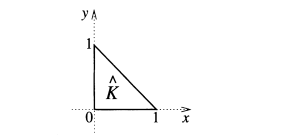
\includegraphics[width=0.33\textwidth]{referenzzelle.png} \\
	Abbildung aus \cite{knabner2013numerik} Seite 51
\end{figure}

\begin{Bemerkung}
	$\forall i,j\in\{1,2,3\}: \int_{F_j} \hat{\psi}_i \cdot \hat{n} \da = \delta_{i,j} \text{ und } \hat{\psi}_i \in \mathbb{P}_1(\hat{K}, \R^2).$
\end{Bemerkung}

Weiter setzen wir noch 
\begin{align*}
\text{ die Menge der Seiten }&& \hat{\mathcal{F}} &\coloneqq \left\{ \hat{F}_0, \hat{F}_1, \hat{F}_2 \right\} \\
\text{und den Seitenansatzraum }&&  \hat{W} &\coloneqq \spann \left\{ \psi_0,\psi_1, \psi_2 \right\}.
\end{align*}
\textbf{Transformation von $ \hat{K} $ zu $ K $:} Für ein beliebiges $ K \in \mathcal{K} $ wollen wir jetzt eine Seitenbasis $ \{ \psi_1^K, \psi_2^K, \psi_3^K \} $ berechnen (Wie bisher gegeben durch $ \forall i\in\{1,2,3\}: \psi_i^K\in\mathbb{P}_1(K,\R^2) \text{ und } \int_{F_j^K} \psi_i^K \cdot n^K \da = \delta_{i,j} $, wobei $ n^K $ äußere Normale von  $ K $ und $ F_j^K  $ beliebige Seite von $ K $). Dazu betrachten wir die affine Transformationsabbildung $ \varphi_K $ von $ \hat{K} $ zu $ K $:
\begin{align*}
\varphi_K: \hat{K} \to K, \varphi_K(\xi) = z_{0,K} + B_K \xi \text{ mit passenden } B_K\in\R^{2 \times 2} \text{ und } \\
J_K \coloneqq \det(B_K) > 0.
\end{align*}

\begin{figure}[H]
	\centering
	\captionabove{Affine lineare Transformation von $\hat{K}$ nach $ K $}
	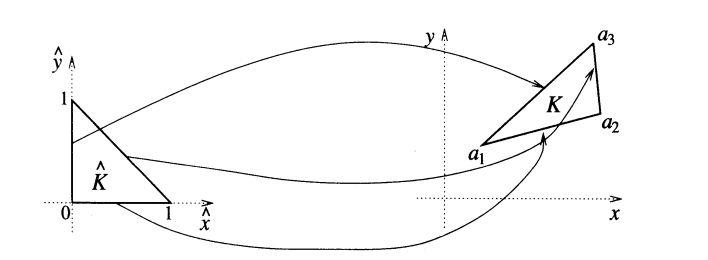
\includegraphics[width=0.55\textwidth]{affinlinearetransf.png} \\
	Abbildung aus \cite{knabner2013numerik} Seite 53
\end{figure} 

\begin{Lemma}
	Es gilt: $\tilde{n}^K = \frac{1}{\abs{B_K^{-T} \hat{n}}} B_K^{-T} \hat{n} $ ist Normale zu $ \partial K $.
\end{Lemma}

Die Seitenbasis auf $ K $ ist dann gegeben durch 
\[ \psi_i^K = J_K^{-1}B_K \hat{\psi}_i \circ \varphi_K \ (i\in \{1,2,3\}) \]

Die globale Seitenbasis $\{\psi_j\}_{j = 1}^{\abs{\mathcal{F}}}$ auf $ \mathbb{D}  $ erhalten wir dann mithilfe einer weiteren Abbildung $l$ die zwischen der Seitennummerierung in einer Zelle $ K $ und der globalen Seitennummerierung vermittelt. Es ist dabei
\[ l:\mathcal{K}\times \{1,2,3\} \to \{1, \dots , \abs{\mathcal{F}} \}, (K,i) \mapsto l(K,i). \]
Wir setzen nun also $ \psi_j (j \in \{1,\dots , \abs{\mathcal{F}}\})$ durch
\[ \psi_j(x) = 
\begin{cases}
\psi_i^K(x) , &\text{falls } j = l(K,i)\\
0,			  &\text{sonst}.
\end{cases} \]
\begin{Bemerkung}
	Für alle Zellen $ K \in \mathcal{K} $ von denen $ F_j $ eine anliegende Seite ($ \overline{K} \cap F_j \ne \emptyset $) und $ F_j $ lokal mit $ i \in \{1,2,3\} $ nummeriert ist, gilt:
	\[ \psi_j|_K = \psi_i^K. \]
\end{Bemerkung}

\subsubsection{Hybridisierung}

Wir betrachten die Räume
\[W_K \coloneqq \left\{ \psi_K:K \to \R^2: \psi_K = J_K^{-1}  B_K \hat{\psi} \circ \varphi_K^{-1}, \hat{\psi} \in \hat{W} \right\} \]
\[ W_\mathcal{K} \coloneqq \prod_{K \in \mathcal{K}} W_K, \qquad M_h \coloneqq \prod_{F \in \mathcal{F}} \mathbb{P}_0(F) \]
\[ M_h(u_D) \coloneqq \left\{ \mu_h \in M_h:\forall  F \subset \Gamma_D \int_F \mu_h \da = \int_F u_D \da  \right\}\]

\begin{Bemerkung}~
	
	$ \psi_h \in W_h \iff \big[ \psi_h \in W_{\mathcal{K}} \text{ und }  (\psi_{K_1} - \psi_{K_2}) \cdot n^F = 0 \ (F= \partial K_1 \cap \partial K_2 \in \mathcal{F}^{\circ})\big] $
\end{Bemerkung}


Und untersuchen folgendes Problem:
\begin{align*}
\text{Bestimmme } (q_h,u_h, \lambda_h) \in W_\mathcal{K} \times Q_h \times M_h(u_D) \text{ mit}\\
\begin{dcases}
(1) \int_K \kappa^{-1} q_h \psi_K \dx - \int_K u_h \dive(\psi_K) \dx = - \int_{\partial K} \lambda_h \psi_K \cdot n^K \da \\
(2) \int_K \dive(q_h) \phi_K \dx = 0\\
(3) \sum_{K\in \mathcal{K}} \int_{\partial K} q_h \cdot n \mu_h \da = - \int_{\Gamma_N} g_N \mu_h \da
\end{dcases}\\
\text{für alle } K \in \mathcal{K}, \psi_K \in W_K, \phi_K \in Q_h  \text{ und } \mu_h \in M_h(0)
\end{align*}

Dieses Problem ist äquivalent zu dem diskreten gemischten FE-Problem, welches wir zuvor betrachtet haben:
\begin{align*}
\text{Bestimme } (q_h,u_h) \in W_h(-g_N) \times Q_h \text{ mit}\\
\begin{cases}
\int_{\Omega} \kappa ^{-1} q_h \cdot \psi_h \dx \mkern-15mu &- \int_{\Omega} u_h \dive(\psi_h) \dx = - \int_{\Gamma_D} u_D \psi_h \cdot n \da\\
&- \int_{\Omega} \dive(q_h) \phi_h \dx = 0
\end{cases} \\
\text{für alle } (\psi_h, \phi_h) \in W_h(0) \times Q_h
\end{align*}

Für ein festes $ K \in \mathcal{K} $ ergibt sich mit der Wahl einer Basis von $ W_K $, $ Q_h $ und $ M_h $ 
%\begin{align*}
%	&W_K = \spann\{\psi_F \mid F \in \mathcal{F}_K \}  &&(\psi_F \cdot n^F)_{|F'} = \begin{cases}
%		1 &F = F'\\
%		0 &\text{sonst}
%	\end{cases}\\
%	&Q_h = \spann\{\eta_K \mid K \in \mathcal{K}  \}  &&{\eta_K}_{|K'} = \begin{cases}
%	1 &, K = K'\\
%	0 &,\text{sonst}
%	\end{cases}\\
%	&M_h = \spann \{ \nu_F \mid F \in \mathcal{F}_K \}  &&{\nu_F}_{|F'} = \begin{cases}
%		1 &, F = F'\\
%		0 &, \text{sonst}
%	\end{cases}  
%\end{align*}

eine Formulierung als LGS mit Nebenbedingung, wobei $ \ubar{q}_K \coloneqq \ubar{R}_K \ubar{q}, \ \ubar{u}_K \coloneqq \ubar{R}_K \ubar{u} $
\begin{align*}
\text{Bestimme } \ubar{q}, \ubar{u} \text{ und } \ubar{\lambda} \text{ mit}\\
\begin{dcases}
(1) \begin{pmatrix}
\ubar{A}_K & \ubar{B}_K \\
\ubar{B}_K^T & 0
\end{pmatrix}
\begin{pmatrix}
\ubar{q}_K\\
\ubar{u}_K
\end{pmatrix}
\mkern-16mu&= \begin{pmatrix}
- \ubar{C}_K \, \ubar{R}_K \ubar{\lambda} \\
0
\end{pmatrix}\\
(2) \sum_{K \in \mathcal{K}}  (\ubar{R}_K \ubar{\mu})^T \ubar{C}_K \ubar{q}_K \mkern-16mu&= \ubar{\mu}^T \ubar{b}		
\end{dcases}\\
\text{für alle } \ubar{\mu} \text{ mit } \ubar{\mu}[F] = 0 \text{ für } F \in \Gamma_D \cap \mathcal{F}
\end{align*}

\begin{align*}
\left(
\begin{array}{c}
1\\ 1 \\ \vdots \\ 1 \\ 1\\ \ubar{\mu}
\end{array}
\right)^T
\underbrace{\left(
	\begin{array}{ccccc|c}
	\ubar{A}_{K_1} & \ubar{B}_{K_1}&&&& \ubar{C}_{K_1} \ubar{R}_{K_1}\\
	\ubar{B}_{K_1} & 0 &&&& 0\\
	&& \ubar{A}_{K_2} & \ubar{B}_{K_2} && \ubar{C}_{K_2} \ubar{R}_{K_2}\\
	&  & \ubar{B}_{K_2} & 0 && 0\\
	&  &  &  &\ddots &\\
	\hline
	\ubar{R}_{K_1}^T \ubar{C}_{K_1}^T& 0 & \ubar{R}_{K_2}^T \ubar{C}_{K_2}^T& 0& &0 \\
	\end{array}
	\right)}_{\eqqcolon \left( \begin{array}{c|c}
	\ubar{D} & \ubar{E}\\
	\hline
	\ubar{E}^T & 0
	\end{array} \right)}
\underbrace{\left(
	\begin{array}{c}
	\ubar{q}_{K_1}\\ \ubar{u}_{K_1} \\ \ubar{q}_{K_2}\\ \ubar{u}_{K_2} \\ \vdots \\ \ubar{\lambda}
	\end{array}
	\right)}_{\eqqcolon \left( \begin{array}{c}
	\left(
	\begin{array}{c}
	\ubar{q}_{K_i}\\ \ubar{u}_{K_i}
	\end{array}
	\right)_{K_i \in \mathcal{K}} \\ \ubar{\lambda} 
	\end{array}\right)} = 
\left(
\begin{array}{c}
0\\ 0 \\ \vdots \\ 0 \\ 0\\ \ubar{\mu}^T \ubar{b}
\end{array}
\right)
\end{align*}
Mit dem Schurkomplement $ \ubar{S} \coloneqq \ubar{E}^T \ubar{D}^{-1} \ubar{E} $ folgt
\[ \ubar{\mu}^T \ubar{S} \, \ubar{\lambda} = \ubar{\mu}^T \ubar{b} 	\text{ für alle } \ubar{\mu} \text{ mit } \ubar{\mu}[F] = 0 \text{ für } F \in \Gamma_D \cap \mathcal{F} \]

Sobald wir $ \ubar{\lambda}_k \coloneqq \ubar{R}_K \ubar{\lambda}$ bestimmt haben, können wir auch das obere LGS (1) lösen um $ \ubar{q}_K $ und $ \ubar{u}_K $ zu erhalten.
% Um $ \ubar{\lambda}_k $ zu erhalten lösen wir das globales System:
%\begin{align*}
%	\underline{S} \, \underline{\lambda} = \underline{b}
%\end{align*}
%und bekommen somit $ \ubar{\lambda}_k $ über die Restriktionen
%\[ \ubar{\lambda} = \sum_{K \in \mathcal{K}} \ubar{R}_K \ubar{\lambda}_K .\]

\subsection{Jupyter-Notebook}
Zuletzt wollen wir noch das Jupyter-Notebook angeben, mit welchem es möglich ist die gezeigten Ergebnisse zu reproduzieren. Es findet sich in \cite{branchMLMCTP} im Unterordner $'notebooks'$ unter dem Namen $'mlmc\_transport.ipynb'$. Ebenfalls ist in \cite{branchMLMCTP} eine Installationsanleitung zu finden. 
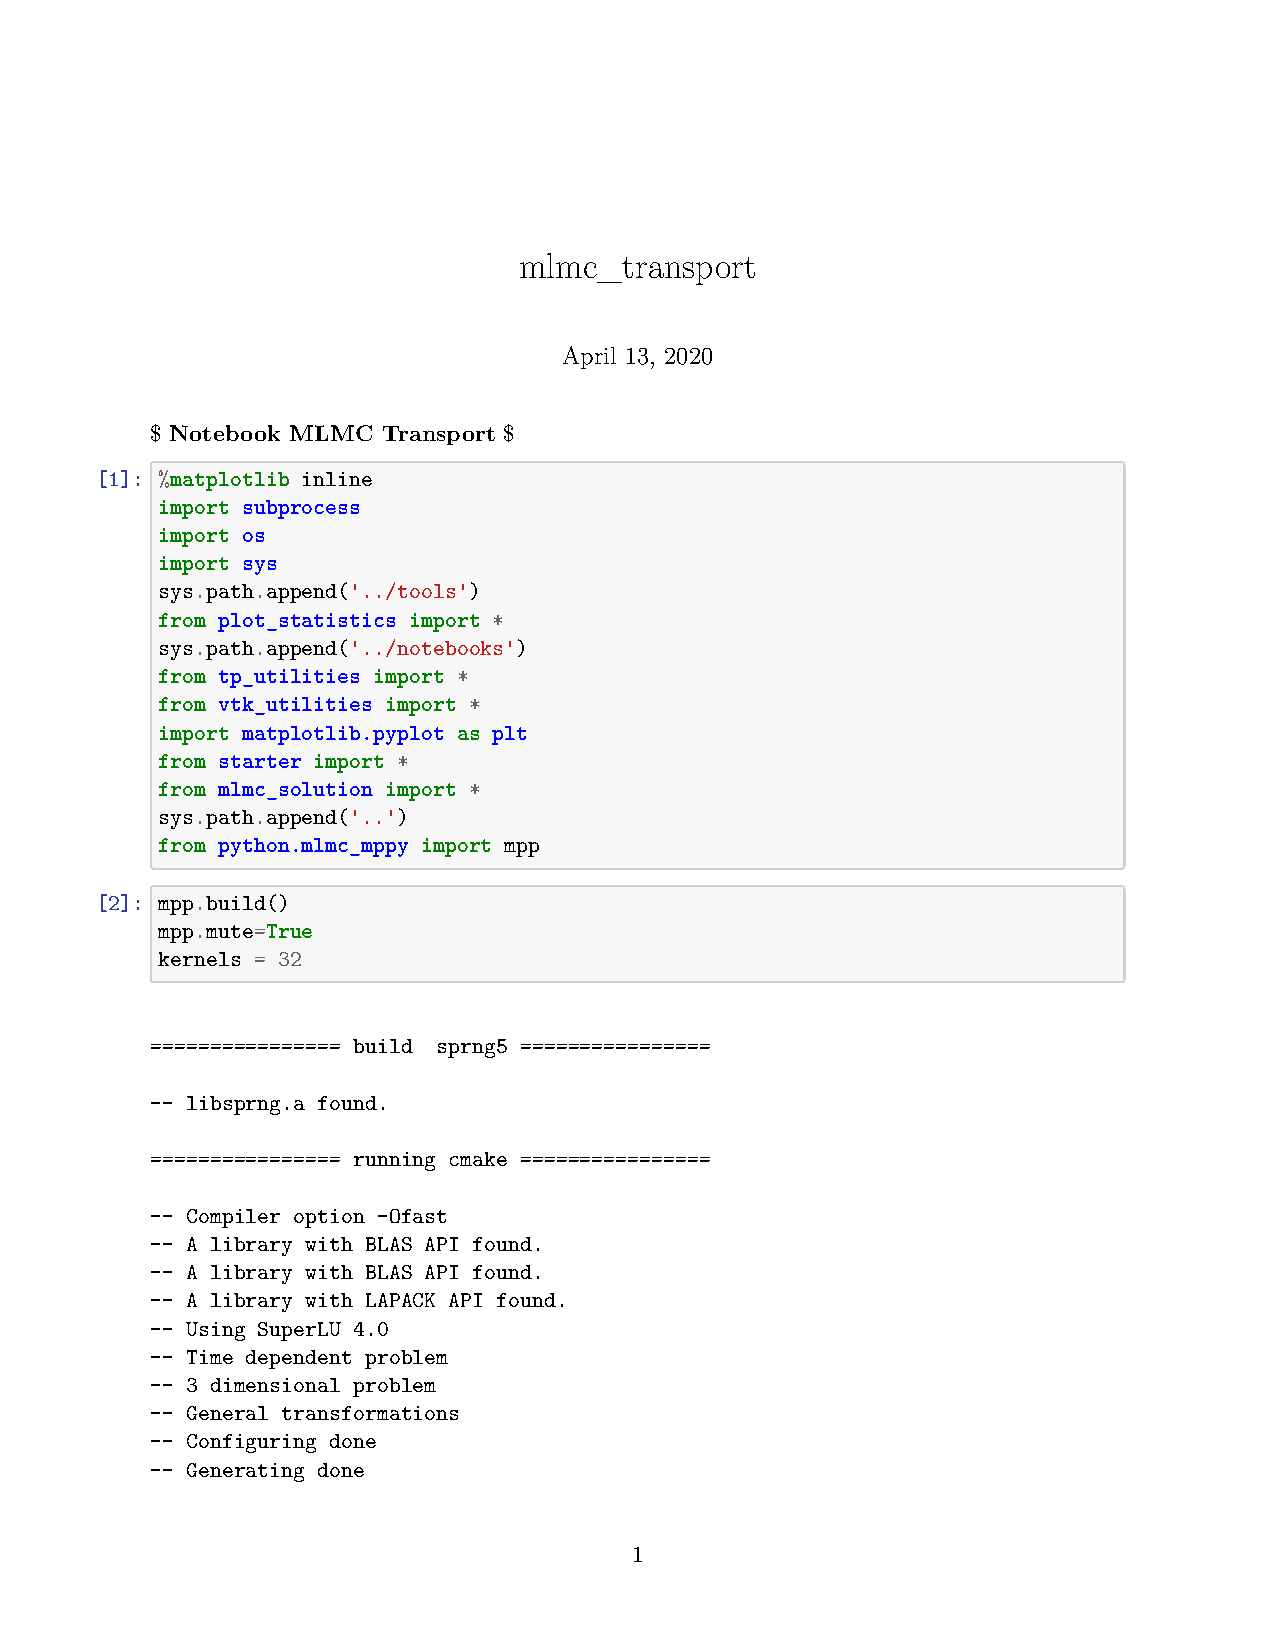
\includepdf[pages=-]{mlmc_transport.pdf}

  % Literaturverzeichnis (beginnt auf einer ungeraden Seite)
  \newpage

%\begin{thebibliography}{Lam00}
 %Bibiographie
  \bibliographystyle{abbrv}
  \bibliography{References}
%\end{thebibliography}
 
      
  % ggf. hier Tabelle mit Symbolen 
  % (kann auch auf das Inhaltsverzeichnis folgen)

\newpage
  
 \thispagestyle{empty}


\vspace*{8cm}


\section*{Erkl\"arung}

Ich  versichere  wahrheitsgem\"a\ss,  die  Arbeit selbstst\"andig verfasst,  alle  benutzten  Hilfsmittel  vollst\"andig  und  genau  angegeben  und  alles kenntlich  gemacht  zu  haben,  was  aus  Arbeiten  anderer  unver\"andert  oder  mit  Ab\"anderungen entnommen  wurde,  sowie die Satzung  des  KIT  zur  Sicherung guter wissenschaftlicher Praxis in der jeweils g\"ultigen Fassung beachtet zu haben.
\\[2ex] 

\noindent
Karlsruhe, den 19.04.20\\
\includegraphics*[width=0.31\textwidth]{unterschrift.png}
% Unterschrift (handgeschrieben)



\end{document}

